
%--------Dokumentenart-----------------------------------------------------------------------

\documentclass[DIV12,BCOR10mm,headsepline,twoside,a4paper,11pt]{scrreprt}

%--------Einbinden der Packages--------------------------------------------------------------

\usepackage{ngerman}
%\usepackage[utf8]{inputenc}
\usepackage[ansinew]{inputenc}
\usepackage[T1]{fontenc}
\usepackage{iflstyle}
\usepackage{german}
\usepackage{bibgerm} %chicago
\usepackage{url}
\usepackage{paralist}
\usepackage{amsmath}
\usepackage{xcolor}
\usepackage{enumitem}

% Jelsch
\usepackage{listings}

\usepackage{color}
\definecolor{SQLBlue}{RGB}{0,102,153}
\definecolor{SQLGreen}{RGB}{184,217,119}
\definecolor{SQLOrange}{RGB}{250,151,73}
\definecolor{SQLGray}{RGB}{237,237,237}

\definecolor{Set1-6-1}{RGB}{90,155,213}
\definecolor{Set1-6-2}{RGB}{165,165,165}
\definecolor{Set1-6-3}{RGB}{67,114,196}
\definecolor{Set1-6-4}{RGB}{196,114,67}

\lstdefinelanguage{RDF}
{
  basicstyle={\small\upshape},
  breaklines=true,
  frame=single,
  tabsize=2,
  xleftmargin={1cm},
  numbers=left,
  stepnumber=1,
  firstnumber=1,
  numberfirstline=true,
  language={XML},
  captionpos=b,
  columns=fullflexible,
  showstringspaces=false,
  keywordstyle=\bfseries\color{SQLBlue},
  commentstyle=\color{gray}\upshape,
  identifierstyle=\color{SQLGreen},
  stringstyle=\color{blue},
  otherkeywords={COLUMNS},
  deletekeywords={YEAR}
}

\lstdefinelanguage{Turtle}
{
  morestring=[b]",
  morestring=[s]{>}{<},
  morecomment=[s]{<?}{?>},
  stringstyle=\color{black},
  identifierstyle=\color{SQLBlue},
  keywordstyle=\color{cyan},
  morekeywords={xmlns,version,type}
}

\lstdefinelanguage{MDX}
{
  basicstyle={\small\upshape},
  breaklines=true,
  frame=single,
  tabsize=2,
  xleftmargin={1cm},
  numbers=left,
  stepnumber=1,
  firstnumber=1,
  numberfirstline=true,
  language={SQL},
  captionpos=b,
  columns=fullflexible,
  showstringspaces=false,
  keywordstyle=\bfseries\color{SQLBlue},
  commentstyle=\color{gray}\upshape,
  identifierstyle=\color{black},
  stringstyle=\color{blue},
  otherkeywords={COLUMNS},
  deletekeywords={YEAR}
}

\colorlet{punct}{red!60!black}
\definecolor{background}{HTML}{EEEEEE}
\definecolor{delim}{RGB}{20,105,176}
\colorlet{numb}{magenta!60!black}

\lstdefinelanguage{json}{
  literate=
   *{0}{{{\color{numb}0}}}{1}
    {1}{{{\color{numb}1}}}{1}
    {2}{{{\color{numb}2}}}{1}
    {3}{{{\color{numb}3}}}{1}
    {4}{{{\color{numb}4}}}{1}
    {5}{{{\color{numb}5}}}{1}
    {6}{{{\color{numb}6}}}{1}
    {7}{{{\color{numb}7}}}{1}
    {8}{{{\color{numb}8}}}{1}
    {9}{{{\color{numb}9}}}{1}
    {:}{{{\color{punct}{:}}}}{1}
    {,}{{{\color{punct}{,}}}}{1}
    {\{}{{{\color{delim}{\{}}}}{1}
    {\}}{{{\color{delim}{\}}}}}{1}
    {[}{{{\color{delim}{[}}}}{1}
    {]}{{{\color{delim}{]}}}}{1},
}


\lstset{
    basicstyle={\small\upshape},
    breaklines=true,
    frame=single,
    tabsize=2,
    xleftmargin={1cm},
    numbers=left,
    stepnumber=1,
    firstnumber=1,
    numberfirstline=true,
    language={SQL},
    captionpos=b,
    columns=fullflexible,
    showstringspaces=false,
    keywordstyle=\bfseries\color{SQLBlue},
    commentstyle=\color{gray}\upshape,
    identifierstyle=\color{black},
    stringstyle=\color{blue},
    otherkeywords={ROW,FORMAT,SERDE,WITH,SERDEPROPERTIES,STORED,LOCATION,STRING,PARTITION,PARTITIONED,DOUBLE,INT}
}

%---------Kompilieren mit Latex oder PdfLatex-------------------------------------------------
\usepackage{ifpdf}
\ifpdf
  \usepackage[pdftex]{graphicx}
  \usepackage[pdftex, colorlinks=true, linkcolor={black}, urlcolor={black}, citecolor={black}]{hyperref}
  \DeclareGraphicsExtensions{.jpg,.pdf,.tif,.png}
  \graphicspath{{images/}}
  \pdfcompresslevel=0
  \pdfcatalog{/ViewerPreferences <</FitWindow true>>}
  \pdfinfo{
      /Title (Diplomarbeit)
      /Author (S�bastien Jelsch)
      /Subject (Optimierung von Analytischen Abfragen �ber Statistical Linked Data durch Horizontale Skalierung)
      /CreationDate (07.01.2016)
  }
\fi
%-----------------------------------------------------------------------------------------

\usepackage{tikz}
\usetikzlibrary{shapes.geometric}
\usetikzlibrary{arrows}
\usepackage{rotating}
\usepackage{multirow}
\usepackage{pgfplots, pgfplotstable}
\usepackage{acronym} % f�r Abk�rzungen %[printonlyused]

\pagestyle{headings}

\begin{document}

\ifltitle{Diplomarbeit}
         {}
         {Optimierung von Analytischen Abfragen �ber Statistical Linked Data durch Horizontale Skalierung}
         {S�bastien Jelsch}
         {Dipl.-Inform.~Benedikt K�mpgen}
         {Karlsruhe, Januar 2016}
         {}
\iflrecht{S�bastien Jelsch}
         {Karlsruhe, 07.01.2016}

%Verzeichnisse
  \pagestyle{headings}
  \pagenumbering{roman}
  \setcounter{page}{1}
  \blankpage

\chapter*{Kurzzusammenfassung}
\addcontentsline{toc}{chapter}{Kurzzusammenfassung}

In den letzten Jahren ist die Menge der verf�gbaren Linked Data im World Wide Web stetig gestiegen. Immer mehr Provider ver�ffentlichen ihre statistischen Datens�tze nach dem Linked-Data-Prinzip, um diese Daten mit weiteren Informationen aus unterschiedlichen Quellen anreichern zu k�nnen. Durch die Verlinkung beliebiger Zusatzinformationen sollen die Daten n�her bestimmt und neue Erkenntnisse erlangt werden.

Bevor Analysten jedoch in der Lage sind, solche statistischen Daten vergleichen zu k�nnen, verbringen sie unverh�ltnism��ig viel Zeit mit der Identifizierung, Erfassung und Aufbereitung der relevanten Daten. Zus�tzlich f�hrt die zunehmende Gr��e an verf�gbaren RDF-Datens�tzen dazu, dass diese nicht mehr effizient auf einem einzelnen Rechner analysiert werden k�nnen. Aus diesem Grund sind f�r Analysen gro�er Datenmengen Technologien aus dem Big-Data-Umfeld notwendig, die diese Beschr�nkungen mittels Parallelisierung �ber viele Rechner hinweg �berwinden. In der Folge ist f�r die Analyse einer beliebig gro�en RDF-Datenmenge ein L�sungsansatz erforderlich, der diese Datens�tze generisch und automatisiert in ein horizontal skalierbares Open Source OLAP-System integriert, die Daten in geeigneter Form aufbereitet und dem Nutzer pr�sentiert.

In dieser Arbeit wird ein horizontal skalierbarer Extract-, Transform- und Load-Prozess (ETL-Prozess) konzipiert, umgesetzt und im Hinblick auf die Ausf�hrungszeit f�r die Integration der RDF-Daten in das OLAP-System Apache Kylin evaluiert. Des Weiteren werden die Antwortzeiten analytischer MDX- und SQL-Abfragen untersucht. Die Ergebnisse zeigen, dass der ETL-Prozess erst ab einer gr��eren Datenmenge einen Vorteil gegen�ber Import-Vorg�ngen in nicht-horizontal skalierenden Systemen bietet. Jedoch werden analytische Abfragen in diesem System aufgrund der horizontalen Skalierung in sehr kurzer Zeit beantwortet.

\textbf{Schl�sselw�rter:} Linked Data, Data Cube, Parallelisierung, MapReduce


  \cleardoublepage
  \phantomsection
  \addcontentsline{toc}{chapter}{Inhaltsverzeichnis}
  \tableofcontents

  \cleardoublepage
  \phantomsection
  \addcontentsline{toc}{chapter}{Abbildungsverzeichnis}
  \listoffigures

  \cleardoublepage
  \phantomsection
  \addcontentsline{toc}{chapter}{Tabellenverzeichnis}
  \listoftables

  \cleardoublepage
  \phantomsection
  \addcontentsline{toc}{chapter}{Textboxenverzeichnis}
  \lstlistoflistings

  \cleardoublepage
  \phantomsection
  \addcontentsline{toc}{chapter}{Abk�rzungsverzeichnis}
  %% abkuerzungen.tex
\markboth{Abk�rzungsverzeichnis}{Abk�rzungsverzeichnis}

\chapter*{Abk�rzungsverzeichnis}
\label{ch:Abkuerzungen}
%% ==============================

\begin{acronym}
\acro{API}{Application Programming Interface}
\acro{AWS}{Amazon Web Services}
\acro{BI}{Business Intelligence}
\acro{BIBM}{Business Intelligence Benchmark}
\acro{CDH}{Cloudera Distribution Including Apache Hadoop}
\acro{DSD}{Data Structure Definiton}
\acro{EC2}{Elastic Compute Cloud}
\acro{ETL-Prozess}{Extract-, Transform- und Load-Prozess}
\acro{FOAF}{Friend of a Friend}
\acro{HDFS}{Hadoop Distributed File System}
\acro{HiveQL}{Hive Query Language}
\acro{HTTP}{Hypertext Transfer Protocol}
\acro{JDBC}{Java Database Connection}
\acro{MDM}{Multidimensionales Datenmodell}
\acro{MDX}{Multidimensional Expression}
\acro{MOLAP}{Multidimensionales OLAP}
\acro{NoSQL}{Not only SQL}
\acro{OLAP}{On-Line Analytical Processing}
\acro{QB}{RDF Data Cube Vocabulary}
\acro{RDF}{Resource Description Framework}
\acro{RDFS}{RDF Schema}
\acro{ROLAP}{Relationales OLAP}
\acro{SPARQL}{SPARQL Protocol And RDF Query Language}
\acro{SQL}{Structured Query Language}
\acro{SSB}{Star Schema Benchmark}
\acro{URI}{Uniform Resource Identifier}
\acro{W3C}{World Wide Web Consortium}
\acro{XML}{Extensible Markup Language}
\end{acronym}

% \acro{Name}{Darstellung der Abk�rzung}{Langform der Abk�rzung}
% Folgendes benutzen, wenn der Plural einer Abk. ben�igt wird
% \newacroplural{Name}{Darstellung der Abk�rzung}{Langform der Abk�rzung}
% \newacroplural{Abk}[Abk-en]{Abk�rzungen}


  \cleardoublepage

%Kapitel
  \pagenumbering{arabic}
  \chapter{Einleitung}
\label{Einleitung}

Das heutige World Wide Web (kurz: Web) besitzt aufgrund seiner rasanten Entwicklung eine f�r Menschen un�berschaubare, stetig wachsende Menge an Informationen. Neben den Vorteilen der universellen Verf�gbarkeit, der st�ndigen Aktualit�t und der einfachen Bereitstellung von Daten �berwiegt jedoch ein wesentlicher Nachteil: die Ausrichtung der Informationen orientiert sich an einem menschlichen Betrachter. Im Gegensatz zu einer Maschine kann ein menschlicher Benutzer die Bedeutung von Informationen auf einer Webseite erfassen, zueinander in Beziehung setzen und in eine andere Darstellungsform transformieren, um neues Wissen zu generieren. Die Datenf�lle und dezentrale Organisation des Webs f�hren dazu, dass eine Suche nach gew�nschten Informationen erschwert wird. Erstrebenswert ist daher eine inhaltliche und semantische Suche.

Hierzu pr�gte Tim Berners-Lee 2001 das Konzept Semantic Web. Die Grundidee des Konzepts besteht darin, das herk�mmliche Web durch Standards zu erweitern. Im Vordergrund steht dabei die Verwertung der Informationen von Maschinen und der einfache Austausch zwischen diesen. Dazu sind grundlegende Anforderungen notwendig, die neben einer klaren Definition des Standards auch eine flexible Anwendung und m�gliche Erweiterungen erlauben sollen.

Aus diesem Grund wurde das Resource Description Framework (RDF) entwickelt. RDF ist eine Modellierungssprache zur Beschreibung strukturierter Informationen und ein Standard des World Wide Web Consortium. Mit dem RDF-Standard soll es Anwendungen erm�glicht werden, Daten �ber das Web auszutauschen, ohne ihre eigentliche Bedeutung zu verlieren und sie mit zus�tzlichen Informationen aus anderen Datenquellen anzureichern. Im Gegensatz zum herk�mmlichen Web geht es hierbei nicht nur um eine korrekte Darstellung von Daten oder Dokumenten, sondern vielmehr um die Verkn�pfung von Daten aus unterschiedlichen Quellen f�r die Weiterverarbeitung der Informationen.

\newpage

\section{Motivation}
\label{Motivation}

In den letzten Jahren ist das Interesse gestiegen, statistische Daten nach dem Linked-Data-Prinzip zu ver�ffentlichen und die M�glichkeit zu bieten, Daten mit anderen Informationen aus unterschiedlichen Quellen zu kombinieren. Ein Vorteil besteht darin, beliebige Zusatzinformationen zu den statistischen Daten zu verlinken, um die Bedeutung der Daten n�her zu bestimmen und neue Erkenntnisse zu erlangen. Beispielsweise k�nnen Provenance-Informationen (z.\,B. Woher stammen die Daten? Welche Qualit�t besitzen sie?) oder weitergehende Informationen (z.\,B. Welche Anzahl an Mitarbeitern besitzt die Firma, von denen die Daten handeln?) hinzugef�gt werden. Ferner k�nnen auch interne Daten (z.\,B. aus dem Intranet) einer Firma mit den statistischen Daten verlinkt und zur Analyse verwendet werden.

Bevor Analysten jedoch in der Lage sind, Unternehmensleistungen vergleichen zu k�nnen, verbringen sie unverh�ltnism��ig viel Zeit mit der Identifizierung, Erfassung und Aufbereitung der relevanten Daten. Der Aufwand steigt mit der Anzahl heterogener Datenquellen. Damit verbunden sind unterschiedliche Formate oder Bezeichnungen f�r identische Objekte. Diese Prozesse m�ssen optimiert und m�glichst automatisiert werden. Zus�tzlich f�hrt die zunehmende Gr��e an verf�gbaren RDF-Datens�tzen\footnote{ s. Datens�tze, die nach dem Linked-Data-Prinzip ver�ffentlicht werden: \url{http://lod-cloud.net/}.} dazu, dass diese nicht mehr effizient auf einem einzelnen Rechner verarbeitet und analysiert werden k�nnen. Daher sind neue Konzepte zur Auswertung statistischer Datens�tze notwendig. Ferner ist ein L�sungsansatz erforderlich, der eine beliebig gro�e RDF-Datenmenge generisch und automatisiert integriert, diese in geeigneter Form aufbereitet und dem Nutzer pr�sentiert.

\section{Zielsetzung}
\label{Zielsetzung}

F�r entscheidungsunterst�tzende Analysen numerischer Datens�tze bietet das Konzept OLAP (\textbf{O}n-\textbf{L}ine \textbf{A}nalytical \textbf{P}rocessing) eine multidimensionale Betrachtung des Datenbestands. In einer vorangegangenen Arbeit von K�mpgen und Harth \cite{kampgen2011transforming} wurde hierf�r ein Extract-, Transform- und Load-Prozess (ETL-Prozess) vorgestellt, der statistische Linked Data aus unterschiedlichen RDF Stores, unter Anwendung der Abfragesprache \mbox{SPARQL} und dem RDF Data Cube Vocabulary (QB), in ein multidimensionales Datenmodell transformiert. Die Daten wurden f�r die Analysen in einem relationalen Data Warehouse gespeichert. Auf diese Weise konnte mit der OLAP-to-SQL-Engine Mondrian die Vorteile der multidimensionalen Abfragem�glichkeit und erweiterten Selektierbarkeit von OLAP-Anfragen mit MDX (engl. f�r \textbf{M}ulti\textbf{D}imensional E\textbf{X}pression) genutzt werden. Ziel des ETL-Prozesses war es, entscheidungsunterst�tzende Analysen auf RDF-Datens�tzen durchzuf�hren. Dieser Ansatz beinhaltet jedoch vier wesentliche Probleme:

\begin{compactenum}[(V1)]
\item Die Dauer des ETL-Prozesses bei gro{\ss}en Datens�tzen mit vielen Zusatzinformationen ist nicht zufriedenstellend, da innerhalb der RDF-Daten die n�tigen Informationen f�r das multidimensionale Datenmodell (Metadaten und Daten) herausgezogen werden m�ssen.
\item Bei einer Aktualisierung des Datenbestands muss der ETL-Prozess neu durchgef�hrt werden.
\item Bei der Hinzunahme neuer Daten muss der ETL-Prozess ebenfalls neu durchgef�hrt werden.
\item Zusatzinformationen in den Datens�tzen werden bei der Erstellung des multidimensionalen Datenmodells gefiltert und k�nnen in den analytischen Abfragen nicht ber�cksichtigt oder als Zusatzinformation abgefragt werden.
\end{compactenum}

Sowohl relationale Datenbanken, RDF Stores als auch OLAP Engines skalieren in der Regel nicht horizontal und besitzen daher eine nat�rliche Grenze bzgl. ihrer Datenspeicher- und Datenverarbeitungskapazit�t. Aus diesem Grund sind f�r Analysen gro{\ss}er Datenmengen Technologien aus dem Big-Data-Umfeld notwendig, die diese Beschr�nkungen mittels Parallelisierung �ber viele Rechner hinweg �berwinden. Mit Apache Hadoop sind derartige Technologien in einem Open Source Software Stack verf�gbar. Bislang wurde nicht erforscht, ob eine enorm gro�e RDF-Datenmenge in einem automatisierten ETL-Prozess durch eine Umsetzung der Architektur von K�mpgen und Harth mit Komponenten aus dem Hadoop-�kosystem f�r OLAP-Analysen bereitgestellt werden kann.

Der hier pr�sentierte L�sungsansatz �berf�hrt K�mpgen und Harths Konzept in eine horizontal skalierende Architektur auf der Basis von Apache Hadoop. Die nicht-skalierbaren Komponenten, wie die RDF-Datenbank, die Abfragesprache \mbox{SPARQL} und die relationale Datenbank, werden dabei durch Technologien und Frameworks aus dem Hadoop-�kosystem ersetzt.

Eine weitere Zielsetzung dieser Arbeit liegt in der generischen und automatisierten Umsetzung des ETL-Prozesses unter Verwendung der Metainformationen des QB-Vokabulars. Ferner soll der ETL-Prozess auf seine Ausf�hrungszeit im Hinblick auf die Anzahl der verwendeten Rechner im Vergleich zur relationalen Datenbank MySQL und dem RDF Store Open Virtuoso evaluiert werden.

\section{Verwandte Arbeiten}
\label{Verwandte-Arbeiten}

In einer vorherigen Arbeit \cite{NoSize} wurden die statistischen Daten in einem RDF Store geladen, um analytische Abfragen mittels der graphenbasierten Sprache SPARQL auszuf�hren. Es zeigte sich, dass die Ausf�hrung der analytischen Abfragen weniger effizient durchgef�hrt wurden, als vergleichsweise eine relationale Datenbank mit �quivalenten Daten im Sternschema. Eine weitere Arbeit~\cite{NoSQL} besch�ftigte sich mit der Optimierung eines RDF Stores durch horizontale Skalierung. Da NoSQL-Systeme f�r komplexe OLAP-Operationen weniger geeignet sind, war die Ausf�hrung der analytischen Abfragen nicht effizient genug. In der Arbeit von Abell� et al.~\cite{Abello} wurden analytische Abfragen auf MapReduce-basierten Systemen evaluiert. Dabei wurden die Vorteile von Big-Data-Technologien bei der Generierung eines OLAP Cubes f�r analytische Abfragen �berpr�ft, jedoch ohne eine horizontale skalierbare OLAP Engine f�r die Analysen zu verwenden. Zusammenfassend kann festgestellt werden, dass eine Analyse einer beliebig gro�en Menge an RDF-Daten eine Herausforderung darstellt.

\section{Gliederung}
\label{Gliederung}

Die vorliegende Arbeit ist in sechs Kapitel unterteilt. Das erste Kapitel gibt dem interessierten Leser eine kurze Einf�hrung und einen Gesamt�berblick �ber die geplanten Ziele. Das zweite Kapitel enth�lt eine ausf�hrliche Beschreibung der Grundlagen und der verwendeten Begriffe, wobei der Fokus auf traditionellen Konzepten f�r Analysen statistischer Datens�tze, der Idee hinter dem Semantic Web und auf die in dieser Arbeit verwendeten Big-Data-Technologien im Verbund mit Apache Hadoop und sein �kosystem liegt. Der dritte Abschnitt beschreibt das in dieser Arbeit entworfene Konzept und die Gesamtarchitektur. Zudem werden die verwendeten Komponenten aus dem Apache Hadoop-�kosystem sowie ihr Zusammenspiel in diesem Abschnitt einer n�heren Betrachtung unterzogen. Das vierte Kapitel beschreibt die technische Umsetzung des ETL-Prozesses. Auf den Evaluationsaufbau und die erhaltenen Ergebnisse wird im f�nften Kapitel eingegangen. Anschlie�end werden im letzten Kapitel das Fazit der Arbeit und m�gliche Erweiterungen besprochen.

  \chapter{Grundlagen}
\label{cha:Grundlagen}

In diesem Kapitel werden die in der Abschlussarbeit verwendeten Begriffe und Notationen erl�utert. Der erste Abschnitt beschreibt die wesentlichen Anforderungen f�r die Analyse statistischer Datens�tze sowie die daraus entstandenen Konzepte und Prozesse. Im Vordergrund steht dabei die Definition des Begriffs \textit{Business Intelligence}, die grundlegenden Aufgaben der Speicherkomponente in Form eines \textit{Data Warehouses} und das Prinzip hinter dem Konzept \textit{OLAP}. Der zweite Abschnitt behandelt das Konzept \textit{Semantic Web} und bietet eine ausf�hrliche Beschreibung von \textit{RDF}. Die Ver�ffentlichung statistischer Datens�tze nach dem \textit{Linked-Data}-Prinzip und dem \textit{RDF Data Cube Vocabulary} schlie�en diesen Abschnitt ab. Im letzten Abschnitt wird eine Einf�hrung in das Thema \textit{Big Data} und die grundlegenden Technologien aus dem Apache-Hadoop-�kosystem behandelt.

\section{Konzepte und Prozesse zur systematischen Analyse von statistischen Datens�tzen}
\label{sec:konzepte-und-prozesse}

Damit F�hrungskr�fte strategische Entscheidungen treffen k�nnen, ben�tigen sie einen genauen �berblick �ber ihr Unternehmen. Aus diesem Grund ist es notwendig, den Entscheidungstr�gern alle relevanten Informationen und Daten f�r die Analysen zur Verf�gung zu stellen. Die Begriffe und die damit verbundenen Konzepte und Prozesse sind Gegenstand der n�chsten Abschnitte.

\subsection{Der Begriff Business Intelligence}
\label{sub:bi}

Der Begriff \textit{Business Intelligence} (BI) hat sich in den letzten drei Dekaden sowohl in der Wissenschaft als auch in der Wirtschaft etabliert (vgl. \cite{gluchowski2006quo}). Eine genaue Abgrenzung des Begriffs erweist sich jedoch als schwierig. Bis zum heutigen Zeitpunkt besteht Uneinigkeit in der eindeutigen Definition. Dessen ungeachtet muss eine BI-Anwendung verst�ndnisunterst�tzenden Charakter zur Entscheidungsfindung und besseren Einsicht des Unternehmens aufweisen (vgl. \cite[S.~30]{gluchowski2008management}). F�r den weiteren Verlauf dieser Arbeit wird daher als Begriffsverst�ndnis f�r BI eine Definition in Anlehnung an Strauch und Winter \cite{strauch2002vorgehensmodell} gew�hlt:

\begin{quote}
\glqq Der Begriff 'Business Intelligence' [...] umschreibt den IT-gest�tzten Zugriff auf Informationen sowie die IT-gest�tzte Analyse und Aufbereitung von Informationen mit dem Ziel der Unterst�tzung betrieblicher Entscheidungen.\grqq
\end{quote}

Nach dieser Definition wird Business Intelligence im weiten Begriffsverst�ndnis (vgl. \cite{krahl1998data}; \cite{intelligence1999ibm}; \cite{hannig2002deutsche}) in drei Schichten unterteilt. Dieses Schichtenmodell ist Gegenstand des n�chsten Abschnitts.

\subsubsection{Das Business-Intelligence-Schichtenmodell}

Im Folgenden werden die drei Schichten des BI-Schichtenmodells und ihre jeweiligen Aufgaben beschrieben. Zum besseren Verst�ndnis dient die Abbildung \ref{fig:bi-schichtenmodell}.

\begin{figure}[h]
  \centering
  \includegraphics[width=0.8\textwidth]{bi-schichtenmodell}
  \caption{BI-Schichtenmodell in Anlehnung an \cite[S.109]{gluchowski2008management} und \cite[S.~19]{kimball2013data}.}
  \label{fig:bi-schichtenmodell}
\end{figure}

\begin{description}
  \item[Schicht 1: Datenbereitstellung] \hfill \\
  Im Rahmen der Datenbereitstellung werden alle entscheidungsrelevanten Daten aus mehreren und teilweise sehr unterschiedlichen operativen Systemen eines Unternehmens geladen, ges�ubert, vereinheitlicht und in ein zentrales, entscheidungsorientiert aufgebautes Data Warehouse (s. Abschnitt \ref{sub:dw}) systematisch zusammengef�hrt. Auf diese Weise wird zu Informations- und Analysezwecken eine �berf�hrung von vielf�ltigen und heterogenen Datenquellen in einen gemeinsamen und konsistenten Datenbestand erm�glicht (vgl. \cite[S.~109-111]{gluchowski2008management}).
  \item[Schicht 2: Analyse] \hfill \\
  Der Datenbestand eines Data Warehouses stellt das Fundament f�r die Analysen dar. Die aufbereiteten Daten werden in dieser Schicht nach verschiedenen Kriterien und Methoden ausgewertet. Je nach Anwendungsfall unterscheiden sich die ben�tigten Analysefunktionen erheblich voneinander. Besonders h�ufig wird eine navigationsorientierte Analysem�glichkeit bereitgestellt, die sich durch die Verdichtung der zu untersuchenden Kennzahlen eines Unternehmens charakterisiert (vgl. \cite[S.~111-114]{gluchowski2008management}).
  \item[Schicht 3: Pr�sentation] \hfill \\
  Schlie�lich beinhaltet die letzte Schicht Funktionen f�r den Zugriff auf das Datenmaterial. Im Vergleich zur Analyseschicht liegt hier der Schwerpunkt in der Pr�sentation der relevanten Inhalte. Die Darstellungsformen richten sich nach den Bed�rfnissen der Analysten und reichen von der Ausgabe durch eine mehrdimensionalen Tabelle bis hin zu grafischen Abbildungen in Form von Balken-, S�ulen-, Linien- und Fl�chendiagrammen (vgl. \cite[S.~114-116]{gluchowski2008management}).
\end{description}

Grunds�tzlich ist in vielen konkreten Anwendungsf�llen eine exakte Trennung zwischen den Schichten nicht m�glich. In der Praxis erfolgt der Einsatz von Business Intelligence stets unternehmensspezifisch und orientiert sich dabei an den betriebswirtschaftlichen Anforderungen des Unternehmens (vgl. \cite[S.~1-5]{kimball2013data}). Demnach kann der Umfang einzelner Schichten mehr oder weniger stark ausgepr�gt sein (vgl. \cite[S.~108]{gluchowski2006quo}). Dessen ungeachtet hat sich die BI-Schichtenarchitektur f�r theoretische Grundlagen als sinnvoll erwiesen.

Die in der Datenbereitstellungsschicht ben�tigte Speicherkomponente und die damit verbundenen Anforderungen werden im folgenden Abschnitt genauer erl�utert.

\subsection{Data Warehouse als Speicherkomponente}
\label{sub:dw}

Im Allgemeinen wird ein Data Warehouse als eine Sammlung von Daten aus unterschiedlichen, heterogenen operativen Systemen (wie z.\,B. Vertrieb, Produktion) angesehen. Zudem bildet ein Data Warehouse das Fundament der unternehmensspezifischen Entscheidungsunterst�tzung f�r F�hrungskr�fte und Analysten (vgl. \cite[S.~117-119]{gluchowski2008management}). Sinn und Zweck liegt in der M�glichkeit, Entscheidern eines Unternehmens eine globale Sicht auf heterogen verteilte Datenbest�nde und somit einen einheitlichen und zentralen Zugriff auf die relevanten Daten zu bieten. Unabh�ngig davon, an welcher Stelle die Daten urspr�nglich gespeichert wurden oder welche Struktur sie aufwiesen.

Im Vergleich zu applikations- und prozessorientierten operativen Systemen wird ein Data Warehouse in der Regel durch folgende Merkmale charakterisiert (vgl. \cite[S.119-121]{gluchowski2008management}):

\begin{description}
  \item[Merkmal 1: Themenorientierung] \hfill \\
  Im Gegensatz zu operativen Systemen liegt der Fokus bei einem Data Warehouse auf das inhaltliche Thema. Operative Daten, die nur bei der Abwicklung eines Prozesses ben�tigt werden, werden im Allgemeinen nicht in einem Data Warehouse gespeichert. Daher ist vor der Speicherung eine Selektion der relevanten Daten durchzuf�hren.
  \item[Merkmal 2: Vereinheitlichung] \hfill \\
  Die unterschiedlichen Datenquellen der operativen Systeme f�hren in der Regel zu einer gro�en Heterogenit�t der Daten. Ziel der Vereinheitlichung ist ein konsistenter Datenbestand, bei dem Unstimmigkeiten, fehlende Werte oder unterschiedliche Bezeichnungen f�r gleiche Objekte korrigiert werden (s. Abschnitt \ref{sub:etl}).
  \item[Merkmal 3: Zeitorientierung] \hfill \\
  Im Vergleich zu operativen Anwendungen, bei denen der Zugriff auf aktuelle Daten im Moment des Zugriffs erfolgen muss, wird bei einem Data Warehouse f�r die Auswertung der Informationen lediglich eine zeitpunktbezogene Korrektheit ben�tigt (vgl. \cite[S.~120]{gluchowski2008management}).
  \item[Merkmal 4: Best�ndigkeit] \hfill \\
  Im Allgemeinen werden f�r die Analysen Daten ben�tigt, die einen zeitlichen Verlauf beschreiben. Daher werden diese Daten �ber einen langen Zeitraum hinweg in einem Data Warehouse gespeichert und nur in Ausnahmef�llen aktualisiert (vgl. \cite[S.~13]{mucksch2000data}).
\end{description}

Zusammenfassend ist zu sagen, dass die Ziele einer Data Warehouse-L�sung darin bestehen, Daten �ber lange Zeitr�ume und mit einem konkreten Zeitbezug zu sammeln, aufzubereiten und bedarfsgerecht f�r die Analysen zur Verf�gung zu stellen (vgl. \cite[S.~29-39]{inmon2005building}). Als wesentlicher Bestandteil gelten die Bausteine, die f�r die �berf�hrung der Daten aus den Datenquellen in das zentrale Data Warehouse zust�ndig sind. Der n�chste Abschnitt soll diese Bausteine und den damit einhergehenden Prozess genauer erl�utern.

\subsection{Der Extract-, Transform- und Load-Prozess}
\label{sub:etl}

Die Bef�llung der Data Warehouse-Speicherkomponenten ist von zentraler Bedeutung (vgl. \cite[S.~133-144]{gluchowski2008management}). Ziel ist, Daten aus heterogenen operativen Systemen f�r den betrieblichen Anwender nutzbar in eine Zieldatenbank abzulegen. Hierzu ist die Extraktion und eine Transformation der Quelldaten in die ben�tigte Datenstruktur erforderlich. Dieser als Extract, Transform und Load (ETL) bezeichneter Prozess wird in Abbildung \ref{fig:etl} veranschaulicht. Die einzelnen Phasen werden im Folgenden genauer erl�utert.

\begin{figure}[h]
  \centering
  \includegraphics[width=1\textwidth]{etl}
  \caption{ETL-Prozess zur Bef�llung eines Data Warehouses in Anlehnung an \cite[S.~134]{gluchowski2008management}.}
  \label{fig:etl}
\end{figure}

\begin{description}
  \item[Phase 1: Extract] \hfill \\
  Die Extraktion ist der erste Schritt des ETL-Prozesses. In dieser Phase werden die Daten aus den verschiedenen Quellen geladen und f�r die darauffolgenden Transformationen bereitgestellt. In der Regel werden durch wohldefinierte Filtervorschriften die Quelldaten auf einen im Vorfeld festgelegten, relevanten Umfang reduziert.
  \item[Phase 2: Transform] \hfill \\
  Nachdem die relevanten Daten aus den operativen Systemem extrahiert wurden, erfolgt im n�chsten Schritt eine Transformation der Quelldaten. Diese Phase besteht im Allgemeinen aus mehreren Transformationsschritten, um eine Verbesserung der Datenqualit�t zu erhalten. Bei der S�uberung werden die Daten auf Fehler kontrolliert, aufkommende Konflikte gel�st und ein Verhalten bei fehlenden oder unerlaubten Werten definiert (vgl. \cite[S.~19-21]{kimball2013data}). Zus�tzlich findet in vielen F�llen eine Duplikateliminierung statt.
  \item[Phase 3: Load] \hfill \\
  Die Zielsetzung der letzten Phase ist das Laden der transformierten Daten aus dem Arbeitsbereich in das Data Warehouse. Besondere Bedeutung erlangt hierbei die Effizienz des Schreibvorgangs. Die Zieldatenbank sollte so wenig wie m�glich blockiert werden. %Dar�ber hinaus wird in diesem Schritt h�ufig eine Versionshistorie der einzelnen Daten angefertigt.
\end{description}

Nur nach erfolgreichem Abschluss dieser Phasen liegen die Daten f�r die Analyse in der ben�tigten Struktur und Datenqualit�t im Data Warehouse vor. Die G�te des ETL-Prozesses ist entscheidend f�r die gew�nschte Qualit�t der verf�gbaren und vorliegenden Daten. Da auf diese Daten fast ausschlie�lich lesend zugegriffen wird, kann eine auf Abfragen optimierte Modellierung erfolgen (vgl. \cite{kempa2011multidimensional}). Dies ist Gegenstand des n�chsten Abschnitts.

\subsection{On-Line Analytical Processing}
\label{sub:olap}

Das von Codd et al. \cite{codd1993providing} gepr�gte Konzept OLAP (\textbf{O}n-\textbf{L}ine \textbf{A}nalytical \textbf{P}rocessing) bietet f�r entscheidungs- und f�hrungsrelevante Fragestellungen eine multidimensionale Betrachtung des Datenbestands. Auf diese Weise soll f�r Fach- und F�hrungskr�fte sowie Analysten ein besonders gut zu repr�sentierendes Gesch�ftsverst�ndnis des Unternehmens erreicht werden (vgl. \cite[S.~143]{gluchowski2008management}).

In dieser Arbeit werden die f�nf charakteristischen OLAP-Merkmale von Pendse und Creeth \cite{pendse1995olap} mit dem Akronym FASMI (\textbf{F}ast \textbf{A}nalysis of \textbf{S}hared \textbf{M}ultidimensional \textbf{I}nformation) einer genaueren Betrachtung unterzogen. Das Ziel ist eine klare Definition der OLAP-Eigenschaften. Im Einzelnen bedeutet FASMI:

\begin{description}
  \item[Geschwindigkeit (Fast)] \hfill \\
  Das Ergebnis der Analyse soll m�glichst schnell zur Verf�gung stehen. Um die interaktive Eigenschaft nicht zu verlieren, sind Abfragen im Sekundenbereich vom OLAP-System zu beantworten, auch bei gro�en Datenmengen.
  \item[Analyse (Analysis)] \hfill \\
  Der Analyseprozess soll die Anforderungen erf�llen, die im jeweiligen Fall ben�tigt werden. Nach Pendse und Creeth darf der Benutzer nicht mit Programmiert�tigkeiten belastet werden.
  \item[Gemeinsamer Zugriff (Shared)] \hfill \\
  Der Zugriff auf den Datenbestand soll f�r mehrere Anwender gleichzeitig m�glich sein. F�r lesende oder schreibende Zugriffsarten sind demzufolge Sicherheitsmechanismen f�r einen verl�sslichen und g�ltigen Benutzerzugriff notwendig, obwohl letztere Zugriffsart in der Regel nicht von allen Systemen gew�hrleistet wird.
  \item[Mehrdimensionalit�t (Multidimensional)] \hfill \\
  Ein weiteres und zentrales Kriterium stellt die konzeptionelle Mehrdimensionalit�t dar, unabh�ngig von der eingesetzten Datenbanktechnologie. Ferner sollen Hierarchien in Dimensionen in vollem Umfang unterst�tzt werden (s. Abschnitt \ref{subsub:olap-datenmodell}).
  \item[Information] \hfill \\
  Unabh�ngig der Menge oder Herkunft sollen alle relevanten Daten verarbeitet und aufgenommen werden k�nnen.
\end{description}

Ist bei der Anfrage nicht nur ein einzelner Zugriff auf einen Wert oder einen kleinen Datenbereich, sondern ein dynamischer, flexibler und interaktiver Zugriff auf einen gro�en Datenbereich erforderlich, so geh�rt sie der Kategorie der OLAP-Anfragen an. OLAP-Anfragen sind h�ufig in Data Warehouses zu finden, da hier sehr komplexe Fragestellungen wie \glqq Wie hat sich 2015 der Umsatz der Firma am Standort 'Berlin' in der Produktkategorie 'Schuhe' im Vergleich zum Jahr 2014 ver�ndert?\grqq{} beantwortet werden sollen. Durch diese Art von Anfragen wird das Datenmodell an die Analyseanforderungen angepasst (vgl. \cite{kempa2011multidimensional}). Aus dieser Anpassung resultiert eine multidimensionale Sichtweise f�r komplexe Analysen der Daten mit Pr�sentationsunterst�tzung (vgl. \cite[S.~106f.]{bauer2013data}).

\subsubsection{OLAP-Datenmodell}
\label{subsub:olap-datenmodell}

Die Modellierung der Datenstruktur erweist sich als zentrale Aufgabe eines Business-Intelligence-Projektes. Auf der konzeptionellen Ebene wird OLAP im Allgemeinen als multidimensionales Datenmodell (MDM) dargestellt (vgl. \cite[S.~7-8]{kimball2013data}; \cite{kempa2011multidimensional}; \cite{kampgen2011transforming}). Obwohl kein einheitlicher Standard f�r die Darstellung eines MDMs existiert, haben alle die Gemeinsamkeit, Daten in einem n-dimensionalen W�rfel abzubilden, dem sogenannten \textit{OLAP Cube} (auch als OLAP-W�rfel, Hypercube oder Data-Cube bezeichnet). Dabei werden die zu analysierenden Daten in Fakten (engl. \textit{Facts}) und Dimensionen (engl. \textit{Dimensions}) unterteilt.

Fakten sind einzelne Datenpunkte im Cube. Sie beinhalten die zu analysierenden Kennzahlen (engl. \textit{Measures}). Measures sind ausschlie�lich numerischer Art und beschreiben z.\,B. den Umsatz, die Kosten und den Profit eines Unternehmens. Diese Kennzahlen m�ssen im Vorfeld der Konzeption als solche deklariert werden. Der Zugriff auf ein Fakt wird �ber die Instanzen der Attribute, die \textit{Members} genannt werden, erm�glicht.

Die Dimensionen hingegen identifizieren die Achsen des OLAP Cubes und erm�glichen somit den Zugriff auf die Measures. Die Strukturierung nach Dimensionen ist das grundlegende Prinzip von OLAP. Dimensionen erm�glichen verschiedene Sichtweisen auf die Daten und unterst�tzen die Vorgehensweise der multidimensionalen Analyse. Zum besseren Verst�ndnis des multidimensionalen Modells zeigt Abbildung \ref{fig:mdm} eine h�ufig gew�hlte Darstellungsm�glichkeit.

\begin{figure}[h]
  \centering
  \includegraphics[width=0.65\textwidth]{olap}
  \caption{Beispiel eines multidimensionalen Modells mit drei Dimensionen in Anlehnung an \cite{kampgen2011transforming}.}
  \label{fig:mdm}
\end{figure}

In der Regel besitzt eine Dimension mehrere Attribute (engl. \textit{Attribute}), die zueinander in Beziehung stehen. Im OLAP-Kontext wird solch eine Beziehung als Hierarchie (engl. \textit{Hierarchy}) bezeichnet, die �ber mehrere Ebenen (engl. \textit{Levels}) eine Dimensionen charakterisieren. Eine hierarchische Anordnung findet sich in vielen Daten wieder, z.\,B. in der h�ufig verwendeten Dimension \glqq Zeit\grqq{}. Eine Dimension kann zudem mehrere Hierarchien besitzen, z.\,B. besteht ein Jahr aus 12 Monaten aber auch gleichzeitig aus 52 Wochen.

Neben der hierarchischen Anordnung der Daten besteht eine weitere Eigenschaft von OLAP-Systemen darin, dem Analysten die M�glichkeit zu bieten, sich entlang einer solchen Hierarchie zu navigieren. Durch die Anordnung der Daten erm�glicht ein OLAP-System eine einfache, flexible und schnelle Bereitstellung entscheidungsrelevanter Informationen aus verschiedenen Perspektiven. Hierzu sind Operationen notwendig, die im folgenden Abschnitt erl�utert werden.

\subsubsection{OLAP-Funktionen}
\label{subsub:olap-functions}
Zentrales Ziel eines OLAP-Systems ist eine anschauliche und verst�ndliche Visualisierung des OLAP Cubes f�r den Benutzer. Mithilfe von verschiedenen OLAP-Funktionen sollen Analysten in der Lage sein, durch den OLAP Cube zu navigieren und Kennzahlen zu verdichten oder zu filtern. Zus�tzlich dient Abbildung \ref{fig:olap-functions} der Veranschaulichung der vorgestellten Operationen.

\begin{description}
  \item[Drill-Down] \hfill \\
  Bei der Drill-Down-Operation findet eine Navigation zu detailliertere Daten statt. Anschaulich kann eine Hierarchie als Graph angesehen werden. Durch die Drill-Down-Funktion wandert der Benutzer entlang eines definierten Pfades von einem h�hergelegenden Hierarchieobjekt zu einem tiefergelegenden Hierarchieobjekt. Der Detaillierungsgrad der Daten wird dadurch verfeinert.
  \item[Roll-Up] \hfill \\
  Die Roll-Up-Operation ist die Inverse der Drill-Down-Operation. Ausgehend von einem Hierarchieobjekt wird entlang eines Pfades auf ein h�hergelegenes Hierarchieobjekt zugegriffen. Der Detaillierungsgrad der Daten wird dadurch verringert.
  \item[Slice] \hfill \\
  Bei dieser Operation wird bildlich gesehen eine \glqq Scheibe\grqq{} aus dem Cube extrahiert (s. oranger Bereich in Abbildung \ref{fig:olap-functions}). Dies entspricht einer Einschr�nkung des OLAP Cubes in einer bestimmten Dimension.
  \item[Dice] \hfill \\
  Diese Operation entspricht dem Ausschneiden eines Teil-Cubes durch Einschr�nkungen auf mehreren Dimensionen.
  % \item[Rotate] \hfill \\
  % Die auch als Pivoting bezeichnete Operation vertauscht die Reihenfolge der dargestellten Dimensionen und erm�glicht dadurch eine Betrachtung der Daten aus verschiedenen Perspektiven. Bildlich gesehen, wird der Cube gedreht bzw. rotiert.
\end{description}

\begin{figure}[h]
  \centering
  \includegraphics[width=0.9\textwidth]{olap-functions}
  \caption{OLAP-Cube-Perspektiven mit den vorgestellten OLAP-Operationen Drill Down, Roll Up, Slice und Dice.}
  \label{fig:olap-functions}
\end{figure}

F�r die Realisierung des Datenmodells existieren unterschiedliche Ans�tze, die in den folgenden Abschnitten genauer betrachtet werden.

\subsubsection{Relational OLAP (ROLAP)}
\label{subsub:rolap}

Greift ein OLAP-System bei der Analyse auf die Daten einer relationalen Datenbank zu, wird dies als relationales OLAP (ROLAP) bezeichnet. Dabei bilden die in Bezug stehenden Relationen die Dimensionen in einem denormalisiertes Sternschema (engl. \textit{Star Schema}) ab, dessen Layout sich erkennbar von einem operativen System unterscheidet (s. Abbildung \ref{fig:starschema}).

\begin{figure}[h]
  \centering
  \includegraphics[width=1\textwidth]{starschema}
  \caption{Unterschied zwischen der Anordnung der Relationen eines operativen Systems (links) und der Anordnung der Relationen im Sternschema (rechts) in Anlehnung an \cite[S.~112]{totok2000modellierung}.}
  \label{fig:starschema}
\end{figure}

\paragraph{Das Sternschema}
\label{par:starschema}

Die Bezeichnung Star Schema leitet sich aus der sternf�rmigen Anordnung der Relationen ab. Wie rechts in Abbildung \ref{fig:starschema} dargestellt, besteht das Datenmodell aus einer zentralen Relation, die sogenannte Faktentabelle, und aus mehreren, sternf�rmig angeordneten Relationen, die als Dimensionstabellen bezeichnet werden.

Die Faktentabelle repr�sentiert alle Beziehungen und Measures der aus Gesch�ftsprozessen entstehenden Ereignissen eines Unternehmens. In der Regel umfasst die Faktentabelle eine gro�e Anzahl an Eintr�gen, jedoch eine relativ geringe Anzahl an Spalten.

Die beschreibenden Informationen der Fakten werden in den zugeh�rigen Dimensionstabellen gespeichert. Diese k�nnen beispielsweise Informationen zum Kunden, Produkt oder Ort beinhalten. Jede Dimensionstabelle steht in einer 1:n-Beziehung zur Faktentabelle. Die Dimensionstabellen haben im Allgemeinen einen einzigen Prim�rschl�ssel, der jeden Tupel eindeutig identifiziert. Im Gegensatz dazu besitzt die Faktentabelle den Prim�rschl�ssel jeder zugeh�rigen Dimensionstabelle als Fremdschl�ssel. In der Regel stellt die Menge der Fremdschl�ssel den Prim�rschl�ssel der Faktentabelle dar. Dies impliziert, dass jede Kombination von Dimensionen nur einmal vorkommen darf. In der Praxis wird dieser Fall durch eine Zeit-Dimension sichergestellt.

Das Sternschema hat nicht die Normalisierung als Ziel. Stattdessen wird durch die Verletzung der dritten Normalform die Redundanz und damit einhergehend der erh�hte Speicherbedarf f�r eine bessere Verst�ndlichkeit des Datenmodells in Kauf genommen. Ein weiterer Vorteil dieser Missachtung ist die reduzierte Anzahl der ben�tigten Join-Anfragen f�r die gew�nschte Analyse. Dieser geringere Aufwand f�hrt zu einer schnelleren Ausf�hrungsgeschwindigkeit der Abfragen (vgl. \cite[S.~111f.]{totok2000modellierung}).

In der Praxis wird ROLAP aufgrund der weiten Verbreitung von relationalen Datenbanken und der Abfragesprache SQL sehr h�ufig eingesetzt. Als weiteres Datenmodell wird im n�chsten Abschnitt das sogenannte Multidimensional OLAP vorgestellt.

\subsubsection{Multidimensional OLAP - MOLAP}
\label{subsub:molap}

Im Vergleich zur Datenspeicherung in einer relationalen Datenbank, die die Daten als Datens�tze speichert, werden beim multidimensionalen OLAP (MOLAP) die Daten direkt in eine daf�r vorgesehene multidimensionale Datenbank als Datenpunkte gespeichert. Dabei sind Vorberechnungen der Aggregationen im OLAP Cube erforderlich. Dieser Aufwand erm�glicht w�hrend der Analyse eine k�rzere Ausf�hrungsdauer, f�hrt jedoch gleichzeitig zu einem gr��eren Speicherplatzverbrauch und einem l�ngeren ETL-Prozess, da die Aggregationen f�r jede Kombination der Dimensionen vorzuberechnen sind.

Eine einzelne Teilmenge der Dimensionen wird als \textit{Cuboid} bezeichnet. Die Anzahl an Cuboids steigt exponentiell zur Anzahl der Dimensionen an. Bei einem OLAP Cube mit vier Dimensionen werden bereits $2^4$ Cuboids ben�tigt (s. Abbildung \ref{fig:cuboids} links).% Die linke Abbildung in \ref{fig:cuboids} veranschaulicht dieses Problem.

\begin{figure}[h]
  \centering
  \includegraphics[width=0.90\textwidth]{cuboids}
  \caption{Aufbau eines Aggregationsgitters f�r die Berechnung der Cuboids mit vier Dimensionen. Links Full Cube, rechts ein Beispiel eines Partial Cubes.}
  \label{fig:cuboids}
\end{figure}

Der gr��tm�gliche Cuboid, bei dem die Aggregation nach allen Dimensionen stattfindet (in der Abbildung \ref{fig:cuboids} durch eine 1 symbolisiert), wird als \textit{N-Cuboid} bezeichnet. Ausgehend von diesem N-Cuboid werden durch das Entfernen von jeweils einer Dimension die \textit{N-1-Cuboids} berechnet. Dieser Prozess wird solange durchgef�hrt, bis keine Dimensionen zur Berechnung der Measures vorhanden sind. Dies entspricht dem kleinstm�glichen Cuboid und wird als \textit{0-Cuboid} bezeichnet.

In der Regel werden jedoch mehr als vier Dimensionen f�r eine interaktive Analyse verwendet. Aus diesem Grund hat sich in der Praxis der \textit{Partial Cube} etabliert (s. Abbildung \ref{fig:cuboids} rechts). Bei einem Partial Cube werden nur die Cuboids vorberechnet, die bei der Analyse ben�tigt werden. Dies f�hrt zu einer Reduzierung der Vorberechnungen und des Speicherplatzverbrauchs. Eine ung�nstige Wahl des Partial Cubes kann jedoch dazu f�hren, dass Anfragen nicht beantwortet werden k�nnen, da nicht alle Cuboids vorberechnet wurden. Aus diesem Grund ist der Partial Cube in den F�llen uneingeschr�nkt sinnvoll, in denen das Analysebed�rfnis der Benutzer genau bekannt ist.

\subsection{Multidimensionale Abfragesprache: MDX}
\label{sub:mdx}

Analog zum relationalen Modell mit der Abfragesprache SQL ist f�r das multidimensionale Datenmodell die Abfragesprache MDX\footnote{ MDX wurde urspr�nglich von Microsoft entwickelt und im Jahr 1998 ver�ffentlicht.} (engl. f�r \textbf{M}ulti\textbf{D}imensional E\textbf{X}pression, vgl. \cite{spofford2005mdx}) entstanden. MDX stellt eine auf das multidimensionale Datenmodell zugeschnittene Menge an Operationen bereit, wie z.\,B. Drill-Down, Roll-Up, Slicing und Dicing (vgl. Abschnitt \ref{subsub:olap-functions}). Inzwischen hat sich diese Abfragesprache zu einem Standard\footnote{ s. Spezifikation von MDX unter \url{https://msdn.microsoft.com/en-us/library/ms145506.aspx}.} entwickelt und findet in unterschiedlichen Produkten Anwendung (vgl. \cite{kempa2011multidimensional}).

Eine SQL-Abfrage stellt das Ergebnis in zweidimensionaler Form (Spalten und Zeilen) bereit. Im Gegensatz dazu liefert eine MDX-Abfrage als Ergebnis wiederum einen multidimensionalen Cube zur�ck.

�hnlich wie SQL ist eine MDX-Anfrage in die drei Bereiche \glqq \textit{SELECT}\grqq{}, \glqq \textit{FROM}\grqq{} und \glqq \textit{WHERE}\grqq{} unterteilt. Im SELECT-Bereich werden die Achsen des Cubes deklariert. F�r jedes Measure im Cube wird durch den Schnitt der Achsen in Kombination mit den Dimensionsangaben in der WHERE-Klausel ein sogenannter Kontexttupel gebildet (vgl. \cite{kempa2011multidimensional}). F�r MDX gilt die Besonderheit, dass die Measures als eigene Dimension mit dem Namen \textit{MEASURES} behandelt werden. Schlie�lich gibt die FROM-Klausel an, aus welchem Cube die Daten f�r die Anfrage ausgelesen werden sollen.

MDX stellt eine Vielzahl von OLAP-Funktionen f�r die Navigation durch Hierarchien zur Verf�gung. Beispielsweise ist f�r eine R�ckgabe, die alle Monate eines Jahres auflistet, keine explizite Angaben der einzelnen Monate in der MDX-Abfrage notwendig. Diese Eigenschaft wird als erweiterte Selektierbarkeit bezeichnet. Listing \ref{list:mdx-query} zeigt ein Beispiel einer MDX-Abfrage.

\begin{minipage}{\linewidth}\hfill
\begin{lstlisting}[language=MDX,caption={Beispiel einer MDX-Anfrage. Berechne den Profit und Umsatz aus dem Jahr 2015 und 2014 auf Monatsebene f�r alle Lieferanten aus Deutschland.},label=list:mdx-query]
SELECT
  {[Measures].[Profit]}, {[Measures].[Revenue]} ON COLUMNS,
  {[Dates].[Year].[2015].CHILDREN}, {[Dates].[Year].[2014].CHILDREN} ON ROWS
FROM Sales
WHERE
  [Supplier].[Region].[Germany]
\end{lstlisting}
\end{minipage}

Ein Beispiel-Ergebnis der MDX-Abfrage aus Listing \ref{list:mdx-query} ist in Tabelle dargestellt.

\begin{table}
\centering
\begin{tabular}{ll|l|l}
  \textbf{} & \textbf{} & \textbf{Profit} & \textbf{Revenue} \\ \hline \hline

  \multicolumn{1}{c|}{2015} & January  & 2596 & 11553 \\ \cline{2-4}
  \multicolumn{1}{c|}{}     & February & 3667 & 13009 \\ \cline{2-4}
  \multicolumn{1}{c|}{}     & \dots & \dots & \dots \\ \hline

  \multicolumn{1}{c|}{2014} & January  & 1877 & 9333 \\ \cline{2-4}
  \multicolumn{1}{c|}{}     & February & 2269 & 10019 \\
  \multicolumn{1}{c|}{}     & \dots & \dots & \dots \\
\end{tabular}
\caption{Ergebnis der MDX-Abfrage aus Listing \ref{list:mdx-query}.}
\label{tab:mdx-result}
\end{table}

MDX ist eine m�chtige Abfragesprache und wird daher bei komplexen OLAP-Operationen h�ufig eingesetzt. Neben dem Vorteil der erweiterten Selektierbarkeit besteht eine weitere St�rke von MDX darin, mit Roll-Up- und Drill-Down-Operationen durch Hierarchien entlang eines Pfades zu navigieren.

MDX wird bei der Konzeption des ETL-Prozesses eine wichtige Rolle einnehmen. Jedoch kann im Rahmen dieser Abschlussarbeit nicht auf den vollen Funktionsumfang von MDX eingegangen werden. Daher findet der interessierte Leser in andere Quellen weitere Informationen zur multidimensionalen Abfragesprache MDX (vgl. \cite{spofford2005mdx}; \cite{kempa2011multidimensional}; \cite{whitehorn2007fast}).

\section{Die Idee hinter dem Konzept Semantic Web}
\label{sec:Semantic-Web}

Die Idee hinter dem von Tim Berners-Lee gepr�gten Konzept Semantic Web besteht darin, das herk�mmliche Web durch Standards zu erweitern. Im Vordergrund steht dabei die Verwertung der Informationen von Maschinen und der einfache Austausch zwischen diesen (vgl. \cite{berners2001semantic}). Zus�tzlich sind grundlegende Anforderungen an diese Standards notwendig, die neben einer klaren Definition auch eine flexible Anwendung und m�gliche Erweiterungen erlauben sollen.

Eine geeignete Repr�sentation der Informationen ist somit eines der wichtigen Ziele des Semantic Webs. F�r den maschinellen Umgang mit diesen Daten sind folglich Methoden f�r die Kommunikation und den Austausch zwischen Rechnern zu finden und zu definieren (vgl. \cite[S.~12]{hitzler2007semantic}). Dieser Aufgabe hat sich das World Wide Web Consortium\footnote{ s. Webseite des World Wide Web Consortium unter \url{http://www.w3.org/Consortium/}.} (W3C) verschrieben. Der daraus entwickelte Standard Resource Description Framework ist Gegenstand der folgenden Abschnitte.

\subsection{Resource Description Framework}
\label{sub:RDF}

Das Resource Description Framework (RDF) ist eine Modellierungssprache f�r die Beschreibung strukturierter Informationen �ber Ressourcen im Web und ein Standard des W3C (vgl. \cite{lassila1999resource}). Die erste offizielle Spezifikation wurde im Jahr 1999 ver�ffentlicht, wobei die Konzentration damals auf der Repr�sentation von Metainformationen der Web-Ressourcen lag. Heute dient RDF, aufgrund verschiedener �berarbeitungen der Spezifikation, als Grundlage des Semantic Webs und wird h�ufig als Darstellungsformat gew�hlt. Zum Zeitpunkt der Abschlussarbeit wurde die aktuelle Version\footnote{ s. Spezifikation von RDF unter \url{http://www.w3.org/TR/2014/NOTE-rdf11-primer-20140624/}.} im Juni 2014 ver�ffentlicht.

\subsection{RDF-Datenmodell}
\label{sub:RDF-Datenmodell}

Die auf elementaren Aussagen aufgebaute Modellierungssprache RDF beschreibt Verbindungen und Beziehungen zwischen Web-Ressourcen. Jede Aussage (engl. \textit{Statement}) wird in RDF in drei grundlegenden Einheiten unterteilt: \textit{Subjekt}, \textit{Pr�dikat} und \textit{Objekt}. Ein Zusammenschluss dieser drei Einheiten wird als \textit{Triple} bezeichnet. Das Subjekt und das Objekt repr�sentieren hierbei Web-Ressourcen, w�hrend das Pr�dikat ein Merkmal und eine Beziehung zwischen dem Subjekt und dem Objekt beschreibt. Im Gegensatz zu einem Subjekt oder einem Pr�dikat kann ein Objekt entweder eine weitere Web-Ressource oder ein Datenwert (engl. \textit{Literal}) ohne weiterf�hrende Beziehung sein.

Die Menge der Triples in einem RDF-Dokument bildet einen gerichteten Graphen. Ein Graph besitzt eine Menge von Knoten (Subjekte oder Objekte), die durch gerichtete Kanten (Pr�dikate) verbunden werden. Sowohl Knoten als auch Kanten werden mit eindeutigen Bezeichnungen gekennzeichnet. Abbildung \ref{fig:rdf-simple-graph} zeigt ein einfaches Beispiel des Statements \glqq Alice kennt Bob\grqq{} durch einen gerichteten Graphen mit zwei Knoten und einer Kante.

\begin{figure}[h]
  \centering
  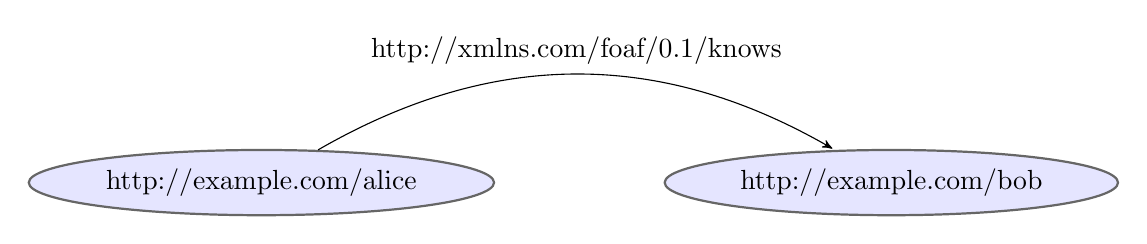
\begin{tikzpicture}[->,>=stealth',shorten >=1pt,auto,thin,
    resource/.style={ellipse,fill=blue!10,draw=black!60,thick},
    literal/.style={fill=white!30,draw}]
    \node[resource] (1) at (0,0) {http://example.com/alice};
    \node[resource] (2) at (8,0) {http://example.com/bob};

    \path[every node/.style={}]
      (1) edge [bend left] node {http://xmlns.com/foaf/0.1/knows} (2);
  \end{tikzpicture}
  \caption{Beispiel eines RDF-Graphs zur Beschreibung einer Beziehung zwischen den Web-Ressourcen Alice und Bob.}
  \label{fig:rdf-simple-graph}
\end{figure}

Die dezentrale Verwaltung von Web-Ressourcen f�hrt zu zwei grundlegenden Problemen. Einerseits kann es vorkommen, dass gleiche Web-Ressourcen unterschiedliche Bezeichner erhalten, andererseits kann es vorkommen, dass f�r unterschiedliche Web-Ressourcen der gleiche Bezeichner verwendet wird. Um dem zweiten Problem entgegenzuwirken, werden im Allgemeinen zur eindeutigen Identifizierung von Web-Ressourcen sogenannte \textit{Uniform Resource Identifiers} (URI, engl. f�r \glqq einheitlicher Bezeichner f�r Ressourcen\grqq) als Indikatoren eingesetzt. Eine URI ist eine Zeichenfolge, die abstrakte oder auch physikalische Ressourcen identifiziert (vgl. \cite{berners2004uniform}).

Wie in Abbildung \ref{fig:rdf-simple-graph} zu sehen ist, werden sowohl Knoten als auch Kanten eines RDF-Graphs mit URIs beschriftet. Bei Literalen sowie sogenannten \textit{Blank Nodes} ist zu ber�cksichtigen, dass diese Regel nicht angewendet wird (vgl. \cite[S.~56-59]{hitzler2007semantic}). Literale sind reservierte Bezeichner f�r RDF-Ressourcen eines bestimmten Datentyps. Im Allgemeinen werden diese Werte durch eine Zeichenkette beschrieben. Der optionale Datentyp gibt dabei an, wie der Datenwert zu interpretieren ist. So beschreiben die Zeichenfolgen \glqq 012{\grqq} und \glqq 12{\grqq} dieselbe nat�rliche Zahl, aber unterschiedliche Zeichenketten. Bei fehlender Angabe eines Datentyps wird das Literal als Zeichenkette interpretiert.

\begin{figure}[h]
  \centering
  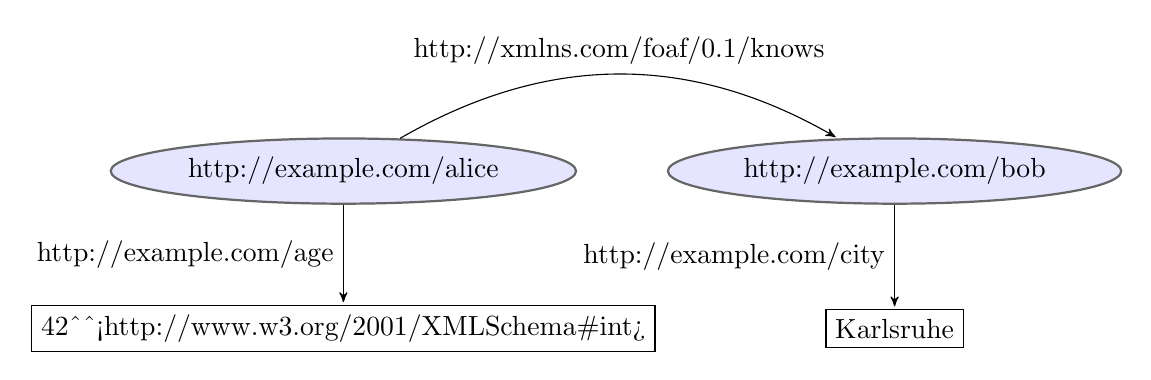
\begin{tikzpicture}[->,>=stealth',shorten >=1pt,auto,thin,
    resource/.style={ellipse,fill=blue!10,draw=black!60,thick},
    literal/.style={fill=white!30,draw}]
    \node[resource] (1) at (0,2) {http://example.com/alice};
    \node[resource] (2) at (7,2) {http://example.com/bob};
    \node[literal] (3) at (0,0) {\glqq 42{\grqq}\^{}\^{}<http://www.w3.org/2001/XMLSchema\#int>};
    \node[literal] (4) at (7,0) {Karlsruhe};

    \path[every node/.style={}]
      (1) edge [bend left] node [] {http://xmlns.com/foaf/0.1/knows} (2)
          edge []          node [left] {http://example.com/age} (3)
      (2) edge []          node [left] {http://example.com/city} (4);
  \end{tikzpicture}
  \caption{Beispiel eines RDF-Graphs mit Literalen und optionalem Datentyp.}
  \label{fig:rdf-literal-graph}
\end{figure}

Abbildung \ref{fig:rdf-literal-graph} zeigt ein einfaches Beispiel eines RDF-Graphs mit Literalen. Nach g�ngiger Konvention werden Ressourcen eines RDF-Graphs durch Ellipsen und Literale durch Rechtecke dargestellt.

\subsection{RDF-Serialisierung}
\label{sub:rdf-syntax}

Wie im vorherigen Abschnitt erl�utert, handelt es sich bei RDF um ein Datenmodell. Zur Beschreibung eines RDF-Graphs k�nnen unterschiedliche Serialisierungen verwendet werden. Die im Allgemeinen verwendeten Notationen werden in diesem Abschnitt kurz erl�utert.

\subsubsection{RDF / XML}

Die Auszeichnungssprache \textit{XML} (E\textbf{x}tensible \textbf{M}arkup \textbf{L}anguage) wird h�ufig f�r einen plattform- und implementierungsunabh�ngigen Austausch von Daten und Informationen zwischen verschiedenen Rechnern mit unterschiedlichen Betriebssystemen verwendet (vgl. \cite{bray1998extensible}). Listing \ref{list:rdf-xml} zeigt das Beispiel aus Abbildung \ref{fig:rdf-literal-graph} in der RDF/XML-Notation.

\begin{minipage}{\linewidth}\hfill
\begin{lstlisting}[language=RDF,caption={Beispiel eines RDF-Dokuments.},label=list:rdf-xml]
<?xml version="1.0" encoding="utf-8" ?>
<rdf:RDF xmlns:foaf="http://xmlns.com/foaf/0.1/" xmlns:ex="http://example.com/"
           xmlns:rdf="http://www.w3.org/1999/02/22-rdf-syntax-ns#">
  <rdf:Description rdf:about="http://example.com/alice">
    <foaf:knows>
      <rdf:Description rdf:about="http://example.com/bob">
        <ex:city>Karlsruhe</ex:city>
      </rdf:Description>
    </foaf:knows>
    <ex:age rdf:datatype="http://www.w3.org/2001/XMLSchema#integer">
      42
    </ex:age>
  </rdf:Description>
</rdf:RDF>
\end{lstlisting}
\end{minipage}

\subsubsection{Turtle}

RDF/XML wurde lange Zeit als Standard-Format zur Beschreibung von RDF-Daten angesehen. Aufgrund der Tatsache, dass XML auf einem Baum- und RDF auf einem Graphen-Modell basiert, wurden im Laufe der Zeit weitere Serialisierungen entwickelt. Eine davon ist die h�ufig verwendete \textit{Turtle}-Notation\footnote{ s. Spezifikation von Turtle unter \url{http://www.w3.org/TeamSubmission/turtle/.}}. Listings \ref{list:rdf-turtle} zeigt das oben dargestellte Beispiel aus Listing \ref{list:rdf-xml} in der Turtle-Notation. URIs werden dabei in spitzen Klammern dargestellt. Jede Aussage wird durch einen Punkt abgeschlossen. Um nicht bei jedem Triple das Subjekt angeben zu m�ssen, k�nnen durch Semikola getrennt weitere Pr�dikate und Objekte angegeben werden. Zus�tzlich gibt es die M�glichkeit, URIs durch die \textit{@prefix}-Syntax einen k�rzeren Namen zu geben und diesen im Dokument anstelle der URI wiederzuverwenden.

\begin{minipage}{\linewidth}\hfill
\begin{lstlisting}[language=Turtle,caption={Turtle-Notation des Beispiels aus Listing \ref{list:rdf-xml}.},label=list:rdf-turtle]
@prefix ex: <http://example.com/> .
@prefix foaf: <http://xmlns.com/foaf/0.1/> .

ex:alice
  foaf:knows ex:bob ;
  ex:age "42"^^<http://www.w3.org/2001/XMLSchema#integer> .
ex:bob ex:city "Karlsruhe" .
\end{lstlisting}
\end{minipage}

Die k�rzere und f�r den Anwender besser lesbare Turtle-Notation wird im Rahmen dieser Abschlussarbeit in allen RDF-Listings verwendet. Aus Gr�nden der �bersichtlichkeit werden die verwendeten Pr�fixe in allen sp�teren Listings nicht explizit angegeben, daf�r aber im Anhang \ref{sec:rdf-prefixe} alphabetisch sortiert aufgelistet.

\subsubsection{N-Triples}
\label{subsub:ntriples}

In diesem Abschnitt wird eine weitere Notation erl�utert, die in der Konzeption und Implementierung des sp�ter vorgestellten ETL-Prozesses ben�tigt wird. \textit{N-Triples}\footnote{ s. Spezifikation von N-Triples unter \url{http://www.w3.org/TR/n-triples/}.} ist eine zeilenbasierte Darstellung eines RDF-Graphs. Jede Zeile repr�sentiert genau ein Triple der Form \glqq <SubjectURI> <PredicateURI> <ObjektURI> .\grqq{}. Der Punkt in der Zeile definiert das Ende der jeweiligen Aussage. Das Beispiel aus Listing \ref{list:rdf-xml} wird in der N-Triples-Notation im Listing \ref{list:rdf-ntriples} dargestellt.

\begin{minipage}{\linewidth}\hfill
\begin{lstlisting}[language=Turtle,caption={N-Triples-Notation des Beispiels aus Listing \ref{list:rdf-xml}.},label=list:rdf-ntriples]
<http://example.com/alice> <http://example.com/age> "42"^^<http://www.w3.org/2001/XMLSchema#integer> .
<http://example.com/alice> <http://xmlns.com/foaf/0.1/knows> <http://example.com/bob> .
<http://example.com/bob> <http://example.com/city> "Karlsruhe" .
\end{lstlisting}
\end{minipage}

Wie in Listing \ref{list:rdf-ntriples} zu erkennen ist, kann der optionale Datentyp eines Literals nach der Zeichenfolge \glqq \textasciicircum\textasciicircum\grqq{} angegeben werden. Auch hier gilt: Ist der Datentyp nicht definiert, wird der Wert des Literals als Zeichenkette interpretiert.

Der Vorteil dieser Notation besteht in der einfachen und zeilenbasierten Darstellung der Triples. Jedes Triple wird in einer einzelnen Zeile beschrieben. Wie im Verlauf der Abschlussarbeit zu sehen sein wird, wird diese Notation bei der Umsetzung des ETL-Prozesses eine entscheidende Rolle spielen. Ein Nachteil dieser Serialisierung besteht jedoch in dem ben�tigten Speicherplatz. Da keine Pr�fixe oder andere M�glichkeiten einer k�rzeren Darstellungsform bestehen, sind in der Regel RDF-Dokumente in der N-Triples-Notation im Vergleich zur Turtle-Notation gr��er.

\subsection{RDF-Schema}
\label{sub:RDF-Schema}

Allein der Einsatz von URIs in RDF erlaubt noch keine semantisch eindeutige Interpretation aller Informationen (vgl. \cite[S.~47-50]{hitzler2007semantic}). Wie bereits im Abschnitt \ref{sub:RDF-Datenmodell} beschrieben, k�nnen gleiche URIs f�r unterschiedliche Ressourcen und unterschiedliche URIs f�r gleiche Ressourcen verwendet werden. Dieser Umstand erzwingt die Verwendung von wohldefinierten Schemata, sogenannte RDF-\textit{Vokabulare}. Unter einem RDF-Schema (RDFS) wird eine Menge von Bezeichnern mit definierter Bedeutung verstanden, die RDF semantisch erweitert und eine Beschreibung benutzerspezifischer Klassen erlaubt (vgl. \cite[S.~66-68]{hitzler2007semantic}).

In den vorangegangenen Abschnitten wurde erl�utert, wie Aussagen �ber Web-Ressourcen get�tigt werden k�nnen, z.\,B. am konkreten Beispiel aus Listing \ref{list:rdf-xml}: \glqq Alice kennt Bob\grqq{}. Durch die Namensgebung \textit{Alice} und \textit{Bob} interpretiert der Anwender den Bezug zu Personen. Maschinen k�nnen nicht ohne Weiteres diesen Bezug herstellen. Die Verwendung von wohldefinierten Vokabularen soll die Interpretation dieser Aussage auch f�r Maschinen erm�glichen.

Im Listing \ref{list:rdf-xml} wird durch die Verwendung des \textit{FOAF}-Vokabulars\footnote{ s. Spezifikation des FOAF-Vokabulars unter \url{http://xmlns.com/foaf/spec/}.} (Friend of a Friend) mit der URI \glqq foaf:knows \grqq{} impliziert, dass es sich hierbei bei Alice und Bob um Personen, also der Klasse \glqq foaf:Person\grqq{} handelt. Wie in vielen Programmiersprachen �blich, beginnen Klassen mit einem Gro�buchstaben und Merkmale mit Kleinbuchstaben.

Das Thema dieser Arbeit behandelt jedoch keine Beziehungen zwischen Personen, sondern die Analyse von statistischen Datens�tzen. In den letzten Jahren hat sich zur Ver�ffentlichung solcher Datens�tze nach dem Linked-Data-Prinzip das RDF Data Cube Vocabulary bew�hrt. Diese werden in den n�chsten Abschnitten genauer betrachtet.

\subsection{Statistical Linked Data}
\label{sub:Statistical-Linked-Data}
Das Linked-Data-Prinzip beschreibt eine Menge von bew�hrten Verfahren f�r das Ver�ffentlichen und Verlinken von strukturierten Daten im Web (vgl. \cite{bizer2009linked}). Die 2006 von Tim Berners-Lee ver�ffentlichte Arbeit \glqq Linked Data: Design Issues\grqq{} \cite{berners2006linkeddata} identifiziert vier Prinzipien f�r die standardisierte Ver�ffentlichung von Daten:

\begin{itemize}
  \item Die frei im Web verf�gbaren Daten werden mit URIs identifiziert.
  \item Das \textit{Hypertext Transfer Protocol} (HTTP) dient zum Auffinden dieser Daten �ber das Web.
  \item Die Verlinkung dieser Daten soll mit etablierten Standards erfolgen, z.\,B. mittels RDF und der graphenbasierten Abfragesprache \textit{SPARQL}\footnote{ s. Spezifikation von SPARQL unter \url{http://www.w3.org/TR/2013/REC-sparql11-overview-20130321/}.} (rekursives Akronym: \textbf{S}PARQL \textbf{P}rotocol \textbf{A}nd \textbf{R}DF \textbf{Q}uery \textbf{L}anguage) (vgl. \cite{perez2006semantics}).
  \item Das Hinzuf�gen von Links zu anderen URIs soll die M�glichkeit bieten, neue Daten und Informationen zu entdecken.
\end{itemize}

In den letzten Jahren ist das Interesse gestiegen, statistische Daten nach dem Linked-Data-Prinzip zu ver�ffentlichen und so die M�glichkeit zu bieten, Daten mit anderen Informationen aus unterschiedlichen Quellen und RDF Stores zu kombinieren. Ein Vorteil besteht hierbei darin, beliebige Zusatzinformationen mit den numerischen Daten verlinken zu k�nnen, um die Bedeutung der Daten n�her zu bestimmen. Wie in Abschnitt \ref{Motivation} bereits erw�hnt k�nnen z.\,B. Provenance-Informationen oder weitergehende Informationen hinzugef�gt werden. Des Weiteren k�nnen auch interne Daten mit den numerischen Daten verlinkt und f�r die Analyse verwendet werden. Diese verlinkten Daten und Informationen werden als \textit{Statistical Linked Data} bezeichnet.

Es existieren verschiedene Vokabulare, die f�r die Ver�ffentlichung statistischer Linked Data in Form von multidimensionalen Cubes verwendet werden k�nnen (vgl. \cite{hausenblas2009scovo}; \cite{vrandecic2010semantics}; \cite{etcheverry2012qb4olap}). Das RDF Data Cube Vocabulary hat sich jedoch weitestgehend durchgesetzt.

\subsection{Das RDF Data Cube Vocabulary}
\label{sub:rdf-data-cube-vocabulary}

Das \textit{RDF Data Cube Vocabulary}\footnote{ s. Spezifikation von QB unter \url{http://www.w3.org/TR/2014/ REC-vocab-data-cube-20140116/}.} (QB) ist ein RDF-Vokabular und ein W3C-Standard zur Beschreibung statistischer Datens�tze in Form von multidimensionalen Cubes (vgl. \cite{zancanaro2013publishing}). Die Ver�ffentlichung von statistischen Daten nach dem Linked-Data-Prinzip sowie die Repr�sentation eines multidimensionalen Datenmodells mit RDF waren die wichtigsten Voraussetzungen bei der Entwicklung des QB-Vokabulars.

Wie im Abschnitt \ref{subsub:olap-datenmodell} bereits erl�utert, bietet das multidimensionale Datenmodell (MDM) eine leicht zu interpretierende Anordnung der statistischer Daten, sodass Analysten einfach und effizient durch den Datenraum navigieren k�nnen. Hauptaugenmerk liegt in der Unterst�tzung der betrieblichen Entscheidungsfindung.

Statistische Daten k�nnen im Bereich Semantic Web mit dem QB-Vokabular beschrieben werden. Abbildung \ref{fig:rdf-qb-vocabulary} veranschaulicht einen Auszug der relevanten Klassen und Beziehungen des Schemata.

\begin{figure}[h]
  \centering
  \includegraphics[width=1\textwidth]{rdf-qb-vocabulary}
  \caption{Wichtigste Klassen und Beziehungen des RDF Data Cube Vokabulars. \newline Quelle: \url{http://www.w3.org/TR/2014/ REC-vocab-data-cube-20140116/}.}
  \label{fig:rdf-qb-vocabulary}
\end{figure}

Der Datensatz (engl. \textit{Dataset}) umfasst die Dimensionen, Measures sowie die Beobachtungen (engl. \textit{Observations}) und Operationen, die mit den Daten ausgef�hrt werden k�nnen. Die wichtigsten Klassen und Beziehungen werden in der folgenden Auflistung n�her erl�utert.

\begin{itemize}
  \item Die Struktur des Cubes wird durch die Klasse \textit{qb:DataStructureDefiniton} (DSD) definiert. Analog zum OLAP-Konzept, bei dem die Daten in Fakten und Dimensionen unterteilt werden, findet bei QB eine Unterteilung der Daten in zwei Bereichen statt. Die erste Unterteilung durch die Property \textit{qb:structure} beschreibt den zugeh�rigen Datensatz des Cubes. Die zweite Unterteilung findet durch die Property \textit{qb:component} statt, welche f�r die Spezifikation der Dimensionen und Measures im Datensatz verantwortlich ist.
  \item \textit{Observations} sind Instanzen von \textit{qb:Observation}. Sie stellen einzelne Beobachtung des Cubes dar und k�nnen aus einem oder mehreren Dimensionen und Measures bestehen. Analog zum OLAP-Konzept beschreibt eine Observation einen Fakt.
  \item Die Klasse \textit{qb:DataSet} stellt die Gesamtmenge der Observations dar. Durch die Verbindung \textit{qb:structure} wird der Bezug zur Datenstruktur definiert.
  \item \textit{qb:DimensionProperty}, \textit{qb:AttributeProperty} und \textit{qb:MeasureProperty} sind vererbte Klassen der \textit{qb:ComponentProperty}-Klasse und repr�sentieren die Dimensionen, Attribute und Measures des Cubes. Analog zum OLAP-Konzept beschreibt die Klasse qb:DimensionProperty die Dimensionen, qb:MeasureProperty die Measures und qb:AttributeProperty zus�tzliche Attribute des Cubes.
  \item Im OLAP-Kontext besitzt jeder Fakt in der Regel einen Bezug zu einer konkreten Instanzen einer Dimensionen. Diese als Member bezeichnete Beziehung kann im QB-Vokabular entweder explizit, durch die Eigenschaft \textit{qb:codeList}, oder implizit durch das Vorkommen in den Fakten beschrieben werden.
  \item In QB werden Hierarchien durch die Klasse \textit{skos:ConceptScheme} und die Levels durch \textit{skos:Concept} repr�sentiert. Der Bezug eines Levels zu einer Hierarchie wird durch die Property \textit{skos:inScheme} definiert. Der Bezug zu einer konkreten Instanz einer Dimension wird durch die Property \textit{skos:member} bestimmt. Die Vater-Kind-Beziehung \textit{skos:narrower} erm�glicht die Navigation zwischen den Levels (vgl. \cite{kampgen2011transforming}).
\end{itemize}

In einem OLAP Cube wird in der Regel f�r jedes Measure eine Aggregationsfunktion definiert, wie z.\,B. \textit{sum}, \textit{min}, \textit{max}, \textit{avg} und \textit{count}. In QB gibt es keine Beschreibung dieser Aggregationsfunktionen f�r Measures. Daher wird in dieser Arbeit zur Beschreibung der Measures das QB4O-Vokabular\footnote{ s. Spezifikation von QB4O unter \url{http://purl.org/qb4olap/cubes\#}.} mit der Property \textit{qb4o:aggregateFunction} verwendet. Dies erm�glicht den Einsatz der URIs f�r die Aggregationsfunktionen \textit{qb4o:sum}, \textit{qb4o:min}, \textit{qb4o:max}, \textit{qb4o:avg} und \textit{qb4o:count}.

F�r die Analyse einer enorm gro�en Datenmenge sind Technologien aus dem Big-Data-Bereich notwendig. Diese werden im n�chsten Kapitel einer Beschreibung unterzogen.

\section{Big Data}
\label{Big-Data}

Es existieren unz�hlige Definitionen von Big Data (vgl. \cite[S.~34-37]{king2014big}). Die anerkannteste Definition charakterisiert Big Data anhand von drei bis vier Kriterien (vgl. \cite{laney20013d}; \cite[S.~35]{king2014big}; \cite[S.~7-8]{dorschel2015praxishandbuch}): \glqq Volume\grqq{}, \glqq Velocity\grqq{}, \glqq Variety\grqq{} und gegebenenfalls \glqq Veracity\grqq{}.

\begin{description}
  \item[Volumen (Volumne)] \hfill \\
  Die gro�e Menge an Daten ist der wesentlichste Aspekt von Big Data. Das anfallende Datenvolumen der zu verarbeitenden Informationen steigt stetig an. Ein Grund hierf�r sind z.\,B. kleine und immer leistungsf�higere Computerchips, die in viele Lebensbereiche vordringen und neue Daten generieren. Dies f�hrt zu einer anwachsenden Datenmenge, die bei der Analyse genutzt werden soll.
  \item[Geschwindigkeit (Velocity)] \hfill \\
  Dieses Merkmal wird nicht immer eindeutig interpretiert. Zum einen wird hierunter die Geschwindigkeit verstanden, mit der neue Daten entstehen (vgl. \cite[S.~7]{dorschel2015praxishandbuch}; \cite{fasel2014big}). Andererseits kann Velocity auch die Geschwindigkeit beschreiben, mit der Daten verarbeitet werden m�ssen (vgl. \cite[S.~35]{king2014big}).
  \item[Vielfalt (Variety)] \hfill \\
  Das Merkmal Variety kennzeichnet die Heterogenit�t der Daten. Die zunehmende Anzahl an Datenquellen, die f�r die Analyse herangezogen werden, kann zu stark variierenden oder gar unbekannten Datenstrukturen f�hren. Ferner sind f�r Big Data viele der relevanten Daten unstrukturiert. Auch in solchen F�llen sollen Analysen m�glich sein und zu neuen Erkenntnissen f�hren.
  \item[Richtigkeit (Veracity)] \hfill \\
  Dieses Merkmal wird in einigen Big-Data-Definitionen als viertes Merkmal angesehen (vgl. \cite{bendler2014taming}; \cite[S.~35]{king2014big}). Diese Eigenschaft bezieht sich auf die Qualit�t der Daten bezogen auf die Richtigkeit und Vollst�ndigkeit. Bevor betriebliche Entscheidungen getroffen werden k�nnen, muss die Korrektheit und die Relevanz der Daten zum Zeitpunkt der Analyse bekannt sein.
\end{description}

In der Regel �bersteigen eine solche Datenmenge und die f�r die Analyse verwendeten Prozesse die Speicher- und Verarbeitungskapazit�t eines einzelnen Rechners. Aus diesem Grund hat sich in den letzten Jahren die Verwendung von \textit{Rechner-Clusters}\footnote{ Ein Cluster wird als Verbund von mehreren vernetzten Computern bezeichnet.} etabliert. Eine solche Architektur wurde dazu optimiert, eine Berechnung, eine Analyse oder ein Programm verteilt auf verschiedenen Rechnern parallel auszuf�hren. Die Eigenschaften einer solchen Architektur k�nnen in drei Bereiche zusammengefasst werden (vgl. \cite[S.~279]{dorschel2015praxishandbuch}; \cite[S.~65-66]{rahm2015verteiltes}):

\begin{description}
  \item[Parallele Verarbeitung der Daten] \hfill \\
  Die Sicherstellung einer konstanten Verarbeitungszeit bei steigendem Datenvolumen durch verteilte Parallelverarbeitung muss gew�hrleistet sein. Durch die Speicherung der Daten auf lokalen Festplatten vieler Rechnerknoten soll eine Verarbeitung der Daten jeweils auf den Knoten durchgef�hrt werden, auf denen die Daten gespeichert wurden. Dies erlaubt einen gleichzeitig stattfindenden und unabh�ngigen Datenzugriff auf die Daten einzelner Rechner. Diese als \textit{Shared Nothing} bezeichnete Architektur soll eine lineare Skalierbarkeit garantieren, die praktisch unbegrenzt ist (vgl. \cite[S.~55-58]{rahm2015verteiltes}).
  \item[Horizontale Skalierung] \hfill \\
  Bei Bedarf kann durch Hinzuf�gen von neuen Rechnern die Kapazit�t des Clusters erweitert werden. Dieser Vorgang wird als horizontale Skalierung bezeichnet. Zur Vermeidung hoher Hardware-Kosten soll die M�glichkeit bestehen, das Cluster durch Rechner mit gew�hnlicher Hardware (engl. \textit{Commodity Hardware}) bereitzustellen und zu erweitern.
  \item[Redundante Speicherung] \hfill \\
  Zum Zweck der Fehlertoleranz und f�r eine Verbesserung der Antwortzeiten sollen die Daten auf mehrere Rechnerknoten repliziert und redundant gespeichert werden. Bei Ausfall eines Rechners kann der entsprechende Prozess auf einem anderen Rechnerknoten fortgesetzt werden. Zur Vermeidung eines inkonsistenten Systems m�ssen daher Daten�nderungen auf alle Replikate �bertragen werden. Ein weiterer Vorteil wird in der Ausf�hrung eines Prozesses deutlich, indem ein Rechner mit hoher Last durch einen Rechner mit niedriger Last ersetzt werden kann.
\end{description}

Sowohl relationale Datenbanken, RDF Stores als auch OLAP Engines skalieren in der Regel nicht horizontal. Sie besitzen eine nat�rliche Grenze bzgl. ihrer Datenspeicher- und Datenverarbeitungskapazit�t (vgl. \cite[S.~260-262]{dorschel2015praxishandbuch}). Bei der Analyse gro�er Datenmengen sind daher Big-Data-Technologien mit den oben definierten Eigenschaften notwendig. Mit Apache Hadoop sind derartige Technologien in einem Open Source Software Stack verf�gbar.

\subsection{Das Apache-Hadoop-Framework}
F�r die verteilte Parallelverarbeitung gro�er Datenmengen hat sich Apache Hadoop\footnote{ s. Webseite des Apache Hadoop Projekts unter \url{http://hadoop.apache.org/}.} als Standard etabliert\footnote{ s. Apache Hadoop PowerdBy unter \url{http://wiki.apache.org/hadoop/PoweredBy}.}. Apache Hadoop ist ein quelloffenes und in Java entwickeltes Top-Level-Projekt der Apache Software Foundation.

Die Hauptkomponenten von Apache Hadoop bestehen aus dem Hadoop Distributed File System und dem Programmiermodell MapReduce. In den nachfolgenden Abschnitten werden diese Komponenten einer n�heren Betrachtung unterzogen.

\subsection{Das verteilte Dateisystem von Apache Hadoop: HDFS}
\label{sub:hdfs}
Das \textit{Hadoop Distributes Files System} (HDFS) ist ein verteiltes Dateisystem, welches von Googles 2003 vorgestellte \textit{Googles File System} \cite{ghemawat2003google} inspiriert wurde (vgl. \cite{shafer2010hadoop}). Die wichtigsten Ziele des Entwurfs lagen in der Fehlertoleranz bei Commodity-Hardware-Umgebungen, in der Ausrichtung gro�er Datenmengen und in der parallelen Batch-Verar-beitung dieser Daten. Letzteres bezweckt einen hohen Lesedurchsatz anstelle von niedrigen Latenzen. Zus�tzlich basiert die Umsetzung von HDFS auf der Annahme, dass Daten oft gelesen, aber selten bis gar nicht ver�ndert werden (das sogenannte \textit{write-once-read-many}-Prinzip, vgl. \cite[S.~66-69]{rahm2015verteiltes}).

HDFS baut auf einer Master-Slave-Architektur auf, bestehend aus dem Masterknoten \mbox{\textit{NameNode}} und mehreren \textit{DataNodes}. Der NameNode ist f�r die Verwaltung des Dateisystems sowie f�r den Dateizugriff des Clients verantwortlich. Der NameNode unterst�tzt eine Vielzahl von Operationen, wie z.\,B. das �ffnen, Schlie�en und Umbenennen von Dateien und Verzeichnissen. Die DataNodes dagegen sind f�r die Speicherung und Verwaltung der Daten zust�ndig. Bei der Speicherung der Daten im HDFS findet zun�chst eine Aufteilung der Dateien in Datenbl�cke statt. Diese Bl�cke werden �ber die verschiedenen DataNodes horizontal verteilt. Die Gr��e des Blocks kann bei jedem Upload in das HDFS und pro Datei einzeln festgelegt werden (Standardwert ist 128 MB). Ferner kann pro Datei ein Replikationsfaktor definiert werden. Dieser Wert gibt die Anzahl der Replikationen von jedem einzelnen Block im HDFS an. Standardgem�� werden bei Apache Hadoop drei Replikationen angelegt. Die Zuordnung zwischen DataNode und Block erfolgt durch den NameNode. Zur Veranschaulichung der HDFS-Architektur dient die Abbildung \ref{fig:hdfs}.

\begin{figure}[h]
  \centering
  \includegraphics[width=0.85\textwidth]{hdfs}
  \caption{Architektur von HDFS und Beispiel einer Leseoperation in Anlehnung an \cite[S.~67]{rahm2015verteiltes} und \cite[S.~280]{dorschel2015praxishandbuch}.}
  \label{fig:hdfs}
\end{figure}

Die Matainformationen zur Verzeichnisstruktur und weitergehende Informationen (z.\,B. welcher Block wurde auf welchem DataNode gespeichert?) werden in dem lokalen Hauptspeicher des NameNodes gespeichert (vgl. \cite[S.~67]{rahm2015verteiltes}). Ferner werden alle �nderungsvorg�nge in das lokale Dateisystem �bertragen, um jederzeit einen nachvollziehbaren Ablauf der ausgef�hrten Operationen zu gew�hrleisten.

Die Registrierung eines neuen DataNodes erfolgt �ber eine \textit{Heartbeat}-Message (vgl. \cite{shafer2010hadoop}). Zudem steht der NameNode in st�ndigem Kontakt mit allen Rechnern des Clusters. So wird gew�hrleistet, dass ein DataNode seiner Funktion nachkommen kann. Wird diese Nachricht in einer bestimmten Zeitspanne nicht �bermittelt, geht der NameNode von einem Ausfall des Rechners aus und f�hrt Ma�nahmen zur Neuverteilung der verlorenen Bl�cke auf die restlichen DataNodes durch.

Da ein NameNode einen \textit{Single-Point-of-Failure} darstellt, ist es �blich, bei Ausfall des NameNodes die Verf�gbarkeit des Dateisystems durch einen zweiten NameNode sicherzustellen, dem sogenannten \textit{Secondary NameNode} (s. Abbildung \ref{fig:hdfs}).

Der Ablauf von Operationen ist bei HDFS fest vordefiniert. Wie in Abbildung \ref{fig:hdfs} dargestellt, kontaktiert der Client, z.\,B. bei einer Lese-Operation, zuerst den NameNode. Dieser liefert eine Liste mit allen DataNodes, die eine Replikation der ben�tigten Bl�cke aufweisen. Anschlie�end kontaktiert der Client die DataNodes direkt an, um die Bl�cke der ben�tigten Dateien anzufordern.

Die Replikation der Datenbl�cke im HDFS dient nicht nur dem Zweck der Fehlertoleranz und der Ausfallsicherheit, wie der n�chste Abschnitt zeigen soll.

\subsection{Parallele Ausf�hrung mit dem Programmiermodell MapReduce}
\label{sub:mapreduce}
\textit{MapReduce} ist ein von Google 2004 vorgestelltes Programmiermodell f�r die parallele Verarbeitung gro�er, unstrukturierter oder semi-strukturierter verteilter Datens�tze in Rechner-Clustern (vgl. \cite{dean2004mapreduce}). Aufgrund der Einfachheit, Ausfallsicherheit und hohen Flexibilit�t hat das MapReduce-Modell eine weite Verbreitung erfahren, vor allem durch die frei verf�gbare Implementierung in Apache Hadoop.

Das Hauptziel einer MapReduce-Funktion liegt darin, ein definiertes Problem in mehrere Teilaufgaben, sogenannte \textit{Map-Task}, zu zerlegen, diese �ber die Rechner eines Clusters f�r die parallele Berechnung zu verteilen und die Zwischenergebnisse innerhalb des Clusters auszutauschen. Nach Beendigung der Berechnungen werden die Zwischenergebnisse durch sogenannte \textit{Reduce-Tasks} aggregiert und zu einem Endergebnis zusammengefasst (vgl. \cite[S.~280-281]{dorschel2015praxishandbuch}). Eine parallele Ausf�hrung ist m�glich, da die Prozesse zur Berechnung der Ergebnisse zu den verarbeitenden Daten bewegt werden.

\begin{figure}[h]
  \centering
  \includegraphics[width=0.9\textwidth]{mapreduce}
  \caption{Gesamtablauf eines MapReduce-Jobs in Apache Hadoop, angelehnt an \cite[S.~69]{rahm2015verteiltes}.}
  \label{fig:mr}
\end{figure}

�hnlich wie HDFS basiert auch die MapReduce-Engine von Apache Hadoop auf der Master-Slave-Architektur. Ein auszuf�hrender MapReduce-Prozess, ein sogenannter \textit{Job}, wird vom Master-Knoten, dem sogenannten \textit{JobTracker}-Knoten, in mehrere \textit{Tasks} zerlegt. Der JobTracker dient als Koordination- und Kontroll-Komponente eines MapReduce-Jobs und weist, nach der Zerlegung des Jobs in mehrere Tasks, diese den sogenannten \textit{Worker}-Knoten zu. Zudem steht der JobTracker-Knoten in st�ndigem Kontakt mit den Worker-Knoten. So soll sichergestellt werden, dass abgebrochene Tasks erneut ausgef�hrt werden. Abbildung \ref{fig:mr} veranschaulicht den Gesamtablauf eines MapReduce-Prozesses in Hadoop.

Grundlegendes Ziel bei der Ausf�hrung eines MapReduce-Jobs ist die Zuweisung eines Task an einen Worker-Knoten, der im HDFS den f�r den Prozess notwendigen Block gespeichert hat. Dies f�hrt zu einem lokalen Lesezugriff. Wurde der ben�tigte Datenblock zuvor nicht lokal gespeichert, muss dieser zuerst �ber HDFS angefordert und lokal gespeichert werden.

Die Aufgabe einer MapReduce-Funktion besteht darin, eine gro�e Datenmenge von \textit{Key-Value}-Paaren zusammenzufassen und auf eine kleinere Menge von Key-Value-Paaren zu reduzieren. Hierbei bilden die zwei Funktionen \textit{Map} und \textit{Reduce} die Hauptkomponenten der Berechnung.
\begin{align*}
map(key_{in}, value_{in}) & \rightarrow [(key^1_{tmp},value^1_{tmp}), \dots , (key^n_{tmp}, value^n_{tmp})]\\
reduce([(key^s_{tmp}, [value^t_{tmp}, \dots , value^u_{tmp}])]) & \rightarrow [(key^q_{out}, value^q_{out}), \dots , (key^p_{out}, value^p_{out})]
\end{align*}

Ein wesentlicher Schritt eines MapReduce-Jobs ist die \textit{Shuffle}-Phase. Voraussetzung f�r die Ausf�hrung eines Reduce-Tasks ist die Sortierung der Ergebnisse eines Map-Tasks nach ihrem Key und dem Zusammenfassen der berechneten Values in eine Liste (vgl. \cite[S.~70]{rahm2015verteiltes}).

Nachdem in der Shuffle-Phase das Ergebnis des Map-Tasks sortiert und auf der Festplatte des Workers gespeichert wurde, wird der Reduce-Task angesto�en. Dabei findet anhand der Keys eine Aggregierung der Values statt. Anschlie�end wird das Ergebnis in eine HDFS-Datei gespeichert. Da es sich bei einem Worker-Knoten auch gleichzeitig um ein DataNode handelt, wird das Ergebnis entsprechend der Erl�uterung im vorangegangenen Abschnitt \ref{sub:hdfs} horizontal verteilt und repliziert.

\subsubsection{MapReduce - Beispiel}

In diesem Abschnitt soll das MapReduce-Programmiermodell anhand eines Beispiels erl�utert werden. Analog zu HelloWorld-Programmen gibt es bei MapReduce das \textit{Word-Count}-Beispiel. Hierbei sollen in einem Text die Anzahl der W�rter ermittelt werden. Abbildung \ref{fig:mr-example-word-count} dient dabei der Veranschaulichung.

\begin{figure}[h]
  \centering
  \includegraphics[width=0.95\textwidth]{mp-example-word-count}
  \caption{Word-Count-Beispiel eines MapReduce-Jobs mit drei Map- und drei Reduce-Tasks, eigene Darstellung.}
  \label{fig:mr-example-word-count}
\end{figure}

Die Eingabe besteht aus einer Text-Datei mit einem beliebigen Inhalt. Durch die Speicherung im HDFS wird die Datei in drei Datenbl�cke unterteilt und auf die Rechner des Cluster verteilt. Der Map-Task transformiert jedes Wort in ein Key-Value-Paar. Beispielsweise k�nnte die Map-Phase die Eingabe wie folgt umwandeln:
\begin{align*}
map(sentence_1, \text{\glqq Hello World Bye World\grqq{}}) & \rightarrow [ (\text{hello}, 1), (\text{world}, 2), (\text{bye}, 1) ]\\
map(sentence_2, \text{\glqq Hello Hadoop Bye Bye\grqq{}}) & \rightarrow [ (\text{hello}, 1), (\text{hadoop}, 1), (\text{bye}, 2) ]\\
map(sentence_3, \text{\glqq Hello MR Goodbye MR\grqq{}}) & \rightarrow [ (\text{hello}, 1), (\text{mr}, 2), (\text{goodbye}, 1) ]
\end{align*}
Die Shuffle-Phase sortiert die berechneten Paare nach ihrem Key in alphabetischer Reihenfolge und fasst die berechneten Values in einer Liste zusammen. Dieses Ergebnis dient als Eingabe der Reduce-Funktionen. Der Reduce-Job hat die Aufgabe, die Elemente in der Liste zu z�hlen und in einem Wert zu aggregieren.
\begin{align*}
reduce([(\text{bye}, [ 1, 2 ]), (\text{goodbye}, [ 1 ])]) & \rightarrow [ (\text{bye}, 3), (\text{goodbye}, 1) ]\\
reduce([(\text{hadoop}, [ 1 ]), (\text{hello}, [ 1, 1, 1 ])]) & \rightarrow [ (\text{hadoop}, 1), (\text{hello}, 3) ]\\
reduce([(\text{mr}, [ 2 ]), (\text{world}, [ 2 ])]) & \rightarrow [ (\text{mr}, 2), (\text{world}, 2) ]
\end{align*}
Die Ausgabe der Reduce-Funktionen wird zu einem Endergebnis zusammengefasst und in einer Datei im HDFS gespeichert.

Im diesem Abschnitt wurde das Konzept des MapReduce-Programmiermodells an einem Beispiel erl�utert. Die Entwicklung von MapReduce-Jobs erfordert f�r unternehmensspezifische Analysen zur Entscheidungsfindung jedoch spezialisierte Software-Entwickler. Diese Prozesse sind bei �nderungen schwierig zu pflegen. Ferner ist ein Umzug eines bestehenden MapReduce-Jobs in einen neuen oder �hnlichen Kontext in der Regel nicht leicht umzusetzen. Aus diesem Grund wird im n�chsten Abschnitt Apache Hive vorgestellt.

\subsection{Apache Hadoops Data Warehouse: Apache Hive}
\label{sub:hive}
Apache \textit{Hive}\footnote{ s. Webeite von Apache Hive unter \url{https://hive.apache.org/}.} ist eine 2009 von Facebook ver�ffentlichte Open Source Data-Warehousing-L�sung f�r Apache Hadoop (vgl. \cite{thusoo2009hive}, s. Abbildung \ref{fig:hive}). �hnlich wie bei relationalen Datenbanken werden die Daten in tabellarischer Form mit Spalten und Zeilen dargestellt, wobei die Daten im HDFS gespeichert und horizontal verteilt werden. Diese Daten lassen sich mit der zugeh�rigen SQL-�hnlichen Abfragesprache \textit{HiveQL} (Hive Query Language) abfragen. HiveQL unterst�tzt neben primitiven Datentypen wie z.\,B. Strings, Integer und Boolean auch Mengen (engl. \textit{Collections}) wie Arrays, Maps und verschachtelte Kombinationen beider Datenstrukturen (vgl. \cite{thusoo2010hive}). Eine HiveQL-Abfrage wird bei der Ausf�hrung automatisch in ein oder mehreren MapReduce-Jobs kompiliert und auf Apache Hadoop ausgef�hrt. Zus�tzlich ist es m�glich, benutzerspezifische MapReduce-Skripte in die Abfragen zu integrieren.

\begin{figure}[h]
  \centering
  \includegraphics[width=0.7\textwidth]{hive}
  \caption{Architektur von Apache Hive auf Basis von Apache Hadoop in Anlehnung an \cite{thusoo2009hive}.}
  \label{fig:hive}
\end{figure}

Die zugrundeliegende I/O-Bibliotheken in Hive erlauben unterschiedliche Datenstrukturen. So ist es m�glich, zeilenbasierte Textdateien wie CSV-Dateien oder komprimierte Dateien, wie z.\,B. im Avro\footnote{ s. Apache Avro Dokumentation unter \url{http://avro.apache.org/docs/current/}.}- oder Parquet\footnote{ s. Apache Parquet Dokumentation unter \url{https://parquet.apache.org/documentation/latest/}.}-Format, im HDFS abzulegen und mit HiveQL abzufragen.

F�r die Speicherung der Metainformationen von Hive-Tabellen ist der sogenannte \textit{Hive-Metastore} zust�ndig. In der Regel wird hierf�r eine relationale Datenbank wie MySQL verwendet. Dieser Katalog speichert neben dem Hive-Schemata (Welche Hive-Tabellen existieren? Welche Spalten enthalten die Hive-Tabellen? Welchen Datentyp haben die Spalten? Welches Datenformat wird verwendet?) auch zus�tzlich statistische Datenwerte (Wie viele Eintr�ge besitzt die Hive-Tabelle? Wie viel Speicherplatz wird verbraucht?), die bei der Abfrage-Optimierung und Generierung der MapReduce-Jobs ben�tigt werden (vgl. \cite{thusoo2009hive}; \cite{thusoo2010hive}).

Ein gro�er Vorteil von Apache Hive ist die m�gliche Anbindung mittels eines JDBC\footnote{ JDBC steht f�r Java Database Connection. Sie definiert eine einheitliche Schnittstelle (API) zu Datenbanken unterschiedlichster Hersteller.}-Treibers, welcher in dieser Abschlussarbeit bei der Umsetzung des ETL-Prozesses eine wesentliche Rollen spielen wird. Zus�tzlich wird in der Konzeption der Wide Column Store Apache HBase eine wichtige Funktion haben. Dies ist Gegenstand des n�chsten Abschnitts.

\subsection{Apache Hadoops Datenbank: Apache HBase}
\label{sub:hbase}

Apache \textit{HBase}\footnote{ s. Webseite von Apache HBase unter \url{http://hbase.apache.org/}.} ist eine von Googles \textit{BigTable} \cite{chang2006bigtable} inspirierte, spaltenorientierte, fehlertolerante und horizontal skalierbare Datenbank auf Basis von HDFS. Sie z�hlt zu den sogenannten \textit{NoSQL}-Datenbanksystemen\footnote{ NoSQL (Not only SQL) bezeichnet Datenbanken, die einen nicht-relationalen Ansatz verfolgen und in der Regel nicht mit der Abfragesprache SQL abgefragt werden k�nnen.} (vgl. \cite[S.~457]{george2011hbase}).

�hnlich wie bei relationalen Datenbanken basiert das Datenmodell von HBase auf Tabellen. Eine HBase-Tabelle besteht aus Zeilen und Spalten. Eine Zeile beschreibt einen Datensatz, w�hrend eine Spalte ein Attribut repr�sentiert. Entsprechend einem Prim�rschl�ssel in relationalen Datenbanken erfolgt jeder Zugriff auf eine Zeile in HBase durch einen nicht ver�nderbaren und eindeutigen Schl�ssel (engl. \textit{Row Key}). HBase verwendet f�r den Row Key ein Byte-Array, wodurch dem Entwickler bei der Definition eines Schl�ssels viel Spielraum geboten wird (vgl. \cite[S.~66]{redmond2012sieben}).

Spalten k�nnen zur Laufzeit hinzugef�gt werden. Leere Zeilen existieren in HBase nicht. Das Anlegen einer Zeile findet nur dann statt, wenn sie einen Wert besitzt. Zus�tzlich werden die Zeilen versioniert. Aus diesem Grund f�gt HBase bei Einf�geoperationen automatisch einen Zeitstempel (engl. \textit{Timestamp}) hinzu.

Ein wichtiges Unterscheidungsmerkmal von HBase im Vergleich zu relationalen Datenbanken ist das Datenschema. Das Datenschema in HBase wird durch eine Tabelle, eine Spaltenfamilie (engl. \textit{Column Family}) und deren Eigenschaft festgelegt. Die Column Family ist ein von Googles BigTable �bernommenes Konzept (vgl. \cite{chang2006bigtable}; \cite[S.~66]{redmond2012sieben}). Die Daten einer Column Family werden physisch zusammenh�ngend gespeichert. Dies f�hrt bei Abfragen zu k�rzeren Ausf�hrungszeiten. Aus diesem Grund erm�glicht HBase zuf�llige Lese- und Schreiboperationen in Echtzeit f�r gro�e Datenmengen (vgl. \cite{redmond2012sieben}).

Der Zugriff auf eine Spalte erfolgt �ber den Verbund zwischen der Column Family und dem Bezeichner der Spalte in Form von $[Column Family]:[Spaltenbezeichner]$. Eine Column Family muss vorab als Teil des Schemata einer HBase-Tabelle definiert sein. Spalten k�nnen zu jedem Zeitpunkt zu einer Column Family hinzugef�gt werden, solange diese existiert.

Das zugrundeliegende Datenmodell von HBase ist ein assoziatives Array\footnote{ Ein assoziatives Array wird auch als \textit{Map} oder \textit{Dictionary} bezeichnet.}. Die Zeilen k�nnen wiederum auch als ein assoziatives Array gesehen werden (Row Key $\rightarrow$ Column Family). Die Werte der Column Family werden ebenfalls als assoziatives Array betrachtet. Aus diesem Grund wird das Datenmodell von HBase als ein mehrdimensionales assoziatives Array bezeichnet.

�hnlich wie Apache Hadoop baut Apache HBase auf einer Master-Slave-Architektur auf. Der zentrale Master-Knoten, der sogenannte \textit{MasterServer}, �berwacht die Slave-Knoten, die in HBase als \textit{RegionServer} bezeichnet werden. Der MasterServer �bernimmt die Verteilung der Daten auf die verschiedenen RegionServer. Diese wiederum stellen den Datenzugriff sicher und �bernehmen die Speicherung der Daten ins HDFS. Abbildung \ref{fig:hbase-architektur} zeigt ein Beispiel eines Clusters mit mehreren RegionServer.

\begin{figure}[h]
  \centering
  \includegraphics[width=0.85\textwidth]{hbase}
  \caption{Architektur von HBase, angelehnt an \cite[S.~79]{redmond2012sieben}.}
  \label{fig:hbase-architektur}
\end{figure}

Zu Beginn werden die Daten einer HBase-Tabelle in einer einzelnen \textit{Region} gespeichert. �berschreitet die Datenmenge einen definierbaren Schwellwert, wird die Region durch den MasterServer automatisch in zwei neue Regionen mit gleicher Gr��e geteilt und auf die verf�gbaren RegionServer �bertragen. Aufgrund der Sortierung der Datens�tze nach dem Row Key kann zu jedem Zeitpunkt der RegionServer ermittelt werden, der die ben�tigten Daten lokal gespeichert hat.

Im Gegensatz zum Masterknoten in HDFS und MapReduce �bernimmt Apache \mbox{Zookeeper}\footnote{ s. Apache Zookeeper Webseite unter \url{https://zookeeper.apache.org/}.} die Funktionen und Aufgaben wie die Synchronisation, die Konfiguration und die Ausfallsicherheit von HBase (vgl. \cite{hunt2010zookeeper}). Zookeeper ist eine Koordinierungsstelle f�r verteilte Systeme und vereinfacht die Umsetzung und �berwachung von verteilten Anwendungen.

HBase bietet einen wahlfreien Zugriff auf extrem gro�e Datenmengen und eignet sich besonders gut als horizontal skalierende Datenbank zur Datenhaltung mehrerer Milliarden Datens�tze (vgl. \cite[S.~80]{redmond2012sieben}). Aus diesem Grund wird HBase im Rahmen dieser Abschlussarbeit von besonderer Bedeutung sein.

  \chapter{Konzeption}
\label{cha:Konzeption}
In den letzten Jahren ist das Interesse gestiegen, statistische Daten nach dem Linked-Data-Prinzip zu ver�ffentlichen\footnote{ s. Linked Data Webseite unter \url{http://linkeddata.org/}.}. Dieses Konzept bietet die M�glichkeit, Daten mit zus�tzlichen Informationen aus unterschiedlichen Quellen im Web zu verkn�pfen.

F�r die Analayse statistscher Datens�tze werden h�ufig Konzepte aus der Business Intelligence eingesetzt. Dabei werden die zu analysierenden Daten aus unterschiedlichen, heterogenen operativen Systemen mithilfe eines ETL-Prozesses bereinigt, Konflikte aufgel�st und in ein Data Warehouse gespeichert. Zur Unterst�tzung der betrieblichen Entscheidungsfindung unterst�tzt das Konzept OLAP die Analyse der konsolidierten Daten mit verschiedenen Operationen, die eine interaktive Navigation durch den Datenraum erm�glichen.

Die Analyse von Statistical Linked Data mit OLAP scheint ein vielversprechender Ansatz zur Unterst�tzung der Entscheidungsfindung zu sein. In einer fr�heren Publikation \glqq Transforming Statistical Linked Data for Use in OLAP Systems\grqq{} \cite{kampgen2011transforming} von K�mpgen und Harth wurde ein ETL-Prozess vorgestellt, der Statistical Linked Data im QB-Vokabular aus einer RDF-Datenbank in ein multidimensionales Datenmodell transformiert. Aufgrund der Metainformationen im QB-Vokabular war es m�glich, die RDF-Daten automatisiert in eine relationale Datenbank im Sternschema zu speichern und f�r OLAP-Abfragen  bereitzustellen.

Bei diesem Ansatz stellt sich jedoch die Frage, wie eine enorm gro�e Menge an Statistical Linked Data effizient analysiert werden kann? Sowohl die relationale als auch die RDF-Datenbank skalieren in diesem ETL-Prozess nicht horizontal und besitzen daher eine nat�rliche Grenze bzgl. ihrer Datenspeicher- und Datenverarbeitungskapazit�t. Dies resultiert in einer sehr langen Ausf�hrungsdauer des ETL-Prozesses zur Bef�llung der relationalen Datenbank im Sternschema. Zus�tzlich ist die Ausf�hrung interaktiver Analysen von gro�en Datenmengen bei relationalen Datenbanken nicht effizient genug, da bereits ein einfaches Scannen der Daten zu einer hohen zeitlichen Latenz f�hrt.

F�r Analysen gro�er Datenmengen sind daher Technologien aus dem Big-Data-Umfeld notwendig, die die Beschr�nkungen klassischer Systeme mittels Parallelisierung �ber viele Rechner hinweg �berwinden. Mit Apache Hadoop sind derartige Technologien in einem Open Source Software Stack verf�gbar.

In diesem Kapitel werden die verwendeten Technologien und deren Zusammenspiel, sowie die Idee, das Konzept und die geplante Architektur genauer betrachtet. Ziel ist es, einen L�sungsansatz zu pr�sentieren, der das von K�mpgen und Harth \cite{kampgen2011transforming} vorgestellte Konzept in eine horizontal skalierende Architektur auf der Basis von Apache Hadoop �berf�hrt.

\section{Verwendete Technologien}
Bevor auf die einzelnen Komponenten und deren Zusammenspiel in der Architektur eingegangen wird, sollen die in der Konzeption verwendeten Technologien genauer beschrieben werden. �hnlich zur Herangehensweise bei der Definition des Begriffs \glqq Business Intelligence\grqq{} in Kapitel \ref{sec:konzepte-und-prozesse} wird im ersten Abschnitt \ref{sub:kylin} ein Projekt aus der Datenbereitstellungsschicht in Form von Apache Kylin vorgestellt. In Abschnitt \ref{sub:mondrian} wird das Open-Source-Projekt Mondrian aus der Analyseschicht einer n�heren Betrachtung unterzogen.

\subsection{Apache Kylin}
\label{sub:kylin}
Vor der Ver�ffentlichung von \textit{Apache Kylin}\footnote{ s. Apache Kylin Webseite unter \url{http://kylin.incubator.apache.org/}.} im Jahr 2014 war es im Open-Source-Bereich nicht ohne weiteres m�glich, auf Basis von Apache Hadoop das OLAP-Konzept f�r interaktive Abfragen auf Grundlage einer beliebig gro�en Datenmenge effizient umzusetzen. Es wurden zwar einige Arbeiten zum Thema \textit{OLAP-on-Hadoop} ver�ffentlicht, die sich weder in der Praxis noch in der Wissenschaft etablieren konnten (vgl. \cite{chevalier2015implementing}; \cite{weidner2013fast}; \cite{zhang2013olap}; \cite{Abello}; \cite{arres2013building}).

Die von eBay im Oktober 2014 ver�ffentlichte OLAP-Engine Apache Kylin zeigt einen interessanten Ansatz, um die in der klassischen Business Intelligence seit vielen Jahren etablierten OLAP Cubes mit Unterst�tzung der Hadoop-Plattform in die Big-Data-Welt zu �bertragen. Der Einsatz von Kylin wird durch etablierte Open-Source-Projekte aus dem Hadoop-�kosystem beg�nstigt, die seit vielen Jahren von einer Vielzahl von Unternehmen produktiv eingesetzt werden.

Die folgende Abbildung \ref{fig:kylin-architektur} stellt das Zusammenspiel der Hadoop-Komponenten in Kylins Architektur dar. Dabei ist zwischen einem \textit{Offline}- und \textit{Online}-Datenfluss zu unterscheiden.

\begin{figure}[h]
  \centering
  \includegraphics[width=0.85\textwidth]{kylin-architektur}
  \caption{Kylin-Architektur mit Komponenten aus dem Hadoop-�kosystem, in Anlehnung an \url{http://kylin.apache.org/}.}
  \label{fig:kylin-architektur}
\end{figure}

\begin{description}
  \item[Offline-Datenfluss] \hfill \\
  Die Generierung des OLAP Cubes setzt die Speicherung der Daten im HDFS und die Modellierung dieser Daten in Apache Hive als Sternschema voraus. Zus�tzlich werden Metainformationen ben�tigt, welche die Cube-Struktur und die sp�ter m�glichen OLAP-Abfragen beschreiben. Im Offline-Datenfluss (blauer Pfad in Abbildung \ref{fig:kylin-architektur}) greift die \textit{Cube Build Engine} auf diese Metainformationen zu und generiert mit mehreren, hintereinander ausgef�hrten HiveQL-Abfragen die Cuboids. Durch die �bersetzung der HiveQL-Abfragen in MapReduce-Jobs findet eine parallele Verarbeitung statt (s. Abschnitt \ref{sub:hive}).

  F�r die Speicherung der Cuboids wird die NoSQL-Datenbank HBase verwendet. Im nicht-relationalen, spaltenorientierten und verteilten Wide Column Store werden die vorberechneten Aggregationen der verschiedenen Cuboids gespeichert und �ber das Cluster hinweg horizontal verteilt (s. vorangehender Abschnitt HBase \ref{sub:hbase}).

  Kylin bietet die M�glichkeit, den Offline-Pfad f�r neu hinzukommende Daten inkrementell auszuf�hren. Dies kann in beliebigen Zeitabschnitten erfolgen, wie z.\,B. jede Stunde, einmal am Tag oder einmal im Monat. Mit dieser Eigenschaft wird im Rahmen der Abschlussarbeit das in der Einleitung vorgestellte Problem (V3) untersucht.
  \item[Online-Datenfluss] \hfill \\
  Nach der erfolgreichen Generierung des OLAP Cubes stehen die Daten f�r die Analysen zur Verf�gung. Der Online-Datenfluss (gr�ner Pfad in Abbildung \ref{fig:kylin-architektur}) beschreibt die Interaktion mit Kylin. Dabei werden SQL-Anfragen entweder direkt �ber die REST-Schnittstelle oder mithilfe der mitgelieferten Treiber und einem SQL-basierten BI-Tool an den REST\footnote{ REST steht f�r \textit{Representational State Transfer} und beschreibt ein zustandsloses Client-Server-Protokoll �ber HTTP. }-Server gesendet.

  In der SQL-Query-Engine schreibt Apache Calcite\footnote{ s. Apache Calcite Webseite \url{http://calcite.apache.org/}} die SQL-Abfrage in HBase Requests um. Wurden die angefragten Daten im HBase Cube vorberechnet, k�nnen die SQL-Abfragen, durch die horizontale Speicherung der Cuboids mit einer Ausf�hrungszeitn im (Sub-)Sekundenbereich beantwortet werden. Das entspricht dem \textit{Low-Latency-Pfad} in Abbildung \ref{fig:kylin-architektur} (gr�ner, durchgezogener Pfad).

  Sind die angeforderten Daten der SQL-Abfrage nicht vorberechnet, kann das SQL-Statement an Apache Hive weitergeleitet werden. Hierbei wandelt Hive die Query in MapReduce-Jobs um, deren Abarbeitung mit einem entsprechenden Overhead und Latenzen verbunden ist (s. MapReduce Abschnitt \ref{sub:mapreduce}). Das entspricht der Ausf�hrung der SQL-Anfrage im \textit{Mid-Latency-Pfad} (gr�ner, gestrichelter Pfad). Je nach Datenmenge eignet sich der Vorgang nur eingeschr�nkt f�r interaktive Analysen.
\end{description}

Das wesentliche Ziel von Kylin besteht darin, f�r m�glichst viele Abfragen des Nutzers den Low-Latency-Pfad bereitzustellen. Aus diesem Grund sind w�hrend der Definition des OLAP Cubes die Anforderungen der Analysten f�r die betriebliche Entscheidungsfindung bestm�glich zu ber�cksichtigen.

\subsubsection{Definition des OLAP-Datenmodells in Kylin}
\label{subsub:kylin-datenmodell}
Kylin setzt f�r die Generierung des OLAP Cubes die Abbildung der Daten in Apache Hive im Sternschema voraus. Bevor mit der eigentlichen Daten-Modellierung des OLAP Cubes begonnen werden kann, sind die Tabellen aus dem Hive Metastore mit Kylin zu synchronisieren. Dabei werden im Hintergrund Metainformationen zu den Hive-Tabellen erstellt und in eine eigens daf�r vorgesehene HBase-Tabelle gespeichert. Dadurch stehen der Modellierung des OLAP Cubes alle notwendigen Informationen zur Verf�gung, wie beispielsweise die Spaltennamen der Dimensionstabellen oder die Datentypen der Measures. Erst nach dieser Synchronisierung kann die Daten-Modellierung des Cubes Schritt f�r Schritt interaktiv in der Weboberfl�che oder mit der daf�r vorgesehenen REST-Schnittstelle mit einem JSON Request aufgebaut werden.

Der erste Schritt besteht in der Definition des OLAP-Datenmodells. Nach Auswahl der Faktentabelle sind die Dimensionstabellen zu definieren und um Angaben der \textit{Primary}- und \textit{Foreign Keys} zu erg�nzen.

Die Beschreibung der Dimensionen findet anhand von drei unterschiedlichen Typen statt: \textit{Normal}, \textit{Hierarchy} und \textit{Derived}. Bei der Auswahl \glqq Normal\grqq{} wird die Dimension ohne jede Besonderheit zum Cube hinzugef�gt. Beim Typ \glqq Hierarchy\grqq{} bietet Kylin eine hierarchische Anordnung der Attribute einer Dimension an. Wie bereits in Abschnitt \ref{subsub:olap-functions} beschrieben, spielt diese Art der Anordnung der Daten eine wichtige Rolle f�r die Drill-down- und Roll-up-Navigation durch den Cube. Die letzte M�glichkeit, eine Dimension hinzuzuf�gen, besteht im Typ \glqq Derived\grqq{}. Hierbei handelt es sich um Attribute einer Dimension, die keinem hierarchischen Aufbau entsprechen und sich eindeutig durch einen Primary Key ableiten lassen. Die Berechnung der Measures basiert folglich lediglich auf diese einzelnen Keys. Das f�hrt zu einer Reduktion der Kombinationsm�glichkeiten der Dimensionen, da nicht jede m�gliche Zusammenstellung der Spaltenwerte ber�cksichtig werden.

Zus�tzlich zu den Dimensionen m�ssen die Measures des OLAP Cubes definiert werden. Die Auswahl der Aggregationsfunktionen ist zum Zeitpunkt der Abschlussarbeit auf \textit{SUM}, \textit{MIN}, \textit{MAX}, \textit{COUNT} und \textit{COUNT\_DISTINCT} beschr�nkt.

Optional k�nnen sogenannte \textit{Refresh Settings} definiert werden. Dies erm�glicht OLAP Cubes mit neu hinzukommenden Daten zu generieren und mit bestehenden Cubes zu vereinen. Hierbei ist eine Date-Spalte im Format \glqq YYYY-MM-DD\grqq{} auszuw�hlen und ein Startdatum anzugeben.

Kylin bietet zudem die M�glichkeit, erweiterte Einstellungen zu definieren, die eine Optimierung des Cubes erm�glichen. Bei einer gro�en Anzahl an Dimensionen ist es nicht sinnvoll, jedes Cuboid zu berechnen. Beispielsweise w�ren bei 30 Dimensionen $2^{30}$ (etwas mehr als eine Milliarde) Cuboids zu erstellen. Mit \textit{Aggregation Groups} kann eine Unterteilung dieser 30 Dimensionen in Gruppen durchgef�hrt und so ein Partial Cube definiert werden (s. Abschnitt \ref{subsub:molap}). Statt $2^{30}$ Cuboids zu generieren, kann der Cube beispielsweise in drei Gruppen � 10 Dimensionen aufgeteilt werden. Die Anzahl der Cuboids reduziert sich dadurch auf $2^{10} + 2^{10} + 2^{10}$ (= 3072 Cuboids). Sowohl die Berechnungszeit der Aggregationen als auch der Speicherverbrauch des OLAP Cubes werden hierdurch deutlich reduziert. Bei ung�nstiger Wahl der Aggregation Groups kann jedoch ein fehlendes Cuboid die Ausf�hrungszeit der Analyse stark beeintr�chtigen (s. Mid-Latency-Pfad in Abbildung \ref{fig:kylin-architektur}).

\subsubsection{Der Cube Build Process}
\label{subsub:kylin-cube-build-process}
Nach erfolgreicher Modellierung des OLAP Cubes ist die Ausf�hrung des \textit{Cube-Build}-Prozesses m�glich. Anhand der Metainformationen und der Datenmodellierung werden die Aggregate in den verschiedenen Kombinationsm�glichkeiten der Dimensionen berechnet. Abbildung \ref{fig:kylin-cube-build} stellt den Workflow dar.

\begin{figure}[h]
  \centering
  \includegraphics[width=1\textwidth]{kylin-cube-build}
  \caption{Kylins Cube-Build-Prozess als Workflow.}
  \label{fig:kylin-cube-build}
\end{figure}

Im ersten Teil des Prozesses wird ein \textit{Dictionary} angelegt. Das Dictionary wird bei Dimensionen verwendet, die keine gro�e Kardinalit�t besitzen. In solch einem Fall speichert Kylin bei der Generierung des OLAP Cubes nicht den eigentlichen Wert in die HBase-Datenbank, sondern eine Referenz zum Dictionary. Diese Einstellung kann pro Spalte der Dimensionstabellen individuell angegeben werden.

Im n�chsten Abschnitt des Prozesses werden alle verwendeten Hive-Tabellen des OLAP Cubes zun�chst in einer \textit{Intermediate Hive Table} zusammengefasst. Dabei wird in einer einzelnen HiveQL-Abfrage die Faktentabelle mit allen Dimensionstabellen in der Intermediate Hive-Tabelle vereint und gespeichert. Diese Tabelle dient als Grundlage f�r die Generierung des gr��tm�glichen N-Cuboids (vgl. Abbildung \ref{fig:cuboids} in Abschnitt \ref{subsub:molap}). Durch verschiedene Gruppierungen werden mithilfe mehrerer hintereinander ausgef�hrter MapReduce-Jobs die immer kleiner werdenden Cuboids berechnet, bis der 0-Cuboid ermittelt wird. Ein ausreichend gro�er Speicherplatz im HDFS ist zwingend erforderlich, da alle Zwischenergebnisse als \textit{HDFS Sequence Files} abgelegt werden.

Sind die Cuboids berechnet, werden die Zwischenergebnisse in einem letzten MapReduce-Job in eine \textit{HFile} transformiert. HFiles sind Dateien im HDFS, die HBase f�r die Datenspeicherung verwendet. Der letzte Schritt besteht im Importieren dieser HFile in HBase in Form eines \textit{Bulk-Load}-Prozesses.

Je nach Gr��e der Datenmenge und der Anzahl der Knoten des Clusters kann der Build-Prozess einige Zeit beanspruchen. Anschlie�end sind die Vorbereitungen f�r die Verarbeitung analytischer OLAP Queries abgeschlossen.

\subsubsection{Vor- und Nachteile von Kylin}

Die Vorteile von Apache Kylin sind vielf�ltig. Es handelt sich um den ersten erfolgreichen Versuch, OLAP-Funktionalit�ten auf Apache Hadoop aufzusetzen. Zudem basiert das Open-Source-Projekt aufgrund der Verwendung von HDFS, Hive, MapReduce, HBase und Calcite auf Systemen aus dem Hadoop-�kosystem, die sich in den letzten Jahren etabliert haben. Der produktive Einsatz von Kylin bei eBay zeigt das Potenzial des Projektes. Die M�glichkeit der horizontalen Skalierung im Cube-Build-Prozess sowie die horizontale Verteilung der Cuboids durch HBase f�hrt dazu, dass Kylin enorm gro�e Datens�tze verarbeiten und die vorberechneten Daten f�r Analysen effizient bereitstellen kann.

Ein wesentlicher Nachteil besteht jedoch in der eingeschr�nkten Abfragem�glichkeit: Kylin kann ausschlie�lich SQL-Abfragen interpretieren. Aus diesem Grund wird im n�chsten Abschnitt Pentahos MDX-to-SQL Engine Mondrian vorgestellt.

\subsection{Pentaho Mondrian}
\label{sub:mondrian}
MDX ist eine Abfragesprache, welche h�ufig bei komplexen OLAP-Operationen gew�hlt wird (s. Abschnitt \ref{sub:mdx}). Aus diesem Grund setzen viele OLAP Client MDX als Standardsprache ein. Neben dem Vorteil der erweiterten Selektierbarkeit besteht eine weitere St�rke von MDX darin, mit Roll-Up- und Drill-Down-Operationen durch Hierarchien entlang eines Pfades zu navigieren. Jedoch ist die Anzahl der Datenbanken, die MDX interpretieren und verarbeiten k�nnen, gering. Infolgedessen wurde bereits 2001 das Projekt Mondrian\footnote{ s. Pentaho Mondrian Webseite unter \url{http://community.pentaho.com/projects/mondrian/}.} begonnen - ein quelloffener, in Java entwickelter OLAP Server (vgl. \cite[S.~3]{back2013mondrian}). Auf der einen Seite wollen Analysten MDX-Abfragen f�r ihre Analysen nutzen, auf der anderen Seite jedoch nicht auf die einfache Anwendung und Nutzung von relationalen Datenbanken verzichten. Um auf die Daten einer relationalen Datenbank mit MDX zuzugreifen, muss eine Umwandlung der MDX-Abfragen in SQL stattfinden. Diese Transformation war eines der wichtigen Ziele bei der Entwicklung von Mondrian.

Ein weiteres Ziel bei der Entwicklung von Mondrian bestand darin, interaktive Analysen von gr��ere Datenmengen zu erm�glichen. Die relationalen Daten m�ssen daher im Sternschema angeordnet sein. Zus�tzlich wurde in Mondrian ein Cache implementiert, der aus bereits ausgef�hrten SQL-Abfragen einen multidimensionalen OLAP Cube erstellt, um nachfolgende MDX-Abfragen direkt �ber den Cube im Cache beantworten oder das Ergebnis ableiten zu k�nnen. Abbildung \ref{fig:mondrian-architektur} zeigt ein typisches Ablaufdiagramm in Mondrian.

\begin{figure}[h]
  \centering
  \includegraphics[width=0.70\textwidth]{mondrian-architektur}
  \caption{Ablaufdiagramm von Mondrian bei der Ausf�hrung einer MDX-Abfrage, in Anlehnung an \cite[S.~12]{back2013mondrian}.}
  \label{fig:mondrian-architektur}
\end{figure}

Die MDX-Abfragen k�nnen entweder �ber einen OLAP Client wie Saiku\footnote{ s. Saiku Webseite \url{http://www.meteorite.bi/products/saiku}.} oder direkt �ber einen API Call, z.\,B. mit der Java-Bibliothek OLAP4J\footnote{ s. OLAP4J Webseite \url{http://www.olap4j.org/}.}, an den Mondrian-Server gesendet werden. Nach Validierung der MDX-Abfrage wird �berpr�ft, ob das Ergebnis mit Hilfe von zuvor ausgef�hrten MDX-Abfragen und durch Speicherung der Ergebnisse als OLAP Cube im Cache beantwortet werden kann. Falls dies m�glich ist, wird das Ergebnis direkt aus dem Cache abgeleitet und als MDX Result Set zur�ck an den OLAP Client gesendet. Kann die Abfrage nicht aus den Daten im Cache abgeleitet werden, werden unter Zuhilfenahme des Mondrian Schema eine Folge von SQL-Anfragen generiert und an das Data Warehouse gesendet. Die Einzelresultate werden zu einem Ergebnisse aggregiert, zusammengefasst und im Cache in einer multidimensionalen Struktur als Cube gespeichert, sodass dieses Ergebnis bei sp�teren Abfragen wiederverwendet werden kann. Der letzte Schritt besteht im Zur�cksenden des von Mondrian ermittelten Resultats als MDX Result Set an den OLAP Client.

Mondrian operiert in der Regel mit klassischen relationalen Datenbanken wie MySQL oder PostgreSQL. Die Beziehungen zwischen den relationalen und den multidimensionalen Strukturen werden im sogenannten \textit{Mondrian Schema} definiert. Diese in XML beschriebene Konfigurationsdatei gibt die Tabellen und Spalten des relationalen Datenbankschemas an und definiert die Faktentabelle als auch die Dimensionstabellen des multidimensionalen OLAP Cubes. Zus�tzlich werden alle Measures des Cubes, die verwendeten Aggregationsfunktionen, Hierarchien in den Dimensionen mit ihren Levels und Attributen im Mondrian Schema deklariert.

Ferner kann Mondrian durch \textit{SQL Dialects} erweitert werden, um die Kommunikation mit anderen Datenbanken zu erm�glichen, die SQL-Abfragen oder zumindest eine Teilmenge davon interpretieren k�nnen. Ein weiteres Ziel der vorliegenden Arbeit wird daher in der Implementierung eines Kylin Dialects bestehen, die die Beantwortung von MDX-Abfragen in Apache Kylin realisieren soll.

\section{Idee und Aufbau der Architektur}

Der eingangs in Abschnitt \ref{Zielsetzung} beschriebene ETL-Prozess von K�mpgen und Harth \cite{kampgen2011transforming} transformiert die Statistical Linked Data einer RDF-Datenbank durch mehrere, hintereinander ausgef�hrten SPARQL-Abfragen in ein multidimensionales Datenmodell. Aufgrund der Metainformationen im QB-Vokabular ist es m�glich, die RDF-Daten automatisiert in eine relationale Datenbank im Sternschema zu speichern und f�r OLAP-Abfragen bereitzustellen.

Wie bereits erl�utert, sind Technologien aus dem Big-Data-Umfeld f�r die Analyse einer enorm gro�en Datenmenge notwendig. Der hier pr�sentierte L�sungsansatz �berf�hrt daher K�mpgen und Harths ETL-Prozess in eine horizontal skalierende Architektur auf der Basis von Apache Hadoop. Die nicht-skalierbaren Komponenten, wie die RDF-Datenbank, die Abfragesprache SPARQL und die relationale Datenbank werden dabei durch Technologien und Frameworks aus dem Hadoop-�kosystem ersetzt. Abbildung \ref{fig:etl-architektur} veranschaulicht die neue Gesamtarchitektur. Die Hauptziele bestehen darin, die Ausf�hrungsdauer zur Beladung des Data Warehouses sowie die Antwortzeiten analytischer OLAP-Abfragen auch bei einem beliebig gro�en Datenvolumen zu reduzieren.

\begin{figure}[h]
  \centering
  \includegraphics[width=1\textwidth]{etl-architektur}
  \caption{Parallelisierungsarchitektur des ETL-Prozesses mit MapReduce zur Bewirtschaftung der RDF-Daten im QB-Vokabular in Apache Kylin.}
  \label{fig:etl-architektur}
\end{figure}

F�r die Umsetzung der Architektur ist neben einem funktionierenden Apache Hadoop Cluster auch eine fehlerfreie Installation von Apache Kylin auf einem Cluster-Knoten notwendig. Im Rahmen dieser Arbeit wird Kylin auf dem Master-Knoten installiert.

Die Umsetzung des ETL-Prozesses besteht aus f�nf Komponenten, wie in Abbildung \ref{fig:etl-architektur} dargestellt wird. Die Konzeptionen der einzelnen Komponenten sowie deren Aufgaben werden in den n�chsten Abschnitten beschrieben.

\subsection{Komponente 1: Umzug der RDF-Daten nach Hive}
Wie bereits im Abschnitt \ref{sub:rdf-data-cube-vocabulary} beschrieben, beinhalten RDF-Daten, die durch das QB-Vokabular beschrieben werden, neben den eigentlichen statistischen Daten zus�tzliche Metainformationen, die die Struktur des OLAP Cubes beschreiben. Die statistischen Linked Data m�ssen f�r die sp�ter stattfindende parallele Ausf�hrung des ETL-Prozesses in das Hadoop-�kosystem umgezogen werden.

Vor dem Umzug der RDF-Daten ins HDFS muss eine Transformation stattfinden. Die durch verschiedene Syntaxen beschriebenen RDF-Daten werden in das zeilenbasierte N-Triples-Format umgewandelt. Dies hat folgende Gr�nde:
\begin{itemize}
\item Das einfache N-Triples-Format enth�lt pro Zeile genau ein Triple der Form Subjekt, Pr�dikat und Objekt. Durch diese einfache Struktur ist es m�glich, die Hive-Tabelle QB\_Triples mit drei Spalten (\textit{subject}, \textit{predicate}, \textit{object}) zu generieren.
\item Aufgrund der Speicherung im HDFS werden die Daten in Datenbl�cke mit einer bestimmten Gr��e aufgeteilt, horizontal �ber die verschiedenen Datanodes des Clusters verteilt und repliziert (s. Abschnitt \ref{sub:hdfs}). Ein nicht-zeilenbasiertes Format k�nnte dazu f�hren, dass ein Triple �ber mehrere Zeilen in zwei unterschiedliche Datenbl�cke getrennt wird. Dies w�rde zu fehlenden Triples und einem fehlerhaften Verhalten beim Auslesen der Triples f�hren.
\end{itemize}

Folglich ist es notwendig, die RDF-Daten vor dem Umzug in das HDFS in das zeilenbasiertes N-Triples-Format umzuwandeln. Nach dieser Transformation und dem Umzug ins HDFS kann die Hive-Tabelle \textit{QB\_Triples} durch eine \textit{Create-HiveQ}L-Abfrage erstellt werden. Ziel der RDF-2-Hive-Komponenten ist es, der n�chsten Komponente \textit{MDM-Loader} die M�glichkeit zu bieten, die Struktur des OLAP Cubes aus den RDF-Daten im QB-Vokabular mit mehreren, hintereinander ausgef�hrten HiveQL-Abfragen aus der Hive-Tabelle QB\_Triples auszulesen.

\subsection{Komponente 2: Auslesen des multidimensionalen Models}
Nach Generierung der Hive-Tabelle QB\_Triples werden mithilfe von verschiedenen, hintereinander ausgef�hrten HiveQL-Abfragen die Metainformationen aus dem RDF im QB-Vokabular ausgelesen. Diese Aufgabe �bernimmt die zweite Komponente \textit{MDM-Loader}. Die Abfragen haben das Ziel, alle Cube-Informationen mit effizienten HiveQL-Abfragen auszulesen. Die Definition geeigneter HiveQL-Abfragen und der daraus entstehenden MapReduce-Jobs f�hrt zur parallelen Verarbeitung der Abfragen �ber die Cluster-Knoten. Dabei werden die Measures, Dimensionen, Hierarchien, Levels, Attribute und Fact Members des OLAP Cubes aus einer beliebig gro�en Menge an RDF-Daten ermittelt.

Grundlegendes Ziel ist eine geeignete Repr�sentation des Datenmodells. Zudem werden in dieser Komponente bereits Metainformationen definiert und Vorbereitungen f�r die darauffolgenden Schritte get�tigt. Wie bereits im Abschnitt \ref{subsub:kylin-datenmodell} dargestellt, m�ssen die Daten f�r Kylin in Hive im Sternschema vorliegen. Folglich werden bereits anhand der ausgelesenen Informationen aus dem MDM die Tabellen- und Spaltennamen der Faktentabelle und der Dimensionstabellen generisch bestimmt. Zudem beinhaltet das MDM alle erforderlichen Metainformationen wie die Datentypen sowie Primary-Key- und Foreign-Key-Zuweisungen des Sternschemas.

Ausgehend vom MDM und den ausgelesenen Metainformationen aus den RDF-Daten im QB-Vokabular werden die restlichen drei Komponenten ausgef�hrt.

\subsection{Komponente 3: Generierung des Sternschemas in Hive}
\label{sub:komp3}
Alle relevanten Daten m�ssen vor der Generierung des OLAP Cubes in Hive-Tabellen im Sternschema modelliert werden. Demnach ist eine Transformation der Hive-Tabelle QB\_Triples in Hive-Tabellen des Sternschemas notwendig. Hive bietet die M�glichkeit, eine neue Tabelle aus bereits bestehenden Tabellen durch einen HiveQL-Statement zu generieren. Solche Abfragen werden im Hive-Kontext als \textit{CTAS}-Statements (Create Table As Select) bezeichnet. F�r die Generierung des Sternschemas werden durch die zuvor ausgelesenen Informationen aus der QB\_Triples-Tabelle die Fakten- und alle Dimensionstabellen erstellt. Die Schwierigkeit liegt darin, das zeilenbasierten Format der QB\_Triples-Tabelle (jede Zeile repr�sentiert ein Triple, eine konkrete Instanz einer Dimension kann mehrere Attribute und dadurch mehrere Zeilen lang sein) in ein spaltenorientiertes Format umzuwandeln (jede Zeile repr�sentiert ein Objekt, die Spalten stellen die Attribute dar).

\subsection{Komponente 4: Metadata Modell und Cube Build in Kylin}
Der REST-Server von Kylin bietet, neben der M�glichkeit SQL-Abfragen auszuf�hren, noch weitere Funktionen an. Die dritte Komponente \textit{MDM-2-Kylin} nutzt diese M�glichkeit, um folgende REST Requests auszuf�hren:
\begin{description}
  \item[Optional: Neues Projekt erstellen] \hfill \\
  Bevor der OLAP Cube generiert werden kann, ist optional ein neues Projekt in Kylin anzulegen. Neben dem Namen des Projekts ist auch die Angabe einer Beschreibung m�glich.
  \item[Synchronisation] \hfill \\
  Die Synchronisation der Hive-Tabellen in Kylin erfolgt durch einen einfachen REST Request. �hnlich zum Hive-Metastore werden hierbei Informationen �ber die synchronisierten Tabellen generiert und in einer daf�r speziell vorgesehene HBase-Tabelle gespeichert.
  \item[OLAP-Datenmodell definieren] \hfill \\
  Nach der Synchronisierung werden die Metainformationen des zu generierenden OLAP-Datenmodells mit einem weiteren REST Request an Kylin �bermittelt. Aus diesem Grund ist eine Transformation des zuvor ausgelesenen MDMs in ein JSON-Format notwendig. Kylin ben�tigt folgende Metainformationen f�r den Cube Designer:

  \begin{itemize}
    \item Deklaration der Faktentabelle in Hive.
    \item Festlegung der Hive-Tabellen, die die Dimensionstabellen des OLAP Cubes repr�sentieren. Zus�tzliche Informationen beinhalten den Join-Typ (\textit{Inner}-, \textit{Left}-, \textit{Right}-Join) und die Join-Bedingung (\textit{Foreign-Key}- und \textit{Primary-Key}-Zuweisung).
    \item Informationen �ber den Aufbau der einzelnen Dimensionen: Hierarchien, Levels, und Attribute. Zudem sind Dimensionen, die durch eine Spalte in der Faktentabelle definiert werden, ebenfalls anzugeben.
    \item Deklaration der Measures des OLAP Cubes durch Angabe des Datentyps, der Aggregationsfunktion und der zugeh�rigen Spalte der Faktentabelle.
    \item Optionale Definition von Refresh-Settings und Aggregation Groups (s. Erl�uterung in Abschnitt \ref{subsub:kylin-datenmodell}).
  \end{itemize}
  \item[Cube-Build-Prozess ansto�en] \hfill \\
  Die dritte Aufgabe der MDM-2-Kylin-Komponente besteht darin, den Cube-Build-Prozess �ber den REST-Server zu starten. Aufgrund der Dauer des Prozesses soll der aktuelle Stand in einem definierten Intervall abgefragt und dem Benutzer mitgeteilt werden.
\end{description}

\subsection{Komponente 5: Mondrian Schema definieren}

Die letzte Komponente hat die Aufgabe, aus den Informationen des MDMs ein Mondrian Schema zu generieren. Diese XML-Konfigurationsdatei wird in Mondrian ben�tigt, um die MDX-Abfragen des OLAP Clients in ein f�r Kylin verst�ndliches SQL umzuwandeln (s. Abschnitt \ref{sub:mondrian}). Hierbei findet eine Transformation des MDMs in das XML-Format statt. Nach diesem Schritt ist der ETL-Prozess beendet.

\section{Ziele der Architektur}
Erst nach erfolgreichem Abschluss der f�nf Komponenten ist es m�glich, die Daten entweder mit MDX-Abfragen �ber einen OLAP Client wie Saiku mit Mondrian, �ber die SQL REST-Schnittstelle in Kylin oder �ber ein SQL-basiertes BI-Tool wie Tableau\footnote{ s. Webseite von Tableau unter \url{http://www.tableau.com/de-de/business-intelligence}.} und dem JDBC-Treiber abzufragen.

Die Dauer des ETL-Prozesses richtet sich nach der Menge der zu verarbeitenden Daten und der Anzahl der Cluster-Knoten. Eine Hypothese dieser Abschlussarbeit liegt in der �berpr�fung, ob die parallele Ausf�hrung durch die hintereinander ausgef�hrten HiveQL-Abfragen und der Generierung von MapReduce-Jobs einen Vorteil gegen�ber nicht horizontal skalierenden ETL-Prozessen mit sich bringt?

Ein weiteres Ziel liegt in der Reduzierung der Ausf�hrungsdauer bei analytischen OLAP-Abfragen. In Abh�ngigkeit der Clustergr��e soll durch die horizontale Speicherung der Cuboids in HBase die Abfragedauer auch bei einer beliebig gro�en Datenmenge im Sekundenbereich liegen.

Nach der Definition des Konzepts wird im n�chsten Kapitel die Implementierung, der technische Aufwand, die dabei entstandenen Probleme sowie die verwendeten HiveQL-Abfragen einer genaueren Betrachtung unterzogen.

  \chapter{Implementierung}
\label{cha:Implementierung}

In diesem Kapitel wird auf die technische Implementierung sowie auf die Anforderungen des ETL-Prozesses detailliert eingegangen. Zun�chst wird in Abschnitt \ref{sec:kylin-kommunikation} die entwickelte Kommunikationsm�glichkeit zwischen Apache Kylin und Pentaho Mondrian durch einen SQL-Dialekt f�r die Ausf�hrung von MDX-Abfragen behandelt. Anschlie�end werden die im vorherigen Kapitel definierten Komponenten des ETL-Prozesses auf technischer Ebene anhand eines abstrakten Beispiels verdeutlicht. Die Anforderungen, die entstandenen Probleme mit ihren L�sungsans�tzen sowie weitergehende Optimierungsm�glichkeiten werden in den folgenden Abschnitten beschrieben.

\section{Kommunikation zwischen Apache Kylin und Mondrian}
\label{sec:kylin-kommunikation}
Mondrian �bersetzt MDX-Abfragen in SQL-Statements f�r unterschiedliche relationale sowie nicht-relationale Datenbanken. Zum Zeitpunkt der Abschlussarbeit existiert jedoch kein SQL-Dialekt f�r die Generierung von SQL-Abfragen f�r Apache Kylin. Wie bereits im Abschnitt \ref{sub:kylin} beschrieben, kann Kylin durch die Integration von Apache Calcite eine ANSI-SQL-Teilmenge interpretieren. Daher werden viele SQL-Abfragen erfolgreich in HBase Requests umgesetzt, einige wenige wie z.\,B. implizit angegebenen Joins bleiben jedoch nicht ausf�hrbar. Listing \ref{list:kylin-join-implicit} zeigt ein einfaches Beispiel einer SQL-Abfrage, die von Kylin nicht ausgef�hrt werden kann.

\begin{minipage}{\linewidth}\hfill
\begin{lstlisting}[language=SQL,caption={Beispiel einer SQL-Anfrage mit impliziten Join.},label=list:kylin-join-implicit]
-- Join-Anfrage, die von Kylin nicht unterst�tzt wird
SELECT *
FROM Fact, Dim1
WHERE Fact.dim1_id = Dim1.id;
\end{lstlisting}
\end{minipage}

Demnach m�ssen Joins durch das SQL-Schl�sselwort \textit{JOIN} und der direkt darauffolgenden \textit{ON}-Bedingung deklariert werden (s. Listing \ref{list:kylin-join-explicit}).

\begin{minipage}{\linewidth}\hfill
\begin{lstlisting}[language=SQL,caption={Beispiel einer SQL-Anfrage mit expliziten Join.},label=list:kylin-join-explicit]
-- Join-Anfrage, die von Kylin unterst�tzt wird
SELECT *
FROM Fact
JOIN Dim1 ON Fact.dim1_id = Dim1.id;
\end{lstlisting}
\end{minipage}

Zudem unterst�tzt Kylin keine \textit{Distinct Counts}. Die Integration von Mondrian in Kylin setzt daher ein SQL-Dialekt voraus, welcher f�r Kylin verst�ndliche SQL-Abfragen generiert.

\subsection{Kylin SQL-Dialekt in Mondrian erstellen}

Mondrian stellt Methoden bereit, um mit einem SQL-Dialekt das gew�nschte SQL-Statement zu generieren. Das in Listing \ref{list:kylin-join-implicit} vorgestellte Implicit-Join-Problem kann durch die Methode aus Listing \ref{list:kylin-sql-dialekt-join} gel�st werden.

\begin{minipage}{\linewidth}\hfill
\begin{lstlisting}[language=Java,caption={Generierung von expliziten SQL-Joins durch die Methode \textit{allowsJoinOn()}.},label=list:kylin-sql-dialekt-join]
public boolean allowsJoinOn() {
  return true;
}
\end{lstlisting}
\end{minipage}

Der Einsatz des Kylin Dialekts erwies sich bei der Umsetzung in Mondrian 3 als fehlerhaft. Die Methode \textit{allowsJoinOn()} wurde bei der Generierung der SQL-Abfragen nicht ber�cksichtigt. Dieser Fehler wurde in Mondrian 4 behoben. Folglich wurde f�r den weiteren Verlauf der Abschlussarbeit Mondrian 4 verwendet.

\begin{minipage}{\linewidth}\hfill
\begin{lstlisting}[language=Java,caption={Deaktivierung der \textit{DISTINCT COUNT}-Methode im Kylin-SQL-Dialekt durch die Methode \textit{allowsCountDistinct()}.},label=list:kylin-sql-dialekt-count]
public boolean allowsCountDistinct() {
  return false;
}
\end{lstlisting}
\end{minipage}

Die n�chste zu implementierenden Methode in Kylins Dialect ist \textit{allowsCountDistinct()}, die \textit{false} als R�ckgabewert hat (s. Listing \ref{list:kylin-sql-dialekt-count}), da Kylin zum Zeitpunkt der Arbeit solch eine Count-Abfrage nicht unterst�tzt.

\section{Implementierung der ETL-Komponenten}

F�r die Entwicklung des ETL-Prozesses wurde die Programmiersprache Java gew�hlt. Mithilfe des JDBC-Treibers von Apache Hive wird der Zugriff auf die QB\_Triples-Tabelle und die Generierung der Hive-Tabellen im Sternschema erm�glicht. %Die Ausf�hrung des ETL-Prozesses muss dabei direkt auf einem der Knoten des Rechner-Clusters ausgef�hrt werden. Zus�tzlich ist vor dem Start zu �berpr�fen, ob der Benutzer die notwendigen Rechte besitzt, im HDFS neue Ordner und in Hive neue Tabellen anzulegen.

Zum besseren Verst�ndnis wird dieser technische Abschnitt anhand eines abstrakten Beispiels beschrieben. Zur Veranschaulichung dient die Abbildung \ref{fig:qb-graph-example}. Die zu analysierenden RDF-Daten im QB-Vokabular beschreiben in diesem Beispiel einen OLAP Cube mit zwei Measures: \textit{measure1} (Gleitkommazahl vom Typ \glqq double\grqq{} und der Aggregationsfunktion \glqq sum\grqq{}) und \textit{measure2} (Ganzzahl vom Typ \glqq int\grqq{} und der Aggregationsfunktion \glqq max\grqq{}). Zus�tzlich stellen die RDF-Daten zwei Dimensionen \textit{dim1} und \textit{dim2} dar. Die erste Dimension \textit{dim1} besitzt zwei Hierarchien: \textit{hier1} mit drei Levels (\textit{level1\_1}, \textit{level1\_2} und \textit{level1\_3}) sowie \textit{hier2} mit zwei Levels (\textit{level2\_1} und \textit{level2\_2}). Die zweite Dimension \textit{dim2} verf�gt �ber eine Hierarchie \textit{hier3} mit zwei Levels \textit{level3\_1} und \textit{level3\_2}. Ein Fakt enth�lt neben den Measures noch Verlinkungen zu konkreten Instanzen der Dimensionen.

\begin{figure}[h]
  \centering
  \includegraphics[width=0.85\textwidth]{qb-graph-example}
  \caption{Veranschaulichung des verwendeten Beispiels zur Beschreibung der Umsetzung der technischen Komponenten des ETL-Prozesses.}
  \label{fig:qb-graph-example}
\end{figure}

\subsection{Komponente 1: Umzug der RDF-Daten nach Hive}
Vor dem Umzug der RDF-Daten ins HDFS findet eine Transformation der RDF-Daten in das N-Triples-Format statt. Hierf�r wird bei der Umsetzung auf Apache Jena zur�ckgegriffen. Die Jena-Komponente \textit{RIOT} (RDF I/O Technology) transformiert eine Eingabedatei mit beliebigen RDF-Format in das N-Triples-Format. Der dazugeh�rige Code-Abschnitt ist in Listing \ref{list:rdf-transformation} zu finden.

\begin{minipage}{\linewidth}\hfill
\begin{lstlisting}[language=bash,caption={Umwandlung der RDF-Daten in das N-Triples-Format mit Apache Jena.},label=list:rdf-transformation]
./bin/riot --output=nt rdf_file_1.xml rdf_file_2.ttl rdf_file_3.nt > all_triples.nt
\end{lstlisting}
\end{minipage}

Der Umzug der RDF-Daten ins HDFS findet �ber den in Listing \ref{list:rdf-to-hdfs} dargestellten Befehl statt.

\begin{minipage}{\linewidth}\hfill
\begin{lstlisting}[language=bash,caption={Umzug der Daten ins HDFS in durch einen Befehl in der HDFS Shell.},label=list:rdf-to-hdfs]
hadoop fs -copyFromLocal /path/on/disk /path/on/hdfs
\end{lstlisting}
\end{minipage}

Im Abschnitt \ref{sub:hive} wurde beschrieben, dass die zugrundeliegenden I/O-Bibliotheken HiveQL-Abfragen auf unterschiedliche Datenstrukturen erlauben. Aus diesem Grund ist nach dem Umzug der RDF-Daten ins HDFS die Generierung einer sogenannten \textit{External Hive Table} durch ein einzelnes HiveQL-Statement m�glich. Eine External Hive Table ist eine Hive-Tabelle, die durch Angabe einer \textit{Location} eine Tabelle mit Daten aus einem existierenden HDFS-Ordner erstellt. Die HiveQL-Abfrage erstellt die Tabelle \textit{QB\_Triples} mit drei Spalten (\textit{subject}, \textit{predicate}, \textit{object}) �ber die RDF-Daten im N-Triples-Format. Listing \ref{list:rdf-hive-external} zeigt die verwendete HiveQL-Abfrage f�r die Erstellung der External Hive Table.

\begin{minipage}{\linewidth}\hfill
\begin{lstlisting}[language=SQL,caption={Generierung einer externen Hive-Tabelle durch eine HiveQL-Abfrage.},label=list:rdf-hive-external]
CREATE EXTERNAL TABLE QB_Triples ( subject STRING, predicate STRING, object STRING )
ROW FORMAT SERDE 'org.apache.hadoop.hive.serde2.RegexSerDe'
WITH SERDEPROPERTIES ( "input.regex" = "([^ ]*) ([^ ]*) (.*) \\.",  "output.format.string" = "%1$s %2$s %3$s" )
STORED AS TEXTFILE LOCATION '/path/on/hdfs';
\end{lstlisting}
\end{minipage}

Die Location gibt den absoluten HDFS-Pfad des Ordners an, in dem sich die RDF-Daten befinden. Die Anzahl der RDF-Dateien ist irrelevant f�r die Generierung der Hive-Tabelle.

Der regul�re Ausdruck gibt die zu interpretierende Datenstruktur f�r die Generierung der Hive-Tabelle an. Wie in Abschnitt \ref{subsub:ntriples} beschrieben, definiert N-Triples ein zeilenbasiertes Format der Form \glqq <SubjectURI> <PredicateURI> <ObjektURI> .\grqq{}. Mit dem regul�ren Ausdruck \glqq$([\textasciicircum\;]*)\;([\textasciicircum\;]*)\;(.*)\;\backslash\backslash.$\grqq{} werden die drei Spalten f�r die Hive-Tabelle QB\_Triples deklariert. Die \textit{Stored-As}-Anweisung gibt den Datentyp der Daten im HDFS-Ordner an.

Von diesem Zeitpunkt an k�nnen die RDF-Daten der Hive-Tabelle QB\_Triples mit HiveQL-Abfragen ausgelesen werden. Jedoch eignet sich die Speicherung der Daten im HDFS als reine Textdateien nur bedingt f�r die Ausf�hrung von MapReduce-Jobs. Aus diesem Grund k�nnen bereits in dieser Komponente Optimierungen durchgef�hrt werden, die eine Reduzierung der Ausf�hrungszeiten der HiveQL-Abfragen zur Folge haben.

\subsubsection{Optimierungen bei der Generierung der Hive-Tabelle}
\label{subsub:hive-optimierungen}
Die Speicherung der RDF-Daten als reine Textdateien im HDFS und die Generierung einer External Hive Table f�hrt nicht zu effizienten Ausf�hrungszeiten der HiveQL-Abfragen. Durch die unkomprimierte Speicherung der RDF-Daten k�nnen die Dateien im N-Triples-Format sehr gro� werden. Dies f�hrt zu langen Ausf�hrungszeiten der MapReduce-Jobs. Grund hierf�r ist die Aufteilung der Daten in Bl�cke bei der Speicherung im HDFS (s. Abschnitt \ref{sub:hdfs}). Standardgem�� wird eine Datei in 128MB gro�en Datenbl�cke aufgeteilt und horizontal �ber das Cluster verteilt. Wenn beispielsweise die Gr��e der N-Triples-Datei 10GB betr�gt, sind bereits knapp 80 MapReduce-Jobs f�r die Berechnung der einzelnen Datenbl�cken mit jeweils 128MB notwendig. Zwar kann der Datenblock-Wert bei jedem Upload ins HDFS individuell festgelegt, jedoch im Nachhinein nicht ohne ein erneutes Hochladen der Dateien ge�ndert werden.

\paragraph{Optimierung 1: Dateigr��e durch komprimierendes Datenformat reduzieren}
\mbox{}\\
Zur Reduzierung der Dateigr��en kann nach der Generierung der External Hive Table eine neue Hive-Tabelle erstellt werden, die die Daten aus der External Hive Table ausliest und in einem bestimmten, komprimierten Format im HDFS speichert. Listing \ref{list:rdf-hive-interal} zeigt die Generierung der Hive-Tabelle \textit{QB\_Triples\_comp} im \textit{PARQUET}-Format.

\begin{minipage}{\linewidth}\hfill
\begin{lstlisting}[language=SQL,caption={Generierung einer Hive-Tabelle durch eine HiveQL-Create-Abfrage unter Anwendung des komprimierten PARQUET-Datenformats.},label=list:rdf-hive-interal]
CREATE TABLE QB_Triples_comp ( subject STRING, object STRING, predicate STRING ) STORED AS PARQUET;
\end{lstlisting}
\end{minipage}

Das Einf�gen der Daten aus der External Hive Table QB\_Triples erfolgt durch das HiveQL-Statement aus Listing \ref{list:rdf-hive-interal-insert}.

\begin{minipage}{\linewidth}\hfill
\begin{lstlisting}[language=SQL,caption={HiveQL Statement zum Einf�gen der Daten aus der Hive-Tabelle QB\_Triples in die neue Tabelle QB\_Triples\_comp.},label=list:rdf-hive-interal-insert]
INSERT INTO TABLE QB_Triples_comp
SELECT subject, object, predicate FROM QB_Triples;
\end{lstlisting}
\end{minipage}

Nach Ausf�hrung dieser HiveQL-Statements sind die RDF-Daten in der neuen Tabelle QB\_Triples\_comp vorhanden und k�nnen mit HiveQL-Abfragen effizienter abgefragt werden. Im HDFS werden die Dateien im komprimierten PARQUET-Datenformat gespeichert. Dies reduziert die Gr��e der Dateien und gleicherma�en die Anzahl der ben�tigten MapReduce-Jobs bei der Ausf�hrung der HiveQL-Abfragen.

\paragraph{Optimierung 2: Schnellere Ausf�hrung der HiveQL-Abfragen durch Partitionierung}
Gem�� der Standardeinstellungen legt eine Hive-Tabelle ihre Daten in einem bestimmten HDFS-Ordner ab. Ungeachtet der Verwendung eines komprimierten Datenformats wie PARQUET k�nnen HiveQL-Abfragen von enorm gro�e Datenmengen weiterhin zu langen Ausf�hrungszeiten f�hren.

Eine weitere Optimierung bei der Ausf�hrungszeit kann durch das sogenannte \textit{Partition}-Prinzip erzielt werden. In Hive f�hrt eine Partitionierung dazu, dass die Daten anhand eines festgelegten Spalten-Werts in Unterordnern gespeichert werden.

Bei drei Spalten f�hrt dies zur �berlegung, welche der Spalten (\textit{subject}, \textit{predicate}, \textit{object}) als geeigneter Kandidat f�r die Partition ausgew�hlt werden kann. Aufgrund der Tatsache, dass die Anzahl an URIs f�r \textit{subjects} und \textit{objects} prinzipiell sehr hoch ist, handelt es sich bei diesen beiden Spalten um keine geeigneten Kandidaten. Eine zu hohe Anzahl an Unterordnern f�hrt zu dem Effekt, dass viele kleine Dateien durch eine Vielzahl von MapReduce-Jobs geladen und gelesen werden m�ssen. Wie sp�ter im Kapitel \ref{cha:evaluation} zu sehen ist, wird sich die Spalte \textit{predicates} als geeigneter Kandidat f�r die Partitionierung erweisen.

\begin{minipage}{\linewidth}\hfill
\begin{lstlisting}[language=SQL,caption={HiveQL-Statement zur Generierung einer Hive-Tabelle unter Anwendung des PARQUET-Datenformats und der \textit{predicate}-Partitionierung.},label=list:rdf-hive-interal-partition]
CREATE TABLE QB_Triples_comp ( subject STRING, object STRING )
PARTITIONED BY (predicate STRING) STORED AS PARQUET;
\end{lstlisting}
\end{minipage}

F�r den Einsatz einer Partition werden die HiveQL-Statements aus Listing \ref{list:rdf-hive-interal} und Listing \ref{list:rdf-hive-interal-insert} angepasst. Die Resultate sind in Listing \ref{list:rdf-hive-interal-partition} und \ref{list:rdf-hive-interal-insert-partition} zu finden.

\begin{minipage}{\linewidth}\hfill
\begin{lstlisting}[language=SQL,caption={HiveQL-Statement zum Einf�gen der Daten in eine Hive-Tabelle mit Partition nach der Spalte \textit{predicate}.},label=list:rdf-hive-interal-insert-partition]
INSERT INTO TABLE QB_Triples_comp PARTITION (predicate)
SELECT subject, object, predicate FROM QB_Triples;
\end{lstlisting}
\end{minipage}

Die vorgestellten Optimierungen haben jedoch den Nachteil, dass eine weitere Tabelle generiert werden muss. Dieser Prozess ben�tigt weiteren Speicherplatz im HDFS und zus�tzliche Ausf�hrungszeit bei der Generierung der Hive-Tabelle QB\_Triples\_comp. Die Dauer der Generierung dieser Hive-Tabelle wird in der Evaluation im Hinblick auf die Ausf�hrungszeit des ETL-Prozesses sowie auf die HiveQL-Abfragen zur Ermittlung der Metainformationen untersucht.

\subsection{Komponente 2: Multidimensionales Model auslesen}
Nach der Speicherung der Triples in der Hive-Tabelle QB\_Triples\footnote{ Der Name der Hive-Tabelle QB\_Triples ist in diesem und in den kommenden Abschnitten unabh�ngig davon gew�hlt, ob die Optimierungen aus dem Abschnitt \ref{subsub:hive-optimierungen} angewendet wurden oder nicht.} werden die Metainformationen aus dem RDF Data Cube Vocabulary mithilfe von verschiedenen, hintereinander ausgef�hrten HiveQL-Abfragen ausgelesen und in ein in Java modelliertes, multidimensionales Datenmodell gespeichert. Diese Aufgabe �bernimmt die zweite Komponente \textit{MDM-Loader}. Abbildung \ref{fig:mdm-model} zeigt die konzeptionelle Umsetzung des multidimensionalen Datenmodells.

\begin{figure}[h]
  \centering
  \includegraphics[width=0.85\textwidth]{mdm-model}
  \caption{Konzeptionelle Umsetzung des MDM-Modells.}
  \label{fig:mdm-model}
\end{figure}

Die HiveQL-Abfragen sollen die im folgenden aufgelisteten Cube-Informationen mit effizienten HiveQL-Abfragen auslesen.

\subsubsection{QB Measures}
Measures im QB-Vokabular (\textit{qb:MeasureProperty}) werden durch die Property \textit{qb:measure} beschrieben (s. Beispiel-Graph in Abbildung \ref{fig:qb-measures}). Zus�tzliche Informationen, die bei jedem einzelnen Measure ausgelesen werden, sind im Folgenden beschrieben.
\begin{enumerate}
  \item Jedes Measure kann optional ein Literal mit der Property \textit{rdfs:label} enthalten. Diese Zeichenkette dient als Name des Measures und wird sp�ter im Mondrian Schema angegeben. Fehlt diese Angabe, wird die Bezeichnung der URI verwendet.
  \item Jedes Measure besitzt optional einen Datentyp, beschrieben durch die Property \textit{rdfs:range}. Datentypen k�nnen z.\,B. durch die URIs \textit{xsd:int}, \textit{xsd:long}, \textit{xsd:float} oder \textit{xsd:double} repr�sentiert werden. Besitzt ein Measure keinen Datentyp, wird die URI \glqq xsd:int\grqq{} als Standardwert gew�hlt.
  \item Jedes Measure kann optional eine Aggregationsfunktion besitzen, beschrieben durch die Property \textit{qb4o:aggregateFunction}. Aggregationsfunktionen k�nnen z.\,B. durch die URIs \textit{qb4o:sum}, \textit{qb4o:min}, \textit{qb4o:max}, \textit{qb4o:count} oder \textit{qb4o:avg} dargestellt werden. Bei fehlender Angabe wird die URI \glqq qb4o:sum\grqq{} verwendet.
\end{enumerate}

\begin{figure}[h]
  \centering
  \includegraphics[width=0.75\textwidth]{qb-measures}
  \caption{Beispiel eines RDF-Graphs zur Beschreibung der Measures im QB-Vokabular.}
  \label{fig:qb-measures}
\end{figure}

Wie in Abbildung \ref{fig:qb-measures} am ersten Measure zu erkennen ist, sind die auszulesenden Informationen entweder am Subjekt \glqq rdfh:measureComp1\grqq{} oder am Subjekt \glqq rdfh:measure1\grqq{} angeh�ngt. Zum Auslesen der ben�tigten Informationen werden drei HiveQL-Abfragen ben�tigt. Diese sind in Listing \ref{list:qb-model-measures} dargestellt.

\begin{minipage}{\linewidth}\hfill
\begin{lstlisting}[language=SQL,caption={HiveQL-Statement zum Auslesen der QB-Measure-Informationen.},label=list:qb-model-measures]
SELECT * FROM QB_Triples WHERE
  predicate = "<http://purl.org/linked-data/cube#measure>";

SELECT * FROM QB_Triples WHERE
  predicate = "<http://purl.org/qb4olap/cubes#aggregateFunction>";

SELECT * FROM QB_Triples WHERE
  predicate IN ( "<http://www.w3.org/2000/01/rdf-schema#range>",
    "<http://www.w3.org/2000/01/rdf-schema#label>" )
  AND subject IN ( "<http://lod2.eu/schemas/rdfh#measure1>",
    "<http://lod2.eu/schemas/rdfh#measure2>" );
\end{lstlisting}
\end{minipage}

Aus dem Ergebnis der ersten HiveQL-Abfrage wird f�r jedes gefundene \textit{qb:measure} ein Java-Objekt \textit{Measure} erstellt. Die zweite Abfrage liest die zugeh�rigen Aggregationsfunktionen der Measures aus. Die dritte HiveQL-Abfrage f�hrt dazu, dass die Labels und die Ranges ausgelesen werden.

\subsubsection{QB Dimensions}
Die Dimensionen (\textit{qb:DimensionProperty}) des OLAP Cubes werden im QB-Vokabular durch die Property \textit{qb:dimension} definiert. Wie im Graph in Abbildung \ref{fig:qb-dimensions} an der ersten Dimension \textit{rdfh:dim1} zu erkennen ist, sind die auszulesenden Informationen am Subjekt \glqq rdfh:dim1\grqq{} angeh�ngt. Das HiveQL-Statement zum Auslesen der Informationen der QB Dimensions wird im Listing \ref{list:qb-model-dimensions} dargestellt. Aus dem Ergebnis der HiveQL-Abfrage wird f�r jedes gefundene qb:dimension ein Java-Objekt \textit{Dimension} erstellt. Die Hierarchien und die jeweiligen Levels werden in gesonderten HiveQL-Abfragen ausgelesen.

\begin{minipage}{\linewidth}\hfill
\begin{lstlisting}[language=SQL,caption={HiveQL-Statement zum Auslesen der Dimensionen im QB-Vokabular.},label=list:qb-model-dimensions]
SELECT * FROM QB_Triples WHERE
  predicate = "<http://purl.org/linked-data/cube#dimension>";
\end{lstlisting}
\end{minipage}

\begin{figure}[h]
  \centering
  \includegraphics[width=0.75\textwidth]{qb-dimensions}
  \caption{Beispiel eines RDF-Graphs zur Beschreibung der Dimensionen im QB-Vokabular.}
  \label{fig:qb-dimensions}
\end{figure}

\newpage

\subsubsection{QB Hierarchies}
Hierarchien im QB-Vokabular (\textit{qb:CodedProperty}) werden durch die Property \textit{qb:codeList} bestimmt. Wie im vorangegangenen Abschnitt in Abbildung \ref{fig:qb-dimensions} an der ersten Dimension \textit{rdfh:dim1} zu erkennen ist, sind die auszulesenden Informationen am Subjekt \glqq rdfh:dim1\grqq{} angeh�ngt. Das HiveQL-Statement zum Auslesen der Informationen der QB Hierarchies wird im Listing \ref{list:qb-model-hierarchies} dargestellt.

\begin{minipage}{\linewidth}\hfill
\begin{lstlisting}[language=SQL,caption={HiveQL-Statement zum Auslesen der Hierarchien im QB-Vokabular.},label=list:qb-model-hierarchies]
SELECT * FROM QB_Triples WHERE
  predicate = "<http://purl.org/linked-data/cube#codeList>";
\end{lstlisting}
\end{minipage}

Analog zu den Dimensionen wird f�r jede gefundene Hierarchie ein Java-Objekt \textit{Hierarchy} erstellt. Ferner wird die Hierarchie an die jeweils zugeh�rige Dimension in einer Java-Collection hinzugef�gt. Die weiteren Informationen, wie beispielsweise welche Levels die ermittelten Hierarchien besitzen, werden in der n�chsten HiveQL-Abfrage ausgelesen.

\subsubsection{QB Levels}
In einer Hierarchie werden die Levels (\textit{skos:Concept}) durch die Property \textit{skos:inScheme} bestimmt. Als zus�tzliche Information wird bei jedem einzelnen Level die \glqq Tiefe\grqq{} (engl. \textit{depth}) ausgelesen. Die Tiefe gibt eine explizite Darstellung der Reihenfolge der verschiedenen Levels einer Hierarchie an. %Der Graph in Abbildung \ref{fig:qb-levels} zeigt ein einfaches Beispiel, wie im QB-Vokabular die Levels einer Hierarchie dargestellt werden k�nnen.

\begin{figure}[h]
  \centering
  \includegraphics[width=0.75\textwidth]{qb-levels}
  \caption{Beispiel eines RDF-Graphs zur Beschreibung der Levels von Hierarchien einer Dimension im QB-Vokabular.}
  \label{fig:qb-levels}
\end{figure}

Wie in Abbildung \ref{fig:qb-levels} zu erkennen ist, sind die Levels am Subjekt \glqq rdfh:hier1\grqq{} bzw. \glqq rdfh:hier2\grqq{} angeh�ngt. Die zus�tzliche Information ist jedoch direkt mit dem Level verbunden. Infolgedessen ist bei der Abfrage dieser Informationen ein Join �ber die QB\_Triples-Tabelle notwendig. Das HiveQL-Statement zum Auslesen der Informationen der QB Levels wird in Listing \ref{list:qb-model-levels} dargestellt.

\begin{minipage}{\linewidth}\hfill
\begin{lstlisting}[language=SQL,caption={HiveQL-Statement f�r das Auslesen der Levels einer Hierarchie im QB-Vokabular.},label=list:qb-model-levels]
SELECT qbTbl1.subject, qbTbl1.object, qbTbl2.object as depth
FROM QB_Triples as qbTbl1
JOIN QB_Triples as qbTbl2 ON (qbTbl1.subject = qbTbl2.subject)
WHERE
  qbTbl1.predicate = "<http://www.w3.org/2004/02/skos/core#inScheme>"
  AND qbTbl2.predicate = "<http://purl.org/linked-data/xkos#depth>";
\end{lstlisting}
\end{minipage}

Die bereits in der vorherigen HiveQL-Abfrage generierten MDM-Hierarchien (s. Listing \ref{list:qb-model-dimensions}) werden um die ausgelesenen Levels erweitert. Analog zur Speicherung der Hierarchien in den Dimensionen, werden die Levels einer Hierarchie in einer Java-Collection gespeichert.

\subsubsection{QB Attributes}
Das Ziel bei der Umsetzung des ETL-Prozesses ist die Generierung des kleinstm�glichen OLAP Cubes in Kylin. Mit den vorgestellten HiveQL-Abfragen wird ein multidimensionales Datenmodell definiert, das alle notwendigen Informationen beinhaltet, um Daten mit hierarchischem Aufbau analysieren zu k�nnen. Sollen jedoch Analysen auf Daten durchgef�hrt werden, die keinem hierarchischem Aufbau entsprechen, muss in Kylin ein OLAP Cube definiert werden, der alle Attribute in den Vorberechnungen der Cuboids einbezieht.

Der Graph in Abbildung \ref{fig:qb-attributes} zeigt ein einfaches Beispiel, wie im QB-Vokabular die Attribute, die keinem hierarchischem Aufbau entsprechen, dargestellt werden k�nnen.

\begin{figure}[h]
  \centering
  \includegraphics[width=0.85\textwidth]{qb-attributes}
  \caption{Beispiel eines RDF-Graphs zur Beschreibung der Attribute einer Dimensions-Instanz im QB-Vokabular.}
  \label{fig:qb-attributes}
\end{figure}

Wie in dieser Abbildung zu erkennen ist, sind die auszulesenden Informationen am Subjekt \glqq rdfh:dim1Inst1\grqq{} angeh�ngt. Aus diesem Grund ist bei der Abfrage dieser Informationen ein Join �ber die QB\_Triples-Tabelle anhand der Property \textit{skos:member} notwendig. Das HiveQL-Statement zum Auslesen der Informationen wird in Listing \ref{list:qb-model-attributes} dargestellt.

\begin{minipage}{\linewidth}\hfill
\begin{lstlisting}[language=SQL,caption={Relevanter Ausschnitt des HiveQL-Statements zum Auslesen der Attribute der Dimensionen im QB-Vokabular.},label=list:qb-model-attributes]
SELECT qbTbl1.subject, qbTbl2.predicate
FROM QB_Triples AS qbTbl1
JOIN QB_Triples AS qbTbl2 ON (qbTbl2.subject = qbTbl1.object)
WHERE
  qbTbl1.subject IN (
    "<http://lod2.eu/schemas/rdfh#level1_3>",
    "<http://lod2.eu/schemas/rdfh#level2_2>",
    "<http://lod2.eu/schemas/rdfh#level3_2>", ...
  )
  AND qbTbl1.predicate = "<http://www.w3.org/2004/02/skos/core#member>"
GROUP BY qbTbl1.subject, qbTbl2.predicate
\end{lstlisting}
\end{minipage}

F�r jedes Attribut wird ein Java-Objekt \textit{Attribute} erstellt und an die zugeh�rige Dimension in einer Java-Collection gespeichert. Nach dieser letzten Abfrage enth�lt das multidimensionale Datenmodell allen notwendigen Metainformationen aus dem QB-Vokabular. %Die Ausf�hrung der MDM-Loader-Komponente ist somit beendet.

\subsection{Komponente 3: Sternschema in Hive generieren}

Nach der Generierung des MDMs ist eine Transformation der Hive-Tabelle QB\_Triples in das Sternschema notwendig. Die Hauptaufgabe der dritten Komponente \textit{MDM-2-Starschema} besteht darin, mit so wenigen CTAS-Abfragen die zeilenbasierten Daten aus der QB\_Triples-Tabelle in ein spaltenbasiertes Format zu transformieren.

\subsubsection{Dimensionstabellen in Hive generieren}
F�r jede Dimension aus dem MDM soll eine Dimensionstabelle in Hive generiert werden, die alle Hierarchien und Levels als Spalten enth�lt. Der Primary-Key wird bei jeder Dimension in der Spalte \textit{key} gespeichert.

F�r alle Levels einer Hierarchie wird eine eigene Spalte angelegt. Besitzt die Dimension nur eine Hierarchie, kann in einer einzelnen CTAS-HiveQL-Abfrage die Dimensionstabelle generiert werden. Anderensfalls ist f�r jede Hierarchie ein CTAS-HiveQL-Statement zu definieren, welches die Dimensionstabelle um die Levels der n�chsten Hierarchie durch das Hinzuf�gen von neuen Spalten erweitert. Listing \ref{list:hiveql-create-dim-table-one-hierarchy} zeigt den relevanten Teil der CTAS-HiveQL-Abfrage.

\begin{minipage}{\linewidth}\hfill
\begin{lstlisting}[language=SQL,caption={CTAS-HiveQL-Statement zur Generierung einer Dimensionstabelle anhand der Informationen aus dem MDM.},label=list:hiveql-create-dim-table-one-hierarchy]
CREATE TABLE dim2 STORED AS PARQUET AS
SELECT qbTbl1.object AS key, qbTbl2.subject AS level3_1, ... , qbTbl3.object AS attribute1, ...
FROM QB_Triples qbTbl1
LEFT JOIN QB_Triples qbTbl2 ON (qbTbl2.object = qbTbl1.object
  AND qbTbl2.predicate = "<http://www.w3.org/2004/02/skos/core#narrower>") ...
LEFT JOIN QB_Triples qbTbl3 ON (qbTbl3.subject = qbTbl1.object
  AND qbTbl3.predicate = "<http://lod2.eu/schemas/rdfh#attribute1>") ...
WHERE qbTbl1.subject = "<http://lod2.eu/schemas/rdfh#leve3_2>"
  AND qbTbl1.predicate = "<http://www.w3.org/2004/02/skos/core#member>";
\end{lstlisting}
\end{minipage}

Die Navigation durch die Levels einer Hierarchie wird durch die Properties \textit{skos:narrower} und \textit{skos:member} erm�glicht. Bei mehr als zwei Levels findet durch die Angaben von \textit{LEFT}-Joins eine Navigation entlang der \textit{narrower}-Property bis zum letzten Level statt.

\subsubsection{Die Faktentabelle in Hive generieren}
Die Informationen zur Faktentabelle werden aus dem MDM ausgelesen. F�r jedes Measure gilt es, eine Spalte in Hive zu definieren. Der Datentyp der Spalte wird aus dem Wert im MDM ausgelesen. Ferner wird f�r jeden Fremdschl�ssel eine Spalte mit der Bezeichnung der Dimension und dem Datentyp String angelegt. Listing \ref{list:hiveql-create-fact-table} zeigt den relevanten Ausschnitt der CTAS-HiveQL-Abfrage, mit dem alle Fakten ausgelesen und in einer Tabelle mit dem Titel \textit{facts} gespeichert werden.

\begin{minipage}{\linewidth}\hfill
\begin{lstlisting}[language=SQL,caption={Relevanter Ausschnitt des CTAS-HiveQL-Statements zur Generierung der Faktentabelle anhand der Informationen aus dem MDM.},label=list:hiveql-create-fact-table]
CREATE TABLE facts STORED AS PARQUET AS
SELECT
  qbTbl1.subject AS key,
  qbTbl2.object AS dim1, ...
  cast(qbTbl3.object AS DOUBLE) measure1, ...
FROM QB_Triples qbTbl1
LEFT JOIN QB_Triples qbTbl2 ON ( qbTbl2.subject = qbTbl1.subject
  AND qbTbl2.predicate = "<http://lod2.eu/schemas/rdfh#dim1>" ) ...
LEFT JOIN QB_Triples qbTbl3 ON ( qbTbl3.subject = qbTbl1.subject
  AND qbTbl3.predicate = "<http://lod2.eu/schemas/rdfh#measure1>" ) ...
WHERE
  qbTbl1.object = "<http://purl.org/linked-data/cube#Observation>"
  AND qbTbl1.predicate = "<http://www.w3.org/1999/02/22-rdf-syntax-ns#type>";
\end{lstlisting}
\end{minipage}

Durch die \textit{Cast}-Methode findet bei jedem Measure eine Typumwandlung vom String-Wert in den zuvor ausgelesenen Datentyp des jeweiligen Measures statt. Das Ergebnis dieser CTAS-Abfrage hat die Generierung der Faktentabelle mit allen Observations zur Folge. Tabelle \ref{tab:hiveql-create-fact-table-result} zeigt einen m�glichen Ausschnitt der Faktentabelle.

\begin{table}[h]
\centering
\begin{tabular}{l|l|l|l|l}
\textbf{key} & \textbf{dim1} & \textbf{dim2} & \textbf{measure1} & \textbf{measure2} \\ \hline \hline
rdfh-inst:fact1 & rdfh-inst:dim1Inst1 & rdfh-inst:dim2Inst1 & 1.99 & 29\\ \hline
rdfh-inst:fact2 & rdfh-inst:dim1Inst7 & rdfh-inst:dim2Inst1 & 13.37 & 1986\\ \hline
\end{tabular}
\caption{Tabellarische Darstellung der generierten Faktentabelle nach Ausf�hrung der CTAS-HiveQL-Abfrage aus Listing \ref{list:hiveql-create-fact-table}.}
\label{tab:hiveql-create-fact-table-result}
\end{table}

Die Vorbereitungen f�r die Generierung des OLAP Cubes in Kylin sind nach diesem Schritt abgeschlossen. Die MDM-2-Starschema-Komponente hat aus der QB\_Triples-Tabelle die Hive-Tabellen des Sternschemas generiert; die Grundlage der n�chsten Komponente.

\subsection{Komponente 4: Metadata Modell und Cube Build in Kylin}

Ist die Transformation der QB\_Triples-Tabelle in Hive-Tabellen im Sternschema abgeschlossen, werden in der vierten Komponente \textit{MDM-2-Kylin} alle notwendigen Schritte f�r die Generierung des OLAP Cubes in Kylin ausgef�hrt. Die Vorbereitungen bestehen aus vier Schritten: Dem optionalen Anlegen eines Kylin-Projektes, der Synchronisation der Hive-Tabellen, der Definition des Cube-Modells sowie aus dem Start des Cube-Build-Prozesses. Die Ausf�hrung und die Beschreibungen der Teilkomponenten sind Gegenstand der n�chsten Abschnitte.

\subsubsection{Optional: Generierung eines Projektes}
Die Generierung eines neuen Projektes in Apache Kylin erfolgt durch einen REST Request. Die Informationen beinhalten den Titel und eine kurze Beschreibung des Projektes. Die Angabe dieser Informationen kann vor Ausf�hrung des ETL-Prozesses individuell festgelegt werden. Listing \ref{list:kylin-create-project} zeigt den REST Request. Es ist darauf zu achten, dass der Titel des Projektes in Kylin nur einmalig vorkommen darf.

\begin{minipage}{\linewidth}\hfill
\begin{lstlisting}[language=json,caption={JSON REST Request zur Generierung eines neuen Projektes in Kylin.},label=list:kylin-create-project]
{ "description": "Project for RDF QB Data.", "name": "project_rdf_qb" }
\end{lstlisting}
\end{minipage}

\subsubsection{Synchronisation der Hive-Tabellen}
Wurde das Projekt angelegt, ist eine Synchronisation der Hive-Tabellen in Kylin notwendig (s. Abschnitt \ref{subsub:kylin-datenmodell}). Anhand der ausgelesenen Informationen des MDMs ist bekannt, welchen Bezeichnung die Fakten- und welche Bezeichnung die Dimensionstabellen besitzen. Die �bermittlung der Hive-Tabellen findet durch die kommaseparierte Auflistung der relevanten Tabellen in einem REST Request statt. Zus�tzlich muss der Titel des Projektes f�r die Synchronisation �bermittelt werden.

\subsubsection{Generierung des Cube Data Models}
Nach der Synchronisation der Hive-Tabellen werden die zuvor ausgelesenen Informationen aus dem MDM in ein JSON-Modell umgewandelt und an Kylin gesendet. Der JSON Request wird in zwei Teilen untergegliedert.

\begin{description}
  \item[modelDescData] \hfill \\
  In diesem Bereich werden alle Informationen zum Sternschema in Hive definiert. Dabei sind Angaben zur Faktentabelle und zu allen Dimensionstabellen mit Primary- und Foreign-Key-Zuweisung notwendig. Listing \ref{list:kylin-model-desc} zeigt den relevanten Ausschnitt des JSON Requests.

\begin{minipage}{\linewidth}\hfill
\begin{lstlisting}[language=json,caption={Ausschnitt des JSON Requests zur Definition der Fakten- und Dimensionstabellen.},label=list:kylin-model-desc]
"modelDescData": {
  "fact_table": "DEFAULT.FACTS",
  "lookups": [ {
    "join": {"foreign_key":["DIM1"], "primary_key":["KEY"], "type": "INNER"},
    "table": "DEFAULT.DIM1"
  } ] }
\end{lstlisting}
\end{minipage}

  Eine notwendige Bedingung in Kylin ist die Gro�schreibung aller Tabellen und Spalten. Die Definition der Faktentabelle wird durch den Wert unter \textit{fact\_table} angegeben. F�r jede Dimension des MDMs wird ein Eintrag im Array \textit{lookups} generiert.

  \item[cubeDescData] \hfill \\
  In diesem Request-Bereich werden alle Informationen des OLAP Cubes definiert. Measures werden durch die Angabe der Aggregationsfunktion, des R�ckgabewertes und des Spaltennamens definiert. Alle Dimensionen als auch entsprechend alle Hierarchien und Levels m�ssen zus�tzlich angegeben werden. Die Attribute einer Dimension werden als Kylin-Dimension vom Typ \glqq Normal \grqq{} definiert. Listing \ref{list:kylin-cube-model} zeigt den relevanten Ausschnitt des JSON Requests mit einer Hierarchie.

\begin{minipage}{\linewidth}\hfill
\begin{lstlisting}[language=json,caption={Ausschnitt des JSON Requests zur Definition des OLAP Cubes in Kylin.},label=list:kylin-cube-model]
"cubeDescData": {
  "measures": [ {
      "function": {
        "expression": "sum", "returntype": "decimal",
        "parameter": { "type": "column", "value": "MEASURE1" }
      },
      "name": "Measure 1"
  } ],
  "dimensions": [ {
      "column": ["LEVEL1_1","LEVEL1_2","LEVEL1_3"],
      "hierarchy": true, "name": "Hierarchy 1", "table": "DEFAULT.DIM1"
  } ]
}
\end{lstlisting}
\end{minipage}

  Analog zur Definition des Sternschemas sind die Tabellen und Spalten in Gro�buchstaben anzugeben. Ferner muss bei einer Hierarchie auf die Reihenfolge der Spalten geachtet werden, damit die Hierarchie korrekt im OLAP Cube generiert wird. Dies wird anhand des \textit{depth}-Wertes im QB-Vokabular sichergestellt.
\end{description}

\subsubsection{Cube Build Process ansto�en}
Im letzten Schritt der Komponente MDM-2-Kylin wird der Cube-Build-Prozess gestartet. Dies wird mit einem einfachen REST Request durchgef�hrt. Zus�tzlich soll diese Komponente den Prozess �berwachen und alle 10 Sekunden den aktuellen Stand des Vorgangs abfragen. Je nach Datenmenge und Gr��e des Clusters kann dieser Vorgang einige Zeit beanspruchen.

\subsection{Komponente 5: Mondrian Schema definieren}

Die letzte Komponente \textit{MDM-2-Mondrian} transformiert die Informationen aus dem MDM in ein Mondrian 4 Schema. Diese XML-Konfigurationsdatei wird in Mondrian bei der Umwandlung der MDX-Abfragen in SQL ben�tigt. Listing \ref{list:mondrian-schema-measures} stellt den relevanten Ausschnitt f�r die Measures und Listing \ref{list:mondrian-schema-dimensions} f�r die Dimensionen des OLAP Cubes in Kylin dar.

\begin{minipage}{\linewidth}\hfill
\begin{lstlisting}[language=XML,caption={Relevanter Ausschnitt des Mondrian Schema f�r die Definition der Measures aus dem MDM.},label=list:mondrian-schema-measures]
<MeasureGroups>
  <MeasureGroup name="Facts" table="FACTS">
    <Measures>
      <Measure aggregator="sum" column="MEASURE1" name="Measure 1"/>
      <Measure aggregator="max" column="MEASURE2" name="Measure 2"/>
    </Measures>
    <DimensionLinks>
      <ForeignKeyLink dimension="DIM1" foreignKeyColumn="DIM2"/>
      <ForeignKeyLink dimension="DIM2" foreignKeyColumn="DIM2"/>
    </DimensionLinks>
  </MeasureGroup>
</MeasureGroups>
\end{lstlisting}
\end{minipage}

\begin{minipage}{\linewidth}\hfill
\begin{lstlisting}[language=XML,caption={Relevanter Ausschnitt des Mondrian Schema f�r die Definition der Dimensionen aus dem MDM.},label=list:mondrian-schema-dimensions]
<Dimensions>
  <Dimension key="KEY" name="DIM1" table="DIM1">
    <Attributes>
      <Attribute keyColumn="SUBJECT" name="SUBJECT"/>
      <Attribute keyColumn="LEVEL1_1" name="Level 1 1"/> ...
    </Attributes>
    <Hierarchies>
      <Hierarchy allMemberName="All Hier1" name="Hier1">
        <Level attribute="Level 1 1"/>  ...
      </Hierarchy>
    </Hierarchies>
  </Dimension>
</Dimensions>
\end{lstlisting}
\end{minipage}

Die Definition der Measures im Mondrian Schema beinhalten Informationen wie die Bezeichnung der Spalte und die Aggregationsfunktion. Im XML-Knoten \textit{Dimensions} ist f�r jede Dimension des OLAP Cubes ein Kinderelement \textit{Dimension} zu definieren. Des Weiteren muss f�r jede Hierarchie innerhalb einer Dimension ein XML-Element \textit{Hierarchy} mit den Level-Attributen erstellt werden. Analog zur Definition der Levels des Cube-Modells in Kylin ist an dieser Stelle ebenfalls auf die Reihenfolge zu achten.

Nach Abschluss dieser Komponente ist der ETL-Prozess beendet. Den Analysten ist es nun m�glich, OLAP-Abfragen entweder durch MDX-Statements �ber Mondrian oder durch SQL-Statements direkt an Kylin zu senden.

Die Dauer des ETL-Prozesses richtet sich nach der Menge der zu verarbeitenden Daten und der Anzahl der Rechnerknoten im Cluster. Im folgenden Kapitel wird die Hypothese �berpr�ft, ob die parallele Ausf�hrung der aus den HiveQL-Abfragen generierten MapReduce-Jobs einen Vorteil gegen�ber nicht horizontal skalierenden ETL-Prozessen bietet. Ein weiteres Augenmerk liegt auf der Ausf�hrungsdauer analytischer Abfragen durch die horizontale Speicherung der Cuboids in der HBase-Datenbank.

\cleardoublepage

  \chapter{Evaluation}
\label{cha:evaluation}

In diesem Kapitel wird der entwickelte ETL-Prozess experimentell untersucht. Die Evaluation soll zeigen, ob die skalierbare Architektur f�r sehr gro�e RDF-Datenmengen geeignet ist. Im ersten Abschnitt \ref{sec:eval-ziele} werden die Ziele der Evaluation aufgelistet. Abschnitt \ref{sec:cluster_umgebung} behandelt die Cluster-Umgebung des Experiments und Abschnitt \ref{sec:eval-datageneration} erl�utert das Datenmodell des Star Schema Benchmarks. Im darauffolgenden Abschnitt \ref{sec:eval-etl-process} wird der ETL-Prozess auf einem Cluster mit unterschiedlicher Anzahl an DataNodes und unterschiedlichen Datenmengen untersucht. Der vorletzte Abschnitt \ref{sec:eval-olap-queries} behandelt die Auswirkung der verschiedenen Clustergr��en auf die Ausf�hrungsdauer der analytischen Abfragen bei unterschiedlich gro�en Datenmengen.

\section{Ziel der Evaluation}
\label{sec:eval-ziele}

Das Ziel der Abschlussarbeit ist die Bewertung des entwickelten ETL-Prozesses. Im Folgenden werden einige wichtige Fragestellungen zum ETL-Prozess beschrieben, die im Rahmen der Evaluation beantwortet werden:

\begin{compactitem}
  \item Hat die horizontale Skalierung des ETL-Prozesses bei verschieden gro�en Datenmengen einen messbaren Effekt?
  \item Wird der ETL-Prozess auf einem kleinen Cluster und mit kleiner Datenmenge effizient ausgef�hrt?
  \item Wird der ETL-Prozess in k�rzerer Zeit ausgef�hrt als ein Import �quivalenter Daten in eine relationale Datenbank bzw. als ein Import in einem RDF Store?
\end{compactitem}

Zus�tzlich sollen die im Folgenden aufgelisteten Fragestellungen zu den analytischen Abfragen beantwortet werden:

\begin{compactitem}
  \item Wird die Ausf�hrungsdauer der analytischer Abfragen durch das Hinzuf�gen von DataNodes beeinflusst?
  \item Werden die analytischen Abfragen mit deaktiviertem Mondrian-Cache interaktiv beantwortet?
  \item Gibt es einen Unterschied bez�glich der Antwortzeiten zwischen SQL- und MDX-Abfragen?
\end{compactitem}

Bevor jedoch auf die Ausf�hrungszeiten des ETL-Prozesses und der analytischen Abfragen eingegangen werden kann, soll die Cluster-Umgebung des Experiments beschrieben werden.

\section{Cluster-Umgebung}
\label{sec:cluster_umgebung}

Zum Zweck einer reproduzierbaren und vergleichbaren Evaluation wurden die Experimente auf einem Amazon Web Services (AWS) Rechnercluster durchgef�hrt. Als Distribution wurde CDH (Cloudera Distribution Including Apache Hadoop) in der Version 5.3.8 gew�hlt. Die Installation erfolgte durch Cloudera Director\footnote{ s. Cloudera Director Webseite unter \url{http://www.cloudera.com/content/www/en-us/products/cloudera-director.html}.} in der Version 1.5.2. Cloudera Director bietet die M�glichkeit, mit wenig Aufwand ein Cluster bei AWS mit bis zu 1000 Knoten zu erstellen. Au�erdem kann so die Gr��e
des Testsystems flexibel angepasst werden, um horizontale Skalierungseffekte zu untersuchen. Zus�tzlich installiert Cloudera Director das Monitoring-Programm Cloudera Manager\footnote{ s. Cloudera Manager Webseite unter \url{https://www.cloudera.com/content/www/en-us/products/cloudera-manager.html}.}, was eine individuelle Konfiguration des Clusters erm�glicht.

Bei AWS stehen verschiedene Instanztypen zur Verf�gung. F�r den MasterNode sowie f�r jeden DataNode wurde jeweils eine Amazon EC2-Instanz (Elastic Compute Cloud) vom Typ \textit{m4.xlarge} gew�hlt. Jeder DataNode dieses Typs verf�gt somit �ber einen Intel Xeon E5-2676 v3 Prozessor mit vier vCPUs (dabei entspricht eine vCPU einem Hyperthread), der mit 2,4 GHz getaktet ist. Zudem weist eine m4.xlarge-Instanz �ber 16 GiB Arbeitspeicher auf. Als Betriebsystem wurde Red Hat Enterprise Linux in der Version 6.6 (Amazon Maschine Image ami-cf3b47b8) verwendet.

Die in der Evaluation verwendete Konfiguration des Apache Hadoop Clusters ist in Listing \ref{list:cdh-config} dargestellt. Alle anderen Werte des Hadoop-�kosystems wurden bei der Evaluation nicht ver�ndert.

\begin{minipage}{\linewidth}\hfill
\begin{lstlisting}[language=bash,caption={Durchgef�hrte Konfiguration des Apache Hadoop Clusters.},label=list:cdh-config]
mapreduce.map.memory.mb = 3072
mapreduce.map.java.opt = 2048

mapreduce.reduce.memory-mb = 5120
mapreduce.reduce.java.opt = 4096
\end{lstlisting}
\end{minipage}

Diese Hadoop-Konfigurationen waren f�r die Durchf�hrung der Experimente notwendig, da Apache Kylin beim Cube-Build-Prozess bei gr��er werdender Datenmenge mehr Speicherzuweisung ben�tigte, als mit den Standardwerten bei der Einrichtung des Clusters mit Cloudera Director erzielt werden konnten.

\section{Datengenerierung mit dem Star Schema Benchmark}
\label{sec:eval-datageneration}

Im Rahmen der Evaluation wurde f�r die Datengenerierung der Star Schema Benchmark verwendet (vgl. \cite{o2009star}). Im ersten Abschnitt wird zun�chst auf das Datenmodell n�her eingegangen. Der zweite Abschnitt erl�utert die Vorgehensweise bei der Generierung der RDF-Daten im QB-Vokabular.

\subsection{Das SSB-Datenmodell}

Der Star Schema Benchmark (SSB) beschreibt einen OLAP Cube mit den Dimensionen \textit{Customer}, \textit{Date}, \textit{Part}, \textit{Supplier}, \textit{Quantity} und \textit{Discount}. Die \textit{Date}-Dimension enth�lt zwei Hierarchien. Die anderen Dimensionen des OLAP Cubes besitzen dagegen nur eine einzelne Hierarchie. Die Dimensionen \textit{Quantity} und \textit{Discount} haben keine Attribute und werden im SSB in der Faktentabelle gespeichert. Abbildung \ref{fig:eval_data_model} veranschaulicht das SSB-Datenmodell. Die Hierarchien und damit einhergend die Levels der jeweiligen Dimensionen werden in Abbildung \ref{fig:eval_hier_levels} aufgef�hrt. Zudem beinhaltet die Faktentabelle sieben Measures und Aggregationsfunktionen:
\begin{itemize}
  \item discount (avg),
  \item extendedprice (sum),
  \item quantity (sum),
  \item lo\_revenue (sum),
  \item supplycost (sum),
  \item sum\_revenue (sum(extendedprice * discount)),
  \item sum\_profit (sum(lo\_revenue - supplycost)).
\end{itemize}

Ferner stellt der Benchmark 13 unterschiedliche analytische OLAP-Abfragen bereit (vgl. \cite{o2009star}; \cite{NoSize}). Aus Gr�nden der �bersichtlichkeit ist eine Auflistung dieser OLAP-Anfragen an dieser Stelle nicht sinnvoll. Daher wurde bei Github eine Projektseite\footnote{ s. Projektseite unter \url{https://github.com/sjelsch/etl-evaluation}.} angelegt, die neben einer Auflistung auch eine Beschreibung der OLAP Queries und die Ergebnisse der Evaluation beinhaltet.

\begin{figure}[h]
  \centering
  \includegraphics[width=0.7\textwidth]{data_cube_schema}
  \caption{SSB-Datenmodell mit der Faktentabelle \textit{lineorder} und den sechs Dimensionstabellen in Anlehnung an�\cite{o2009star}.}
  \label{fig:eval_data_model}
\end{figure}

\begin{figure}[h]
  \centering
  \includegraphics[width=1\textwidth]{hierarchies_ssb}
  \caption{Hierarchien und Levels der Dimensionen des SSB-Datenmodells.}
  \label{fig:eval_hier_levels}
\end{figure}

\newpage

\subsection{Generierung der RDF-Daten im QB-Vokabular}

Mit dem Star Schema Benchmark werden tabellarische Daten (TBL) generiert. Der Skalierungsfaktor bestimmt die Datenmenge. Dieser Parameter wird bei der Evaluation drei Mal variiert und der ETL-Prozess sowie die Antwortzeiten der analytischen Abfragen mit Skalierung 1 (S1), Skalierung 10 (S2) und Skalierung 20 (S20) untersucht.

Die erstellten TBL-Daten k�nnen ohne gro�en Aufwand in relationale Datenbanken imporiert werden. F�r die Generierung der RDF-Daten im QB-Vokabular sind jedoch weitere Schritte notwendig. Hierf�r wird das Business Intelligence Benchmark\footnote{ s. Webseite unter \url{http://sourceforge.net/projects/bibm/}.} (BIBM) in der Version 0.7.8 verwendet. Mithilfe einer BIBM-Konfigurationsdatei\footnote{ s. Datei \textit{ttl/01\_schema.json} auf der Projektseite.} werden die generierten TBL-Daten in RDF-Daten umgewandelt. Nach dieser Transformation sind jedoch noch zwei zus�tzliche Schritte notwendig, um die Daten im QB-Vokabular zu erhalten.

\begin{itemize}
  \item Die Fakten m�ssen als Observations (\textit{qb:Observation}) deklariert werden und einen Link mit der Property \textit{qb:dataSet} zum Datensatz \textit{rdfh-inst:ds} aufweisen (vgl. Abschnitt \ref{sub:rdf-data-cube-vocabulary}).
  \item Der zweite Schritt beinhaltet die Generierung der Triples f�r die Levels der Hierarchien. Dazu werden die RDF-Daten in den Triples Store \textit{Open Virtuoso} geladen. Anschlie�end werden mit vier hintereinander ausgef�hrten SPARQL Insert-Abfragen die Levels der Hierarchien der Dimensionen \textit{Customer}, \textit{Date}, \textit{Part} und \textit{Supplier} erstellt.
\end{itemize}

Im Ergebnis wird eine RDF-Datenmenge im QB-Vokabular erstellt. Die Definition des OLAP Cubes im QB-Vokabular wird in der Datei dsd.ttl festgelegt, welche ebenfalls auf der Github-Projektseite zu finden ist.

Die Ausf�hrungszeiten bei der Generierung der RDF-Datenmenge mit den Skalierungen S1, S10 und S20 werden in Tabelle \ref{tab:data-generierung} aufgelistet. Gemessen wurde die ben�tigte Zeit f�r die Generierung der TBL-Daten mit dem Star Schema Benchmark, die Transformation der Daten mit der BIBM-Konfigurationsdatei, der Import der Dimensionen in den Triples Store, die Generierung der Levels, die Transformation der RDF-Daten vom Turtle- in das N-Triples-Format sowie die ben�tigte Zeit f�r die gZip-Kompression.

Die Anzahl der Triples bei den Skalierungen S1, S10 und S20 ist in Tabelle \ref{tab:number-triples} aufgelistet. Die Tabelle \ref{tab:rdf-ntriples-size} enth�lt die Gr��en der N-Triples-Dateien in MB.

\begin{table}[h]
\small
\centering
\begin{tabular}{l|r|r|r}
   & \multicolumn{1}{l}{\textbf{Skalierung 1}} & \multicolumn{1}{|l}{\textbf{Skalierung 10}} & \multicolumn{1}{|l}{\textbf{Skalierung 20}} \\ \hline \hline
TBL-Daten-Generierung  & 16s  & 161s   & 323s   \\ \hline
TBL-2-TTL              & 41s  & 577s   & 1 164s \\ \hline
Bulk Import in Open Virtuoso & 12s & 52s & 79s \\ \hline
TTL-Levels-Generierung & 32s  & 183s   & 228s   \\ \hline
TTL-2-N-Triples        & 358s & 3 766s & 7 567s \\ \hline
gZip-Kompression       & 205s & 2 078s & 4 116s \\ \hline \hline
\textbf{Gesamt}        & \textbf{664s} & \textbf{6 817s} & \textbf{13 477s} \\ \hline
\end{tabular}
\caption{Ausf�hrungsdauer in Sekunden f�r die Generierung der RDF-Datenmenge.}
\label{tab:data-generierung}
\end{table}

\begin{table}[h!]
\small
\centering
\begin{tabular}{l|r|r|r}
   & \multicolumn{1}{l}{\textbf{Skalierung 1}} & \multicolumn{1}{|l}{\textbf{Skalierung 10}} & \multicolumn{1}{|l}{\textbf{Skalierung 20}} \\ \hline \hline
dsd.nt       &         111 &           111 &           111 \\ \hline
Date.nt      &      46 008 &        46 008 &        46 008 \\ \hline
Customer.nt  &     270 000 &     2 700 000 &     5 400 000 \\ \hline
Part.nt      &   2 000 000 &     8 000 000 &    10 000 000 \\ \hline
Supplier.nt  &      16 000 &       160 000 &       320 000 \\ \hline
Lineorder.nt & 120 023 420 & 1 199 724 280 & 2 399 894 920 \\ \hline
Levels.nt    &     717 351 &     3 381 351 &     4 941 351 \\ \hline \hline
\textbf{Gesamt} & \textbf{123 072 890} & \textbf{1 214 011 750} & \textbf{2 420 602 390} \\ \hline
\end{tabular}
\caption{Anzahl Triples bei den Skalierungen S1, S10 und S20.}
\label{tab:number-triples}
\end{table}

\begin{table}[h!]
\small
\centering
\begin{tabular}{l|r|r|r}
   & \multicolumn{1}{l}{\textbf{Skalierung 1}} & \multicolumn{1}{|l}{\textbf{Skalierung 10}} & \multicolumn{1}{|l}{\textbf{Skalierung 20}} \\ \hline \hline
Date.nt      &      5 MB &       5 MB &       5 MB \\ \hline
Customer.nt  &     29 MB &     295 MB &     591 MB \\ \hline
Part.nt      &    211 MB &     849 MB &   1 100 MB \\ \hline
Supplier.nt  &      2 MB &      18 MB &      35 MB \\ \hline
Lineorder.nt & 16 300 MB & 167 000 MB & 330 000 MB \\ \hline
Levels.nt    &    101 MB &     478 MB &     702 MB \\ \hline \hline
\textbf{Gesamt} & \textbf{16 648 MB} & \textbf{168 645 MB} & \textbf{332 433 MB} \\ \hline
\end{tabular}
\caption{Gr��e der N-Triples-Dateien bei den Skalierungen S1, S10 und S20 in MB.}
\label{tab:rdf-ntriples-size}
\end{table}

\newpage

\section{Ausf�hrung des ETL-Prozesses}
\label{sec:eval-etl-process}

In diesem Abschnitt wird die Ausf�hrung des ETL-Prozesses untersucht. Vorab soll gezeigt werden, welche Auswirkungen die im Abschnitt \ref{subsub:hive-optimierungen} vorgestellten Optimierungen haben. Anschlie�end wird die Evaluation mit den Skalierungen S1, S10 und S20 sowie bei einer Clustergr��e von 3, 6 und 9 DateNodes untersucht.

\subsection{Auswirkungen der Optimierungen}

Dieses Experiment soll zeigen, welche Auswirkungen die in Abschnitt \ref{subsub:hive-optimierungen} vorgestellten Optimierungen auf die Ausf�hrungsdauer des ETL-Prozesses haben. Dabei wurde der ETL-Prozess mit und ohne Optimierungen auf einem Cluster mit 3 DataNodes und der Datenmenge S1 durchgef�hrt.

Tabelle \ref{tab:rdf-2-hive-opt} listet die durchschnittlich ben�tigte Zeit in Sekunden f�r die Komponenten RDF-2-Hive, MDM-Loader und MDM-2-Star-Schema auf. F�r die Ermittlung der Ausf�hrungsdauer wurde der ETL-Prozess jeweils drei Mal ausgef�hrt.

\begin{table}[h]
\small
\centering
\begin{tabular}{l|r|r|r|r}
 & \multicolumn{1}{l}{\textbf{Ohne}} & \multicolumn{1}{|l}{\textbf{PARQUET}} & \multicolumn{1}{|l}{\textbf{Partition}} & \multicolumn{1}{|l}{\textbf{Kombination}} \\ \hline \hline
QB\_Triples\_opt             &     - &  146s &  470s &  474s \\ \hline\hline
MDM-Loader - Measures        &  289s &  196s &   12s &   13s \\ \hline
MDM-Loader - Dimensions      &   94s &   62s &    1s &    1s \\ \hline
MDM-Loader - Hierarchies     &   95s &   62s &    1s &    1s \\ \hline
MDM-Loader - Levels          &  103s &   86s &   15s &   14s \\ \hline\hline
MDM-2-StarSchema - Customer  &  309s &  266s &   53s &   52s \\ \hline
MDM-2-StarSchema - Date      &  618s &  518s &  104s &  105s \\ \hline
MDM-2-StarSchema - Part      &  311s &  273s &   58s &   59s \\ \hline
MDM-2-StarSchema - Supplier  &  308s &  267s &   53s &   54s \\ \hline
MDM-2-StarSchema - Lineorder &  306s &  200s &  182s &  162s \\ \hline\hline
\textbf{Gesamt} & \textbf{2433s} & \textbf{2076s} & \textbf{949s} & \textbf{935s} \\ \hline
\end{tabular}
\caption{Ausf�hrungsdauer der Komponenten in Sekunden bei Skalierung 1 und 3 \mbox{DataNodes} ohne Optimierungen, mit PARQUET, mit Partitionierung und mit beiden Optimierungen in Kombination.}
\label{tab:rdf-2-hive-opt}
\end{table}

Die zwei Komponenten MDM-2-Mondrian und MDM-2-Apache-Kylin werden von diesen Optimierungen nicht beeinflusst. Die XML-Konfigurationsdatei f�r Mondrian wird anhand der ausgelesenen und im Java-Programm gespeicherten MDM-Informationen aus der zweiten Komponente MDM-Loader generiert. Wie in Abschnitt \ref{subsub:kylin-cube-build-process} erl�utert, besteht der erste Schritt des Cube-Build-Prozesses von Apache Kylin darin, eine Intermediate Hive-Tabelle zu generieren. Die restlichen Berechnungen der Cuboids basieren entweder auf dieser Hive-Tabelle oder auf die zuvor berechneten Cuboids.

Ohne Optimierungen wird keine Zeit f�r die Generierung der Hive-Tabelle \textit{QB\_Triples\_opt} ben�tigt, da die Daten direkt aus den N-Triples-Dateien im HDFS gelesen werden. Dies f�hrt jedoch zu l�ngeren Ausf�hrungszeiten der HiveQL-Abfragen bei der Ermittlung des multidimensionalen Datenmodells (MDM) als auch bei der Generierung des Sternschemas in Hive. Erkl�rt wird dieses Verhalten durch die Anzahl der ben�tigten Mappers und Reducers. Hierbei muss bei jeder HiveQL-Abfrage die gesamte, unkomprimierte N-Triples-Datenmenge ausgelesen werden. Bei der Datenmenge S1 liegt die Anzahl der Mappers konstant bei 67, welche jeweils von den DataNodes abgearbeitet werden m�ssen.

Wird dagegen PARQUET als Datenformat gew�hlt, muss die Hive-Tabelle \textit{QB\_Triples\_opt} anhand der External Hive-Table generiert werden. Einmalig werden daf�r 67 Mappers ben�tigt. Diese Optimierung reduziert die Ausf�hrungszeiten beim Auslesen des MDMs und die Generierung der Hive-Tabellen im Sternschema deutlich, da durch die Komprimierung der Daten durchschnittlich nur 34 Mappers ben�tigt werden. Im Ergebnis wird der ETL-Prozess um 357 Sekunden schneller ausgef�hrt.

Die Ausf�hungsdauer wird noch deutlicher verringert, wenn bei der Generierung der Tabelle \textit{QB\_Triples\_opt} nach der Spalte \textit{predicate} partitioniert wird. Zwar dauert die Generierung der optimierten Hive-Tabelle deutlich l�nger (470 Sekunden anstatt 146 Sekunden), jedoch wird die Ausf�hrungszeit beim Auslesen des MDMs von insgesamt 406 Sekunden auf 29 Sekunden verringert. Grund hierf�r ist das Auslesen der MDM-Informationen nach bestimmten Pr�dikaten, z.\,B. \textit{qb:measure} und \textit{qb:dimension}. Diese Informationen werden durch die Partitionierung in seperaten Ordner gespeichert, was beim Auslesen dazu f�hrt, dass lediglich ein Mapper ben�tigt wird. Zus�tzlich wird die Generierung des Sternschemas in Hive durch die Partitionierung von 1524 Sekunden auf 450 Sekunden verringert. Die Reduzierung der Ausf�hrungsdauer wird dadurch erreicht, dass nur die Daten aus den Partitionsordnern ausgelesen werden m�ssen, die die ben�tigten Informationen enthalten (z.\,B. \textit{skos:member} und \textit{skos:narrower}). Insgesamt wird der ETL-Prozess durchschnittlich um 1128 Sekunden schneller ausgef�hrt.

Werden die beiden vorgestellten Optimierungen kombiniert f�hrt das Datenformat PARQUET bei der Generierung der Faktentabelle, bei der die gr��te Datenmenge verarbeitet werden muss, zu einer Reduzierung der Ausf�hrungsdauer. Grund hierf�r ist die Komprimierung der Datenmenge. Das Datenformat PARQUET reduziert auch in diesem Fall die Anzahl der ben�tigten Mappers bei der Generierung der Faktentabelle, was eine k�rzere Ausf�hrungsdauer von durchschnittlich 20 Sekunden zur Folge hat.

Zusammenfassend hat die Untersuchung folgende Auswirkungen auf den ETL-Prozess ergeben:
\begin{itemize}
  \item Ohne Optimierungen ben�tigt der ETL-Prozess am L�ngsten. Grund hierf�r ist die Anzahl der Mappers, die ben�tigt wird, um eine HiveQL-Abfrage zu beantworten.
  \item Mit PARQUET als Datenformat wird die Ausf�hrungsdauer des ETL-Prozesses um insgesamt 357 Sekunden reduziert.
  \item Durch die Partitionierung nach der \textit{predicate}-Spalte wird der ETL-Prozess um 1485 Sekunden schneller als ohne Optimierungen und 1128 Sekunden schneller als mit dem Datenformat PARQUET ausgef�hrt.
  \item Die Kombination der beiden Optimierungen weist bei der Generierung der Faktentabelle bereits bei S1 einen Unterschied von durchschnittlich 20 Sekunden auf.
\end{itemize}

Aus dieser Evaluation geht hervor, dass die kombinierte Optimierung zur k�rzesten Ausf�hrungsdauer des ETL-Prozesses f�hrt. Aus diesem Grund wird bei allen weiteren Experimenten die kombinierte Optimierung angewendet.

\subsection{Horizontale Speicherung der Datenmengen ins HDFS}
Die Verteilung der komprimierten N-Triples-Dateien ins HDFS wurde bei der Datenmenge S1 durchschnittlich in 6 Sekunden durchgef�hrt. Bei S10 und S20 f�hrten die Messungen zum Teil zu sehr unterschiedlichen Ergebnissen. Die horizontale Speicherung der Datenmenge S10 ben�tigte unabh�ngig der Anzahl an DataNodes zwischen 60 und 216 Sekunden. Die f�r die Datenmenge S20 ben�tigte Zeit f�r den Upload ins HDFS lag zwischen 116 und 181 Sekunden. Dies ist auf die Netzwerk-Auslastung des AWS bei der Durchf�hrung der Experimente zur�ckzuf�hren. Ein eindeutiges Ergebnis konnte daher im Rahmen der Evaluation nicht ermittelt werden.
\newpage

\subsection{ETL-Prozess bei horizontaler Skalierung mit S1 und S10}

In diesem Abschnitt wird die horizontale Skalierung mit 3, 6 und 9 DataNodes sowie mit der Datenmenge S1 und S10 untersucht. Gemessen wurden die Ausf�hrungszeiten der Komponenten 1-4, da Komponente 5 (MDM-2-Mondrian) bei allen Experimenten durchschnittlich in 0,06 Sekunden ausgef�hrt wurde. Abbildung \ref{fig:etl_s1_sum} und \ref{fig:etl_s10_sum} zeigen bei S1 und S10 die gesamten Ausf�hrungszeiten der einzelnen Komponenten bei unterschiedlichen Clustergr��en.

\begin{figure}[h!]
\centering
\begin{tikzpicture}
  \begin{axis}[
    width = 1*\textwidth,
    height = 6cm,
    major x tick style = transparent,
    ymajorgrids = true,
    ylabel = {Ausf�hrungszeit [s]},
    grid style=dashed,
    ytick = {0,500,1000,1500},
    y tick label style={
      /pgf/number format/fixed,
      /pgf/number format/use comma,
      /pgf/number format/1000 sep = { }
    },
    symbolic x coords={RDF-2-Hive,MDM-Loader,MDM-2-StarSchema,MDM-2-Kylin},
    xtick = data,
    ymin = 0,
    ymax = 1500,
    ybar,
    legend cell align=left,
    legend style={
      at={(1,1)},
      anchor=south east,
      legend columns=-1,
      draw=none,
      /tikz/every even column/.append style={column sep=0.5cm}
    },
    log ticks with fixed point
  ]

  \addplot[style={Set1-6-1,fill=Set1-6-1,mark=none}]
    coordinates {
      (RDF-2-Hive, 474)
      (MDM-Loader, 129)
      (MDM-2-StarSchema, 481)
      (MDM-2-Kylin, 1185)
    };

  \addplot[style={Set1-6-2,fill=Set1-6-2,mark=none}]
    coordinates {
      (RDF-2-Hive, 315)
      (MDM-Loader, 94)
      (MDM-2-StarSchema, 418)
      (MDM-2-Kylin, 1175)
    };

    \addplot[style={Set1-6-3,fill=Set1-6-3,mark=none}]
    coordinates {
      (RDF-2-Hive, 199)
      (MDM-Loader, 83)
      (MDM-2-StarSchema, 400)
      (MDM-2-Kylin, 1169)
    };

    \legend{3 DataNodes,6 DataNodes,9 DataNodes}
  \end{axis}
\end{tikzpicture}
\caption{Ausf�hrungsdauer der einzelnen Komponenten des ETL-Prozesses mit der Datenmenge S1 sowie 3, 6 und 9 DataNodes.}
\label{fig:etl_s1_sum}
\end{figure}

\begin{figure}[h!]
\centering
\begin{tikzpicture}
  \begin{axis}[
    width = 1*\textwidth,
    height = 6cm,
    major x tick style = transparent,
    ymajorgrids = true,
    ylabel = {Ausf�hrungszeit [s]},
    grid style=dashed,
    ytick = {0,1000,2000,3000,4000},
    y tick label style={
      /pgf/number format/fixed,
      /pgf/number format/use comma,
      /pgf/number format/1000 sep = { }
    },
    symbolic x coords={RDF-2-Hive,MDM-Loader,MDM-2-StarSchema,MDM-2-Kylin},
    xtick = data,
    ymin = 0,
    ymax = 4000,
    ybar,
    legend cell align=left,
    legend style={
      at={(1,1)},
      anchor=south east,
      legend columns=-1,
      draw=none,
      /tikz/every even column/.append style={column sep=0.5cm}
    },
    log ticks with fixed point
  ]

  \addplot[style={Set1-6-1,fill=Set1-6-1,mark=none}]
    coordinates {
      (RDF-2-Hive, 3084)
      (MDM-Loader, 2069)
      (MDM-2-StarSchema, 2008)
      (MDM-2-Kylin, 3928)
    };

  \addplot[style={Set1-6-2,fill=Set1-6-2,mark=none}]
    coordinates {
      (RDF-2-Hive, 1807)
      (MDM-Loader, 1103)
      (MDM-2-StarSchema, 1332)
      (MDM-2-Kylin, 2845)
    };

    \addplot[style={Set1-6-3,fill=Set1-6-3,mark=none}]
    coordinates {
      (RDF-2-Hive, 1496)
      (MDM-Loader, 746)
      (MDM-2-StarSchema, 1066)
      (MDM-2-Kylin, 2403)
    };

    \legend{3 DataNodes,6 DataNodes,9 DataNodes}
  \end{axis}
\end{tikzpicture}
\caption{Ausf�hrungsdauer der einzelnen Komponenten des ETL-Prozesses mit der Datenmenge S10 sowie 3, 6 und 9 DataNodes.}
\label{fig:etl_s10_sum}
\end{figure}

\subsubsection{Evaluation der 1. Komponente RDF-2-Hive}

Die horizontale Skalierung ist bei der Generierung der Hive-Tabelle \textit{QB\_Triples\_opt} deutlich erkennbar. Wie im vorangegangen Abschnitt erl�utert, werden bei der Generierung der optimierten Hive-Tabelle mit Partition und PARQUET alle Triples aus den N-Triples-Dateien geladen. Infolgedessen reduziert das Hinzuf�gen von DataNodes die Ausf�hrungsdauer der \textit{Create-Table-As-Select}-Abfrage. Eine gr��ere Anzahl an DataNodes f�hrt dazu, dass mehr Mappers und mehr Reducers parallel ausgef�hrt werden k�nnen.

\subsubsection{Evaluation der 2. Komponente MDM-Loader}

Wird bei der MDM-Loader-Komponente die horizontale Skalierung betrachtet, l�sst sich eine Reduzierung der Laufzeit bei den Datenmengen S1 und S10 erkennen. Abbildungen \ref{fig:etl_s1_component_2} und \ref{fig:etl_s10_component_2} zeigen eine detailliertere Auflistung der Ausf�hrungszeiten der MDM-Loader-Komponente zum Auslesen der Measures, Dimensionen, Hierachien, Levels und Attribute.

\begin{figure}[h]
\centering
\begin{tikzpicture}
  \begin{axis}[
    width = 1*\textwidth,
    height = 6cm,
    major x tick style = transparent,
    ymajorgrids = true,
    ylabel = {Ausf�hrungszeit [s]},
    grid style=dashed,
    y tick label style={
      /pgf/number format/fixed,
      /pgf/number format/use comma,
      /pgf/number format/1000 sep = { }
    },
    symbolic x coords={Measures,Dimensions,Hierarchies,Levels,Attributes},
    xtick = data,
    ymin = 0,
    ybar,
    ymode = log,
    log origin=infty,
    legend cell align=left,
    legend style={
      at={(1,1)},
      anchor=south east,
      legend columns=-1,
      draw=none,
      /tikz/every even column/.append style={column sep=0.5cm}
    },
    log ticks with fixed point
  ]

  \addplot[style={Set1-6-1,fill=Set1-6-1,mark=none}]
    coordinates {
      (Measures, 14)
      (Dimensions, 0.1)
      (Hierarchies, 0.1)
      (Levels, 17)
      (Attributes, 98)
    };

  \addplot[style={Set1-6-2,fill=Set1-6-2,mark=none}]
    coordinates {
      (Measures, 13)
      (Dimensions, 0.1)
      (Hierarchies, 0.1)
      (Levels, 16)
      (Attributes, 65)
    };

    \addplot[style={Set1-6-3,fill=Set1-6-3,mark=none}]
    coordinates {
      (Measures, 15)
      (Dimensions, 0.1)
      (Hierarchies, 0.1)
      (Levels, 17)
      (Attributes, 51)
    };

    \legend{3 DataNodes,6 DataNodes,9 DataNodes}
  \end{axis}
\end{tikzpicture}
\caption{Ausf�hrungsdauer der zweiten Komponente MDM-Loader bei der Datenmenge S1 sowie 3, 6 und 9 DataNodes.}
\label{fig:etl_s1_component_2}
\end{figure}

\begin{figure}[h]
\centering
\begin{tikzpicture}
  \begin{axis}[
    width = 1*\textwidth,
    height = 6cm,
    major x tick style = transparent,
    ymajorgrids = true,
    ylabel = {Ausf�hrungszeit [s]},
    grid style=dashed,
    y tick label style={
      /pgf/number format/fixed,
      /pgf/number format/use comma,
      /pgf/number format/1000 sep = { }
    },
    symbolic x coords={Measures,Dimensions,Hierarchies,Levels,Attributes},
    xtick = data,
    ymin = 0,
    ybar,
    ymode = log,
    log origin=infty,
    legend cell align=left,
    legend style={
      at={(1,1)},
      anchor=south east,
      legend columns=-1,
      draw=none,
      /tikz/every even column/.append style={column sep=0.5cm}
    },
    log ticks with fixed point
  ]

  \addplot[style={Set1-6-1,fill=Set1-6-1,mark=none}]
    coordinates {
      (Measures, 15)
      (Dimensions, 0.1)
      (Hierarchies, 0.1)
      (Levels, 17)
      (Attributes, 2037)
    };

  \addplot[style={Set1-6-2,fill=Set1-6-2,mark=none}]
    coordinates {
      (Measures, 12)
      (Dimensions, 0.1)
      (Hierarchies, 0.1)
      (Levels, 17)
      (Attributes, 1074)
    };

    \addplot[style={Set1-6-3,fill=Set1-6-3,mark=none}]
    coordinates {
      (Measures, 13)
      (Dimensions, 0.1)
      (Hierarchies, 0.1)
      (Levels, 17)
      (Attributes, 716)
    };

    \legend{3 DataNodes,6 DataNodes,9 DataNodes}
  \end{axis}
\end{tikzpicture}
\caption{Ausf�hrungsdauer der zweiten Komponente MDM-Loader bei der Datenmenge S10 sowie 3, 6 und 9 DataNodes.}
\label{fig:etl_s10_component_2}
\end{figure}

Die horizontale Skalierung ist beim Auslesen der Measures und Levels nicht erkennbar. Aufgrund der Partitionierung werden die HiveQL-Abfragen sowohl bei der Datenmenge S1 als auch bei S10 in einem MapReduce-Job mit einem Mapper umgewandelt. Daher kann bei der verwendeten Datenmenge durch das Hinzuf�gen von DataNodes die Ausf�hrungsdauer nicht reduziert werden. Ferner wird beim Auslesen der Dimensionen und Hierarchien kein MapReduce-Job generiert, da die ben�tigten Daten durch die Partitionierung direkt auslesen werden. Dagegen wird die HiveQL-Abfrage zum Auslesen der Attribute in einem MapReduce-Job mit vielen Mappern und Reducern umgewandelt. Infolgedessen hat die horizontale Skalierung einen Einfluss auf die Ausf�hrungsdauer. Tabelle \ref{tab:mdm-loader} listet die durchschnittlichen Ausf�hrungszeiten zum Auslesen der Attribute auf.

\begin{table}[h]
\centering
\begin{tabular}{l|r|r|r}
   & \multicolumn{1}{l}{\textbf{3 DataNodes}} & \multicolumn{1}{|l}{\textbf{6 DataNodes}} & \multicolumn{1}{|l}{\textbf{9 DataNodes}} \\ \hline \hline
Skalierung 1  & 98s & 65s & 51s \\ \hline
Skalierung 10 & 2037s & 1074s & 716s \\ \hline
\end{tabular}
\caption{Ausf�hrungsdauer in Sekunden der MDM-Loader-Komponente zum Auslesen der Attribute.}
\label{tab:mdm-loader}
\end{table}

Der MapReduce-Job bei S1 mit 3 DataNodes ben�tigt durchschnittlich 98 Sekunden, bei 6 DataNodes 65 Sekunden (33,7\% schneller) und bei 9 DataNodes 51 Sekunden (48,0\% schneller als mit 3 DataNodes und 21,5\% schneller als mit 6 DataNodes).

Das Auslesen der Attribute bei der Datenmenge S10 ben�tigt mit 3 DataNodes durchschnittlich 2037 Sekunden, mit 6 DataNodes 1074 Sekunden (47,3\% schneller) und mit 9 DataNodes 716 Sekunden (64,9\% schneller als mit 3 DataNodes und 33,3\% schneller als mit 6 DataNodes). Die Verdopplung der DataNodes f�hrt daher zu einer Halbierung der Ausf�hrungsdauer. Ferner betr�gt der Unterschied zwischen dem Cluster mit 6 und 9 DataNodes 33\%. Bei diesen Messungen ist die horizontale Skalierung sehr deutlich erkennbar.

\subsubsection{Evaluation der 3. Komponente: MDM-2-StarSchema}

Die Ausf�hrungszeiten der dritten Komponenten MDM-2-StarSchema - die Generierung der Fakten- und Dimensionstabellen in Hive - sind f�r die Datenmenge S1 in Abbildung \ref{fig:etl_s1_component_3} und f�r die Datenmenge S10 in Abbildung \ref{fig:etl_s10_component_3} aufgelistet.

\begin{figure}[h!]
\centering
\begin{tikzpicture}
  \begin{axis}[
    width = 1*\textwidth,
    height = 6cm,
    major x tick style = transparent,
    ymajorgrids = true,
    ylabel = {Ausf�hrungszeit [s]},
    grid style=dashed,
    y tick label style={
      /pgf/number format/fixed,
      /pgf/number format/use comma,
      /pgf/number format/1000 sep = { }
    },
    symbolic x coords={Customers,Dates,Parts,Suppliers,Lineorders},
    xtick = data,
    ymin = 0,
    ybar,
    legend cell align=left,
    legend style={
      at={(1,1)},
      anchor=south east,
      legend columns=-1,
      draw=none,
      /tikz/every even column/.append style={column sep=0.5cm}
    },
    log ticks with fixed point
  ]

  \addplot[style={Set1-6-1,fill=Set1-6-1,mark=none}]
    coordinates {
      (Customers, 69)
      (Dates, 110)
      (Parts, 81)
      (Suppliers, 58)
      (Lineorders, 163)
    };

  \addplot[style={Set1-6-2,fill=Set1-6-2,mark=none}]
    coordinates {
      (Customers, 67)
      (Dates, 109)
      (Parts, 81)
      (Suppliers, 56)
      (Lineorders, 105)
    };

    \addplot[style={Set1-6-3,fill=Set1-6-3,mark=none}]
    coordinates {
      (Customers, 67)
      (Dates, 111)
      (Parts, 81)
      (Suppliers, 56)
      (Lineorders, 85)
    };

    \legend{3 DataNodes,6 DataNodes,9 DataNodes}
  \end{axis}
\end{tikzpicture}
\caption{Ausf�hrungsdauer der dritten Komponente MDM-2-StarSchema bei der Datenmenge S1 sowie 3, 6 und 9 DataNodes.}
\label{fig:etl_s1_component_3}
\end{figure}

\begin{figure}[h!]
\centering
\begin{tikzpicture}
  \begin{axis}[
    width = 1*\textwidth,
    height = 6cm,
    major x tick style = transparent,
    ymajorgrids = true,
    ylabel = {Ausf�hrungszeit [s]},
    grid style=dashed,
    y tick label style={
      /pgf/number format/fixed,
      /pgf/number format/use comma,
      /pgf/number format/1000 sep = { }
    },
    symbolic x coords={Customers,Dates,Parts,Suppliers,Lineorders},
    xtick = data,
    ymin = 0,
    ybar,
    legend cell align=left,
    legend style={
      at={(1,1)},
      anchor=south east,
      legend columns=-1,
      draw=none,
      /tikz/every even column/.append style={column sep=0.5cm}
    },
    log ticks with fixed point
  ]

  \addplot[style={Set1-6-1,fill=Set1-6-1,mark=none}]
    coordinates {
      (Customers, 101)
      (Dates, 185)
      (Parts, 148)
      (Suppliers, 88)
      (Lineorders, 1486)
    };

  \addplot[style={Set1-6-2,fill=Set1-6-2,mark=none}]
    coordinates {
      (Customers, 100)
      (Dates, 183)
      (Parts, 143)
      (Suppliers, 82)
      (Lineorders, 824)
    };

    \addplot[style={Set1-6-3,fill=Set1-6-3,mark=none}]
    coordinates {
      (Customers, 100)
      (Dates, 185)
      (Parts, 140)
      (Suppliers, 81)
      (Lineorders, 560)
    };

    \legend{3 DataNodes,6 DataNodes,9 DataNodes}
  \end{axis}
\end{tikzpicture}
\caption{Ausf�hrungsdauer der dritten Komponente MDM-2-StarSchema bei der Datenmenge S10 sowie 3, 6 und 9 DataNodes.}
\label{fig:etl_s10_component_3}
\end{figure}

Analog zur Komponente MDM-Loader sind die Datenmengen S1 und S10 aufgrund der Partitionierung zu klein, um bei der Generierung der Dimensionstabellen einen Unterschied in den Ausf�hrungszeiten mit 3, 6 und 9 DataNodes zu erkennen. Jedoch wird deutlich, dass bei der Generierung der Date-Tabelle mehr Zeit ben�tigt wird als bei den anderen Dimensionstabellen. Dies ist mittels der zwei Hierarchien innerhalb der Dimension zu erkl�ren. Die Date-Tabelle wird in zwei Durchl�ufe generiert. In der ersten Phase wird die Tabelle mit den Attributen und den Levels der ersten Hierarchie erstellt. In der zweiten Phase werden die Spalten f�r die Levels der zweiten Hierarchie zur bestehenden Hive-Tabelle hinzugef�gt.

Des Weiteren ist erkennbar, dass die horizontale Skalierung bei der Generierung der Faktentabelle eine deutliche Reduzierung der Auf�hrungszeit zur Folge hat. In diesem Fall k�nnen durch mehr DataNodes mehr Mappers und mehr Reducers parallel ausgef�hrt werden. Tabelle \ref{tab:mdm-2-ss} listet die durchschnittlichen Ausf�hrungszeiten zum Auslesen der Attribute auf.

\begin{table}[h]
\centering
\begin{tabular}{l|r|r|r}
   & \multicolumn{1}{l}{\textbf{3 DataNodes}} & \multicolumn{1}{|l}{\textbf{6 DataNodes}} & \multicolumn{1}{|l}{\textbf{9 DataNodes}} \\ \hline \hline
Skalierung 1  & 163s & 105s & 85s \\ \hline
Skalierung 10 & 1486s & 824s & 560s \\ \hline
\end{tabular}
\caption{Ausf�hrungsdauer in Sekunden der MDM-2-Kylin-Komponente zum Generieren der Faktentabelle.}
\label{tab:mdm-2-ss}
\end{table}

Bei der Datenmenge S1 und 3 DataNodes werden 163 Sekunden, bei 6 DataNodes 105 Sekunden (35,6\% schneller) und bei 9 DataNodes 85 Sekunden (47,9\% schneller als bei 3 DataNodes und 19,0\% schneller als bei 6 DataNodes) ben�tigt. Im Hinblick auf die Datenmenge S10 werden bei 3 DataNodes 1486 Sekunden, bei 6 DataNodes 824 Sekunden (44,5\% schneller) und bei 9 DataNodes 560 Sekunden (62,3\% schneller als mit 3 DataNodes und 32,0\% als mit 6 DataNodes) ben�tigt. In beiden F�llen ist die horizontale Skalierung und die damit verbundene Reduzierung der Ausf�hrungszeiten erkennbar.


\subsubsection{Evaluation der 4. Komponente: MDM-2-Kylin}

Der Cube-Build-Prozess in Apache Kylin (Komponente 4) wird durch die horizontale Skalierung der Datenmenge S1 nicht beeinflusst (s. Abbildung \ref{fig:etl_s1_sum}). Bei 3 DataNodes ben�tigt der Prozess 1185 Sekunden, bei 6 DataNodes 1175 Sekunden und bei 9 DataNodes 1169 Sekunden. Dieses Verhalten l�sst sich dadurch erkl�ren, dass die Datenmenge S1 nicht ausreicht, um eine k�rzere Ausf�hrungsdauer durch das Hinzuf�gen von DataNodes zu erreichen. Der Cube-Build-Prozess berechnet in allen Experimenten 14 verschiedene Cuboids. Bei S1 werden f�r diese Vorberechnungen im Durchschnitt 1 Mapper und 1 Reducer ben�tigt. Die horizontale Skalierung hat daher bei dieser Datenmenge keinen Einfluss auf die Ausf�hrungsdauer des Cube-Build-Prozesses in Kylin.

Dagegen ist die horizontale Skalierung der Datenmenge S10 in der Komponente MDM-2-Kylin erkennbar (s. Abbildung \ref{fig:etl_s10_sum}). Der Cube-Build-Prozess ben�tigt bei 3 DataNodes durchschnittlich 3928 Sekunden, bei 6 DataNodes 2845 Sekunden (27,6\% schneller) und bei 9 DataNodes 2403 Sekunden (38,8\% schneller als mit 3 DataNodes und 15,5\% schneller als mit 6 DataNodes). Eine Verdopplung der DataNodes von 3 auf 6 f�hrt zwar zu einer Reduzierung der Ausf�hrungsdauer, jedoch nicht um die erwarteten 50\%. Dieses Verhalten wird folgenderma�en erkl�rt:

\begin{itemize}
  \item Das Hinzuf�gen von DataNodes hat zun�chst eine Auswirkung auf den Cube-Build-Prozess. Zu Beginn werden viele Mappers und Reducers ben�tigt, um die gro�en Cuboids des OLAP Cubes zu berechnen. Je weiter der Prozess voranschreitet, desto kleiner werden die Cuboids. Dies f�hrt zu einer geringeren Anzahl an Mappern und Reducern. Ab einem gewissen Zeitpunkt hat die Anzahl der DataNodes auf die Berechnungszeit keine messbare Auswirkung mehr, da weniger Mapper f�r die Berechnungen ben�tigt werden, als DataNodes im Cluster vorhanden sind.
  \item Der letzte Schritt des Cube-Build-Prozesses - die Generierung der HFile f�r den Bulk-Import in die HBase-Datenkbank - wird bei der Datenmenge S10 mithilfe von drei Mappern generiert. In der Evaluation beanspruchte dieser Schritt im Durchschnitt 30\% des Cube-Build-Prozesses. Durch die geringe Anzahl an Mappern hat die Erh�hung der DataNodes jedoch keinen Einfluss auf die Ausf�hrungsdauer der HFile-Generierung.
\end{itemize}

\subsection{ETL-Prozess bei horizontaler Skalierung mit S20}
In diesem Abschnitt wird der ETL-Prozess bei der Datenmenge S20 und 9 DataNodes untersucht. Zum Vergleich werden die Datenmengen S1 und S10 bei 9 DataNodes herangezogen.

Analog zur den Datenmengen S1 und S10 wurden die Ausf�hrungszeiten der Komponenten 1-4 gemessen. Abbildung \ref{fig:etl_s20_sum} zeigt die Ausf�hrungsdauer der einzelnen Komponenten im Vergleich zu den Datenmengen S1 und S10 bei einem Cluster mit 9 DataNodes.

Die Durchf�hrung der RDF-2-Hive- und MDM-Loader-Komponente ben�tigt bei doppelter Datenmenge und gleicher Anzahl an DataNodes doppelt so viel Zeit.

\begin{figure}[h!]
\centering
\begin{tikzpicture}
  \begin{axis}[
    width = 1*\textwidth,
    height = 6cm,
    major x tick style = transparent,
    ymajorgrids = true,
    ylabel = {Ausf�hrungszeit [s]},
    grid style=dashed,
    y tick label style={
      /pgf/number format/fixed,
      /pgf/number format/use comma,
      /pgf/number format/1000 sep = { }
    },
    symbolic x coords={RDF-2-Hive,MDM-Loader,MDM-2-StarSchema,MDM-2-Kylin},
    xtick = data,
    ymin = 0,
    ybar,
    legend cell align=left,
    legend style={
      at={(1,1)},
      anchor=south east,
      legend columns=-1,
      draw=none,
      /tikz/every even column/.append style={column sep=0.5cm}
    },
    log ticks with fixed point
  ]

  \addplot[style={Set1-6-1,fill=Set1-6-1,mark=none}]
    coordinates {
      (RDF-2-Hive, 199)
      (MDM-Loader, 83)
      (MDM-2-StarSchema, 400)
      (MDM-2-Kylin, 1169)
    };

  \addplot[style={Set1-6-2,fill=Set1-6-2,mark=none}]
    coordinates {
      (RDF-2-Hive, 1496)
      (MDM-Loader, 746)
      (MDM-2-StarSchema, 1066)
      (MDM-2-Kylin, 2403)
    };

  \addplot[style={Set1-6-3,fill=Set1-6-3,mark=none}]
    coordinates {
      (RDF-2-Hive, 3161)
      (MDM-Loader, 1502)
      (MDM-2-StarSchema, 1683)
      (MDM-2-Kylin, 3481)
    };

    \legend{9DataNodes (S1), 9 DataNodes (S10),9 DataNodes (S20)}
  \end{axis}
\end{tikzpicture}
\caption{Ausf�hrungsdauer der einzelnen Komponente des ETL-Prozesses bei S1, S10 und S20 mit 9 DataNodes.}
\label{fig:etl_s20_sum}
\end{figure}

\begin{figure}[h!]
\centering
\begin{tikzpicture}
  \begin{axis}[
    width = 1*\textwidth,
    height = 6cm,
    major x tick style = transparent,
    ymajorgrids = true,
    ylabel = {Ausf�hrungszeit [s]},
    grid style=dashed,
    y tick label style={
      /pgf/number format/fixed,
      /pgf/number format/use comma,
      /pgf/number format/1000 sep = { }
    },
    symbolic x coords={Measures,Dimensions,Hierarchies,Levels,Attributes},
    xtick = data,
    ymin = 0,
    ybar,
    ymode = log,
    log origin=infty,
    legend cell align=left,
    legend style={
      at={(1,1)},
      anchor=south east,
      legend columns=-1,
      draw=none,
      /tikz/every even column/.append style={column sep=0.5cm}
    },
    log ticks with fixed point
  ]

  \addplot[style={Set1-6-1,fill=Set1-6-1,mark=none}]
    coordinates {
      (Measures, 15)
      (Dimensions, 0.1)
      (Hierarchies, 0.1)
      (Levels, 17)
      (Attributes, 51)
    };

  \addplot[style={Set1-6-2,fill=Set1-6-2,mark=none}]
    coordinates {
      (Measures, 13)
      (Dimensions, 0.1)
      (Hierarchies, 0.1)
      (Levels, 17)
      (Attributes, 716)
    };

  \addplot[style={Set1-6-3,fill=Set1-6-3,mark=none}]
    coordinates {
      (Measures, 13)
      (Dimensions, 0.1)
      (Hierarchies, 0.1)
      (Levels, 17)
      (Attributes, 1472)
    };

    \legend{9DataNodes (S1), 9 DataNodes (S10),9 DataNodes (S20)}
  \end{axis}
\end{tikzpicture}
\caption{Ausf�hrungsdauer der zweiten Komponente MDM-Loader bei S1, S10 und S20 sowie 9 DataNodes.}
\label{fig:etl_s20_component_2}
\end{figure}

\begin{figure}[h!]
\centering
\begin{tikzpicture}
  \begin{axis}[
    width = 1*\textwidth,
    height = 6cm,
    major x tick style = transparent,
    ymajorgrids = true,
    ylabel = {Ausf�hrungszeit [s]},
    grid style=dashed,
    y tick label style={
      /pgf/number format/fixed,
      /pgf/number format/use comma,
      /pgf/number format/1000 sep = { }
    },
    symbolic x coords={Customers,Dates,Parts,Suppliers,Lineorders},
    xtick = data,
    ymin = 0,
    ybar,
    legend cell align=left,
    legend style={
      at={(1,1)},
      anchor=south east,
      legend columns=-1,
      draw=none,
      /tikz/every even column/.append style={column sep=0.5cm}
    },
    log ticks with fixed point
  ]

  \addplot[style={Set1-6-1,fill=Set1-6-1,mark=none}]
    coordinates {
      (Customers, 67)
      (Dates, 111)
      (Parts, 81)
      (Suppliers, 56)
      (Lineorders, 85)
    };

  \addplot[style={Set1-6-2,fill=Set1-6-2,mark=none}]
    coordinates {
      (Customers, 100)
      (Dates, 185)
      (Parts, 140)
      (Suppliers, 81)
      (Lineorders, 560)
    };

    \addplot[style={Set1-6-3,fill=Set1-6-3,mark=none}]
    coordinates {
      (Customers, 128)
      (Dates, 184)
      (Parts, 146)
      (Suppliers, 91)
      (Lineorders, 1134)
    };

    \legend{9DataNodes (S1), 9 DataNodes (S10),9 DataNodes (S20)}
  \end{axis}
\end{tikzpicture}
\caption{Ausf�hrungsdauer der dritten Komponente MDM-2-StarSchema bei S1, S10 und S20 sowie 9 DataNodes.}
\label{fig:etl_s20_component_3}
\end{figure}

Abbildung \ref{fig:etl_s20_component_2} zeigt die Ausf�hrungsdauer der MDM-Loader-Komponente. Erneut ist erkennbar, dass die Ausf�hrungsdauer der MDM-Loader-Komponente beim Auslesen der Measures, Dimensionen, Hierarchien und Levels bei allen Datenmengen konstant bleibt. Grund hierf�r ist die Partitionierung nach der \textit{predicate}-Spalte.

Das Auslesen der Attribute bei gleichbleibender Anzahl an DataNodes f�hrt bei doppelter Datenmenge auch zur doppelten Ausf�hrungsdauer. Bei S1 werden 51 Sekunden, bei S10 716 Sekunden und bei S20 1472 Sekunden ben�tigt. Der Unterschied zwischen S1 und S10 ist jedoch weit gr��er als das 10-fache. Begr�ndet wird dieses Verhalten durch die Anzahl der Mappers und Reducers. Zudem werden die Mappers bei S1 schneller ausgef�hrt, da sie weniger Daten in den jeweiligen Partitionsordnern verarbeiten m�ssen.

Abbildung \ref{fig:etl_s20_component_3} zeigt die Ausf�hrungsdauer der MDM-2-StarSchema-Komponete bei S1, S10 und S20 mit 9 DataNodes. Die Generierung des Sternschemas mit 9 DataNodes wurde bei der Datenmenge S1 in 400 Sekunden, bei S10 in 1066 Sekunden und bei S20 in 1683 Sekunden abgeschlossen. Erkennbar ist eine leichte Erh�hung der Ausf�hrungsdauer bei der Generierung der Dimensionstabellen. Bei 9 DataNodes ben�tigt die Generierung der Faktentabelle bei doppelter Datenmenge wiederum doppelt so viel Zeit. Bei der Datenmenge S10 wurden 560 Sekunden und bei S20 1134 Sekunden gemessen.

\subsection{Vergleich des ETL-Prozesses mit MySQL und Open Virtuoso}
\label{sub:etl-vergleich}

Zum Vergleich des hier vorgestellten ETL-Prozesses wird die relationale Datenbank MySQL (Version 5.6.28) sowie der RDF Store Open Virtuoso (Version 7.2.1) herangezogen. Die Experimente wurden auf einer AWS-Instanz vom Typ \textit{m4.xlarge} durchgef�hrt.

Bei der Evaluation der MySQL-Datenbank wurden die Konfigurationswerte analog zu Listing \ref{list:mysql_config} angepasst. Des Weiteren wurde der MySQL-Cache deaktiviert, um unabh�ngige Ergebnisse bei der Evaluation der Abfragen zu erreichen (s. Abschnitt \ref{sub:mysql_ov_queries}). Bei der Konfiguration von Open Virtuoso wurde eine hohe Speicherplatzuweisung festgelegt. Die verwendete Konfiguration ist in Listing \ref{list:ov_config} dargestellt.

\begin{minipage}{\linewidth}\hfill
\begin{lstlisting}[language=bash,caption={Die verwendete MySQL-Konfiguration bei der Evaluation.},label=list:mysql_config]
key_buffer         = 32M
max_allowed_packet = 16M
\end{lstlisting}
\end{minipage}

\begin{minipage}{\linewidth}\hfill
\begin{lstlisting}[language=bash,caption={Die bei der Evaluation verwendete Konfiguration von Open Virtuoso.},label=list:ov_config]
MaxQueryMem     = 8G
NumberOfBuffers = 1105000
MaxDirtyBuffers = 812500
\end{lstlisting}
\end{minipage}

Abbildung \ref{fig:etl_compare} zeigt die gemessene Ausf�hrungsdauer f�r den Import der unterschiedlichen Datenmengen S1, S10 und S20 in die MySQL-Datenbank sowie in den RDF Store Open Virtuoso. Zudem ist hierin die gesamte Ausf�hrungsdauer der durchgef�hrten ETL-Durchg�nge abgebildet.

\definecolor{sj1}{RGB}{228,26,28}
\definecolor{sj2}{RGB}{55,126,184}
\definecolor{sj3}{RGB}{77,175,74}
\definecolor{sj4}{RGB}{152,78,163}
\definecolor{sj5}{RGB}{255,127,0}
\definecolor{sj6}{RGB}{255,255,51}

\begin{figure}[h]
\centering
\begin{tikzpicture}
  \begin{axis}[
    width = 1*\textwidth,
    height = 7cm,
    major x tick style = transparent,
    ylabel = {Ausf�hrungszeit [s]},
    y label style={at={(axis description cs:0,0.5)},anchor=south},
    symbolic x coords={Skalierung 1,Skalierung 10,Skalierung 20},
    xtick = data,
    ymin = 0,
    ymax = 20000,
    ylabel near ticks,
    xlabel near ticks,
    scaled ticks=false,
    ymajorgrids=true,
    grid style=dashed,
    legend cell align=left,
    legend style={
      at={(1,1)},
      anchor=south east,
      legend columns=3,
      draw=none,
      /tikz/every even column/.append style={column sep=0.5cm}
    },
    y tick label style={ /pgf/number format/fixed,
    /pgf/number format/use comma,
    /pgf/number format/1000 sep = { }
    }
  ]

  \addplot[mark=*, color=sj1]
    coordinates {
      (Skalierung 1, 22)
      (Skalierung 10, 421)
      (Skalierung 20, 941)
    };

  \addplot[mark=square*, color=sj2]
    coordinates {
      (Skalierung 1, 662)
      (Skalierung 10, 8520)
      (Skalierung 20, 18328)
    };

  \addplot[mark=triangle*, color=sj3]
  coordinates {
    (Skalierung 1, 2270)
    (Skalierung 10, 11089)
  };

  \addplot[mark=diamond*, color=sj4]
  coordinates {
    (Skalierung 1, 2002)
    (Skalierung 10, 7087)
  };

  \addplot[mark=pentagon*, color=sj5]
  coordinates {
    (Skalierung 1, 1851)
    (Skalierung 10, 5711)
    (Skalierung 20, 9827)
  };

    \legend{MySQL,Open Virtuoso,ETL 3 DataNodes,ETL 6 DataNodes, ETL 9 DataNodes}
  \end{axis}
\end{tikzpicture}
\caption{Ausf�hrungsdauer der dritten Komponente MDM-2-StarSchema bei S1, S10 und S20 sowie 9 DataNodes.}
\label{fig:etl_compare}
\end{figure}

Es zeigt sich, dass der Import der TBL-Daten in die MySQL-Datenbank bei allen Skalierungen deutlich schneller durchgef�hrt wird. Au�erdem ben�tigt der ETL-Prozess mit 3 DataNodes und der Datenmenge S1 und S10 l�nger als der Bulk-Import der gleichen Datenmenge in den RDF Store Open Virtuoso.

Zwar ben�tigt der ETL-Prozess bei der Datenmenge S1 mehr Zeit, jedoch �ndert sich dies bereits bei der Datenmenge S10. Hier wird eine schnellere Ausf�hrung durch die horizontale Skalierung erzielt.

Zusammenfassend bringt der hier vorgestellte ETL-Prozess bei einer kleinen Datenmenge keinen Vorteil gegen�ber nicht horizontal skalierenden Systemen. Jedoch hat die horizontale Skalierung bei gr��eren Datenmengen einen Vorteil gegen�ber den in dieser Arbeit verwendeten RDF Store Open Virtuoso.

\section{Ausf�hrung analytischer Abfragen}
\label{sec:eval-olap-queries}

In diesem Abschnitt werden die Antwortzeiten der analyitschen Abfragen des Star Schema Benchmarks (SSB) evaluiert. Der Benchmark stellt 13 verschiedene SQL-Abfragen Q1 - Q13 zur Evaluation bereit. In der vorangegangenen Arbeit von K�mpgen und Harth wurden �quivalente SPARQL- und MDX-Abfragen definiert (vgl. \cite{NoSize} und die dazugeh�rige Projektseite\footnote{ s. Projektseite unter \url{http://people.aifb.kit.edu/bka/ssb-benchmark/}.}). Diese Abfragen werden in den Folgenden Abschnitten auf ihre Antwortzeiten bei unterschiedlichen Clustergr��en hin untersucht.

Bei der Evaluation der analytischen Abfragen wurde zun�chst der Mondrian-Cache deaktiviert und zwei Warm-up-Durchg�nge durchgef�hrt. Anschlie�end wurden die Abfragen Q1 - Q13 mit unterschiedlicher Anzahl an DataNodes jeweils drei Mal ausgef�hrt.

\subsection{Evaluation der analytischen Abfragen mit S1}

Abbildung \ref{fig:ana_mdx_s1} zeigt die Antwortzeiten der analytischen MDX-Abfragen in Millisekunden bei der Datenmenge S1 und einer Clustergr��e von 3, 6 und 9 DataNodes. Analog f�hrt Abbildung \ref{fig:ana_sql_s1} die Ausf�hrungszeiten der �quivalenten SQL-Abfragen auf.

\begin{figure}[h]
\centering
\begin{tikzpicture}
  \begin{axis}[
    width = 1*\textwidth,
    height = 7cm,
    major x tick style = transparent,
    ylabel = {Ausf�hrungszeit [ms]},
    y label style={at={(axis description cs:0,0.5)},anchor=south},
    ytick={0,1000,2000,3000,4000,5000,6000},
    symbolic x coords={Q1,Q2,Q3,Q4,Q5,Q6,Q7,Q8,Q9,Q10,Q11,Q12,Q13},
    xtick = data,
    ymin = 0,
    ymax = 6000,
    ybar,
    ylabel near ticks,
    xlabel near ticks,
    scaled ticks=false,
    ymajorgrids=true,
    grid style=dashed,
    legend cell align=left,
    legend style={
      at={(1,1)},
      anchor=south east,
      legend columns=3,
      draw=none,
      /tikz/every even column/.append style={column sep=0.5cm}
    },
    y tick label style={ /pgf/number format/fixed,
    /pgf/number format/use comma,
    /pgf/number format/1000 sep = { }
    },
    bar width=4pt
  ]

  \addplot[style={Set1-6-1,fill=Set1-6-1,mark=none}]
    coordinates {
      (Q1, 1366)
      (Q2, 1377)
      (Q3, 1492)
      (Q4, 2118)
      (Q5, 5716)
      (Q6, 1919)
      (Q7, 2417)
      (Q8, 2436)
      (Q9, 2921)
      (Q10, 1900)
      (Q11, 2806)
      (Q12, 2289)
      (Q13, 2750)
    };

  \addplot[style={Set1-6-2,fill=Set1-6-2,mark=none}]
    coordinates {
      (Q1, 1372)
      (Q2, 1372)
      (Q3, 1509)
      (Q4, 2123)
      (Q5, 5749)
      (Q6, 1930)
      (Q7, 2434)
      (Q8, 2428)
      (Q9, 2927)
      (Q10, 1874)
      (Q11, 2793)
      (Q12, 2273)
      (Q13, 2733)
    };

  \addplot[style={Set1-6-3,fill=Set1-6-3,mark=none}]
    coordinates {
      (Q1, 1274)
      (Q2, 1258)
      (Q3, 1525)
      (Q4, 2006)
      (Q5, 5640)
      (Q6, 1813)
      (Q7, 1417)
      (Q8, 1455)
      (Q9, 1938)
      (Q10, 1745)
      (Q11, 2696)
      (Q12, 2005)
      (Q13, 2496)
    };

    \legend{3 DataNodes,6 DataNodes,9 DataNodes}
  \end{axis}
\end{tikzpicture}
\caption{Ausf�hrungsdauer der analytischen MDX-Abfragen bei der Datenmenge S1.}
\label{fig:ana_mdx_s1}
\end{figure}

\begin{figure}[h!]
\centering
\begin{tikzpicture}
  \begin{axis}[
    width = 1*\textwidth,
    height = 7cm,
    major x tick style = transparent,
    ylabel = {Ausf�hrungszeit [ms]},
    y label style={at={(axis description cs:0,0.5)},anchor=south},
    symbolic x coords={Q1,Q2,Q3,Q4,Q5,Q6,Q7,Q8,Q9,Q10,Q11,Q12,Q13},
    xtick = data,
    ymin = 0,
    ybar,
    ylabel near ticks,
    xlabel near ticks,
    scaled ticks=false,
    ymajorgrids=true,
    grid style=dashed,
    legend cell align=left,
    legend style={
      at={(1,1)},
      anchor=south east,
      legend columns=3,
      draw=none,
      /tikz/every even column/.append style={column sep=0.5cm}
    },
    y tick label style={ /pgf/number format/fixed,
    /pgf/number format/use comma,
    /pgf/number format/1000 sep = { }
    },
    bar width=4pt
  ]

  \addplot[style={Set1-6-1,fill=Set1-6-1,mark=none}]
    coordinates {
      (Q1, 187)
      (Q2, 197)
      (Q3, 193)
      (Q4, 1255)
      (Q5, 107)
      (Q6, 869)
      (Q7, 108)
      (Q8, 1178)
      (Q9, 908)
      (Q10, 917)
      (Q11, 107)
      (Q12, 107)
      (Q13, 1271)
    };

  \addplot[style={Set1-6-2,fill=Set1-6-2,mark=none}]
    coordinates {
      (Q1, 182)
      (Q2, 195)
      (Q3, 191)
      (Q4, 1260)
      (Q5, 107)
      (Q6, 855)
      (Q7, 108)
      (Q8, 1197)
      (Q9, 918)
      (Q10, 912)
      (Q11, 107)
      (Q12, 108)
      (Q13, 1251)
    };

  \addplot[style={Set1-6-3,fill=Set1-6-3,mark=none}]
    coordinates {
      (Q1, 183)
      (Q2, 191)
      (Q3, 194)
      (Q4, 1261)
      (Q5, 110)
      (Q6, 882)
      (Q7, 109)
      (Q8, 1166)
      (Q9, 942)
      (Q10, 914)
      (Q11, 107)
      (Q12, 108)
      (Q13, 1225)
    };

    \legend{3 DataNodes,6 DataNodes,9 DataNodes}
  \end{axis}
\end{tikzpicture}
\caption{Ausf�hrungsdauer der analytischen SQL-Abfragen bei der Datenmenge S1.}
\label{fig:ana_sql_s1}
\end{figure}

Zu erkennen ist, dass die horizontale Skalierung bei der Datenmenge S1 die Antwortzeiten nur weniger MDX-Abfragen beeinflusst. Bei den �quivalenten SQL-Abfragen ist die horizontale Skalierung nicht messbar. Dies wird durch die Gr��e des OLAP Cubes in Kylin begr�ndet. Bei der Datenmenge S1 wird ein OLAP Cube mit der Gr��e von 4,34 GB erstellt. Eine HBase-Region in Kylin hat jedoch die Gr��e von 10 GB. Infolgedessen wird bei dieser Datenmenge der OLAP Cube nur auf einem RegionServer gespeichert. Bei einer Abfrage muss folglich die gesamte Datenmenge aus dem RegionServer gelesen werden. Eine horizontale Skalierung hat aus diesem Grund keine Auswirkung.

Auff�llig sind die Unterschiede in der Ausf�hrungsdauer der MDX- und SQL-Abfragen. Bei Kylin liefern 10 der 13 SQL-Abfragen in weniger als einer Sekunde ein Ergebnis zur�ck. Im Gegensatz dazu wird bereits bei der Datenmenge S1 keine MDX-Abfrage unter einer Sekunde beantwortet. Dieses Verhalten wird wiefolgt erkl�rt:

\begin{itemize}
  \item Generell ist die Transformation einer MDX-Abfrage in ein SQL-Statement in Mondrian mit einer zeitlichen Latenz verbunden.
  \item In der Regel wird zur Beantwortung einer MDX-Abfrage das Statement in mehrere SQL-Abfragen umgewandelt. Die generierten SQL-Abfragen werden an Kylin gesendet und nacheinander ausgef�hrt. Dies f�hrt letztendlich zu einer deutlich l�ngeren Antwortzeit einer einzelnen MDX-Abfrage im Vergleich zu den �quivalenten SQL-Statements.
\end{itemize}

\subsection{Evaluation der analytischen Abfragen mit S10}

Abbildung \ref{fig:ana_mdx_s10} stellt die Antwortzeiten der analytischen MDX-Abfragen in Millisekunden bei der Datenmenge S10 und einer Clustergr��e mit 3, 6 und 9 DataNodes dar. Analog f�hrt Abbildung \ref{fig:ana_sql_s10} die Ausf�hrungszeiten der �quivalenten SQL-Abfragen auf.

\begin{figure}[h]
\centering
\begin{tikzpicture}
  \begin{axis}[
    width = 1*\textwidth,
    height = 7cm,
    major x tick style = transparent,
    ylabel = {Ausf�hrungszeit [ms]},
    y label style={at={(axis description cs:0,0.5)},anchor=south},
    ytick={0,2500,5000,7500,10000,12500,15000},
    symbolic x coords={Q1,Q2,Q3,Q4,Q5,Q6,Q7,Q8,Q9,Q10,Q11,Q12,Q13},
    xtick = data,
    ymin = 0,
    ymax = 15000,
    ybar,
    ylabel near ticks,
    xlabel near ticks,
    scaled ticks=false,
    ymajorgrids=true,
    grid style=dashed,
    legend cell align=left,
    legend style={
      at={(1,1)},
      anchor=south east,
      legend columns=3,
      draw=none,
      /tikz/every even column/.append style={column sep=0.5cm}
    },
    y tick label style={ /pgf/number format/fixed,
    /pgf/number format/use comma,
    /pgf/number format/1000 sep = { }
    },
    bar width=4pt
  ]

  \addplot[style={Set1-6-1,fill=Set1-6-1,mark=none}]
    coordinates {
      (Q1, 1750)
      (Q2, 1804)
      (Q3, 2003)
      (Q4, 4749)
      (Q5, 14096)
      (Q6, 2601)
      (Q7, 3929)
      (Q8, 4229)
      (Q9, 3840)
      (Q10, 2423)
      (Q11, 6238)
      (Q12, 4633)
      (Q13, 5922)
    };

  \addplot[style={Set1-6-2,fill=Set1-6-2,mark=none}]
    coordinates {
      (Q1, 1482)
      (Q2, 1389)
      (Q3, 1619)
      (Q4, 4223)
      (Q5, 11224)
      (Q6, 2110)
      (Q7, 3586)
      (Q8, 3446)
      (Q9, 2837)
      (Q10, 1733)
      (Q11, 5927)
      (Q12, 4176)
      (Q13, 5372)
    };

  \addplot[style={Set1-6-3,fill=Set1-6-3,mark=none}]
    coordinates {
      (Q1, 1402)
      (Q2, 1382)
      (Q3, 1580)
      (Q4, 4164)
      (Q5, 10976)
      (Q6, 2100)
      (Q7, 3348)
      (Q8, 3314)
      (Q9, 2648)
      (Q10, 1762)
      (Q11, 5316)
      (Q12, 4121)
      (Q13, 5118)
    };

    \legend{3 DataNodes,6 DataNodes,9 DataNodes}
  \end{axis}
\end{tikzpicture}
\caption{Ausf�hrungsdauer der analytischen MDX-Abfragen bei der Datenmenge S10.}
\label{fig:ana_mdx_s10}
\end{figure}

\begin{figure}[h!]
\centering
\begin{tikzpicture}
  \begin{axis}[
    width = 1*\textwidth,
    height = 7cm,
    major x tick style = transparent,
    ylabel = {Ausf�hrungszeit [ms]},
    y label style={at={(axis description cs:0,0.5)},anchor=south},
    ytick={0,200,400,600,800,1000,1200},
    symbolic x coords={Q1,Q2,Q3,Q4,Q5,Q6,Q7,Q8,Q9,Q10,Q11,Q12,Q13},
    xtick = data,
    ymin = 0,
    ymax = 1200,
    ybar,
    ylabel near ticks,
    xlabel near ticks,
    scaled ticks=false,
    ymajorgrids=true,
    grid style=dashed,
    legend cell align=left,
    legend style={
      at={(1,1)},
      anchor=south east,
      legend columns=3,
      draw=none,
      /tikz/every even column/.append style={column sep=0.5cm}
    },
    y tick label style={ /pgf/number format/fixed,
    /pgf/number format/use comma,
    /pgf/number format/1000 sep = { }
    },
    bar width=4pt
  ]

  \addplot[style={Set1-6-1,fill=Set1-6-1,mark=none}]
    coordinates {
      (Q1, 195)
      (Q2, 231)
      (Q3, 222)
      (Q4, 249)
      (Q5, 154)
      (Q6, 231)
      (Q7, 246)
      (Q8, 477)
      (Q9, 140)
      (Q10, 154)
      (Q11, 145)
      (Q12, 165)
      (Q13, 501)
    };

  \addplot[style={Set1-6-2,fill=Set1-6-2,mark=none}]
    coordinates {
      (Q1, 154)
      (Q2, 173)
      (Q3, 161)
      (Q4, 107)
      (Q5, 106)
      (Q6, 106)
      (Q7, 106)
      (Q8, 109)
      (Q9, 107)
      (Q10, 113)
      (Q11, 112)
      (Q12, 106)
      (Q13, 110)
    };

  \addplot[style={Set1-6-3,fill=Set1-6-3,mark=none}]
    coordinates {
      (Q1, 226)
      (Q2, 214)
      (Q3, 199)
      (Q4, 112)
      (Q5, 113)
      (Q6, 106)
      (Q7, 108)
      (Q8, 111)
      (Q9, 108)
      (Q10, 107)
      (Q11, 107)
      (Q12, 108)
      (Q13, 112)
    };

    \legend{3 DataNodes,6 DataNodes,9 DataNodes}
  \end{axis}
\end{tikzpicture}
\caption{Ausf�hrungsdauer der analytischen SQL-Abfragen bei der Datenmenge S10.}
\label{fig:ana_sql_s10}
\end{figure}

�hnlich zur Datenmenge S1 ben�tigt die MDX-Abfrage Q5 am L�ngsten. Zudem hat die horizontale Skalierung bei fast allen Abfragen einen messbaren Effekt auf die Ausf�hrungszeiten zur Folge, z.\,B. liefert die Abfrage Q5 mit 3 DataNodes in 14,1 Sekunden, bei 6 DataNodes in 11,2 Sekunden und bei 9 DataNodes in 10,9 Sekunden ein Ergebnis zur�ck.

Die horizontale Skalierung f�hrt auch bei den �quivalenten SQL-Abfragen zu einer Reduzierung der Ausf�hrungszeiten. Bei der Evaluation wurden die Abfragen Q1, Q2 und Q3 mit 9 DataNodes zwar etwas langsamer ausgef�hrt, jedoch wird dies durch die generell sehr kurzen Antwortzeiten dieser Abfragen begr�ndet. Sie unterscheiden sich um 30 Millisekunden.

Bei den SQL-Abfragen Q4, Q6, Q7, Q8 und Q13 liefert das Cluster mit 6 DataNodes in einer k�rzeren Zeitspanne das Ergebnis zur�ck. Der OLAP Cube in Kylin hat bei der Datenmenge S10 eine Gr��e von 39,9 GB. Dadurch werden vier Regionen in HBase ben�tigt und �ber das Cluster horizontal verteilt. Bei 6 DataNodes k�nnen daher alle Regionen unabh�ngig voneinander auf verschiedenen DataNodes geladen werden.

Weiter f�llt auf, dass alle Antwortzeiten der SQL-Abfragen bei der Datenmenge S10 unter 0,6 Sekunden liegen. Dieses Verhalten wird durch die Anzahl der Regionen in HBase begr�ndet. Bei der Datenmenge S1 wurde f�r den OLAP Cube nur eine Region erstellt. Dies f�hrt dazu, dass die gesamte Datenmenge, die sortiert in der Region gespeichert wurde, geladen werden muss. Eine parallele Ausf�hrung findet in diesem Fall nicht statt. Bei der Datenmenge S10 werden vier Regionen f�r die Speicherung des OLAP Cubes ben�tigt. W�hrend der Abfragen werden hierbei die Daten parallel verarbeitet.

\subsection{Evaluation der analytischen Abfragen mit S20}

In diesem Abschnitt werden die 13 MDX- und SQL-Abfragen bei der Datenmenge S20 und 9 DataNodes evaluiert. Abbildung \ref{fig:ana_mdx_s20} f�hrt die gemessenen Antwortzeiten der MDX-Abfragen im Vergleich zu den Datenmengen S1 und S10 auf. Analog werden in Abbildung \ref{fig:ana_sql_s20} die Ausf�hrungszeiten der SQL-Abfragen aufgelistet.

\begin{figure}[h]
\centering
\begin{tikzpicture}
  \begin{axis}[
    width = 1*\textwidth,
    height = 7cm,
    major x tick style = transparent,
    ylabel = {Ausf�hrungszeit [ms]},
    y label style={at={(axis description cs:0,0.5)},anchor=south},
    ytick={0,2000,4000,6000,8000,10000,12000},
    symbolic x coords={Q1,Q2,Q3,Q4,Q5,Q6,Q7,Q8,Q9,Q10,Q11,Q12,Q13},
    xtick = data,
    ymin = 0,
    ymax = 12000,
    ybar,
    ylabel near ticks,
    xlabel near ticks,
    scaled ticks=false,
    ymajorgrids=true,
    grid style=dashed,
    legend cell align=left,
    legend style={
      at={(1,1)},
      anchor=south east,
      legend columns=3,
      draw=none,
      /tikz/every even column/.append style={column sep=0.5cm}
    },
    y tick label style={ /pgf/number format/fixed,
    /pgf/number format/use comma,
    /pgf/number format/1000 sep = { }
    },
    bar width=4pt
  ]

  \addplot[style={Set1-6-1,fill=Set1-6-1,mark=none}]
    coordinates {
      (Q1, 1274)
      (Q2, 1258)
      (Q3, 1525)
      (Q4, 2006)
      (Q5, 5640)
      (Q6, 1813)
      (Q7, 1417)
      (Q8, 1455)
      (Q9, 1938)
      (Q10, 1745)
      (Q11, 2696)
      (Q12, 2005)
      (Q13, 2496)
    };

  \addplot[style={Set1-6-2,fill=Set1-6-2,mark=none}]
    coordinates {
      (Q1, 1402)
      (Q2, 1382)
      (Q3, 1580)
      (Q4, 4164)
      (Q5, 10976)
      (Q6, 2100)
      (Q7, 3348)
      (Q8, 3314)
      (Q9, 2648)
      (Q10, 1762)
      (Q11, 5316)
      (Q12, 4121)
      (Q13, 5118)
    };

  \addplot[style={Set1-6-3,fill=Set1-6-3,mark=none}]
    coordinates {
      (Q1, 1994)
      (Q2, 1880)
      (Q3, 1982)
      (Q4, 4871)
      (Q5, 4628)
      (Q6, 1515)
      (Q7, 6463)
      (Q8, 6383)
      (Q9, 5371)
      (Q10, 3889)
      (Q11, 10230)
      (Q12, 0)
      (Q13, 0)
    };

    \legend{9 DataNodes (S1),9 DataNodes (S10),9 DataNodes (S20)}
  \end{axis}
\end{tikzpicture}
\caption{Ausf�hrungsdauer der analytischen MDX-Abfragen bei 9 DataNodes sowie Datenmenge S1, S10 und S20.}
\label{fig:ana_mdx_s20}
\end{figure}

\begin{figure}[h!]
\centering
\begin{tikzpicture}
  \begin{axis}[
    width = 1*\textwidth,
    height = 7cm,
    major x tick style = transparent,
    ylabel = {Ausf�hrungszeit [ms]},
    y label style={at={(axis description cs:0,0.5)},anchor=south},
    ytick={0,200,400,600,800,1000,1200,1400},
    symbolic x coords={Q1,Q2,Q3,Q4,Q5,Q6,Q7,Q8,Q9,Q10,Q11,Q12,Q13},
    xtick = data,
    ymin = 0,
    ymax = 1400,
    ybar,
    ylabel near ticks,
    xlabel near ticks,
    scaled ticks=false,
    ymajorgrids=true,
    grid style=dashed,
    legend cell align=left,
    legend style={
      at={(1,1)},
      anchor=south east,
      legend columns=3,
      draw=none,
      /tikz/every even column/.append style={column sep=0.5cm}
    },
    y tick label style={ /pgf/number format/fixed,
    /pgf/number format/use comma,
    /pgf/number format/1000 sep = { }
    },
    bar width=4pt
  ]

  \addplot[style={Set1-6-1,fill=Set1-6-1,mark=none}]
    coordinates {
      (Q1, 183)
      (Q2, 191)
      (Q3, 194)
      (Q4, 1261)
      (Q5, 110)
      (Q6, 882)
      (Q7, 109)
      (Q8, 1166)
      (Q9, 942)
      (Q10, 914)
      (Q11, 107)
      (Q12, 108)
      (Q13, 1225)
    };

  \addplot[style={Set1-6-2,fill=Set1-6-2,mark=none}]
    coordinates {
      (Q1, 226)
      (Q2, 214)
      (Q3, 199)
      (Q4, 112)
      (Q5, 113)
      (Q6, 106)
      (Q7, 108)
      (Q8, 111)
      (Q9, 108)
      (Q10, 107)
      (Q11, 107)
      (Q12, 108)
      (Q13, 112)
    };

  \addplot[style={Set1-6-3,fill=Set1-6-3,mark=none}]
    coordinates {
      (Q1, 234)
      (Q2, 265)
      (Q3, 241)
      (Q4, 263)
      (Q5, 153)
      (Q6, 146)
      (Q7, 215)
      (Q8, 482)
      (Q9, 159)
      (Q10, 145)
      (Q11, 143)
      (Q12, 200)
      (Q13, 608)
    };

    \legend{9 DataNodes (S1),9 DataNodes (S10),9 DataNodes (S20)}
  \end{axis}
\end{tikzpicture}
\caption{Ausf�hrungsdauer der analytischen SQL-Abfragen bei 9 DataNodes sowie Datenmenge S1, S10 und S20.}
\label{fig:ana_sql_s20}
\end{figure}

F�r die Evalaution wurde im Vorfeld erwartet, dass die Ausf�hrungszeiten der Abfragen bei gleichbleibender Anzahl der DataNodes, jedoch gr��er werdender Datenmenge zunehmen werden. Dieses Verhalten trat bei allen MDX-Abfragen bis auf Q5 und Q6 ein.

Des Weiteren wurden die Abfragen Q12 und Q13 nicht erfolgreich ausgef�hrt. Apache Kylin bricht nach 600 Sekunden die Ausf�hrung der Abfrage ab. Dieser Schwellwert konnte w�hrend der Evaluation nicht erh�ht werden. Zudem zeigte die Analyse der Fehlermeldung, dass Mondrian die Abfragen Q12 und Q13 in SQL-Abfragen umwandelt, die in der WHERE-Bedingung eine IN-Anweisung enthalten. Eigene Recherchen hierzu haben ergeben, dass Kylin zum Zeitpunkt der Evaluation solche SQL-Abfragen nicht effizient ausf�hren kann.

Werden die �quivalenten SQL-Abfragen in Abbildung \ref{fig:ana_sql_s20} betrachtet, wird deutlich, dass die SQL-Abfragen schneller als die MDX-Abfragen ausgef�hrt werden. Einzig die Abfragen Q4, Q8 und Q13 der Datenmenge S1 ben�tigen knapp �ber eine Sekunde. Durch die zu geringe Datenmenge S1 wird der gesamte OLAP Cube (Gr��e: 4,34 GB) in einer HBase-Region gespeichert. Die horizontale Skalierung hat hierbei keinen Einfluss auf die Antwortzeiten. Bei der Datenmenge S10 betr�gt die Gr��e des OLAP Cubes 39,9 GB (4 Regionen) und bei S20 bereits 79,4 GB (8 Regionen). In der Folge k�nnen durch das Hinzuf�gen von DataNodes die Antwortzeiten reduziert werden. Aus diesem Grund ben�tigten die SQL-Abfragen bei doppelter Datenmenge S20 nicht doppelt so lang in der Ausf�hrung. Ausnahmen bilden hier die Abfragen Q8 und Q13, bei denen die Ausf�hrungsdauer l�nger war. Die Ursache f�r dieses Verhalten konnte im Rahmen der Evaluation jedoch nicht ermittelt werden.

\subsection{Evaluation mit aktiviertem Mondrian-Cache}
\label{sub:eval_mondrian_cache}

In den bisherigen Messungen wurde der Mondrian-Cache bewusst deaktiviert, um die horizontale Skalierung von Apache Kylin untersuchen zu k�nnen. Vor der Evaluation mit aktiviertem Mondrian-Cache bestanden folgende Annahmen:
\begin{itemize}
  \item Die Antwortzeiten der MDX-Abfragen sollten messbar k�rzer sein als ohne Mondrian-Cache.
  \item Ab einer gewissen Datenmenge sollte der Mondrian-Cache - aufgrund der begrenzten Cache-Gr��e - die ben�tigten Daten in Kylin anfragen. Dessen ungeachtet sollten die MDX-Abfragen bei gr��erer Datenmenge weiterhin schneller ausgef�hrt werden als ohne Mondrian-Cache.
\end{itemize}

Die Evaluation mit aktiviertem Mondrian-Cache f�hrte zu folgendem Ergebnis:
\begin{itemize}
  \item Nach einer ersten Warm-Up-Phase wurden die Daten zur Beantwortung der 13 MDX-Abfragen direkt aus dem Mondrian-Cache gelesen. Dabei wurden alle MDX-Abfragen in durchschnittlich 56ms beantwortet.
  \item Auch bei der Datenmenge S20 wurden die Daten aus dem Mondrian-Cache geladen. Im Rahmen der Evaluation konnte bei keiner Datenmenge die Begrenzung des Mondrian-Caches erreicht werden.
\end{itemize}

Infolgedessen f�hrt der erste Aufruf einer MDX-Abfrage zu den in den vorherigen Abschnitten aufgelisteten Antwortzeiten. Eine erneute Ausf�hrung der MDX-Abfrage f�hrt dazu, dass das Ergebnis direkt aus dem Cache in wenigen Millisekunden geladen werden.

In der Praxis ist die Anzahl der Abfragen jedoch nicht auf 13 St�ck begrenzt. Aus diesem Grund kann zwar der Mondrian-Cache einen Vorteil bieten, jedoch gilt es zu �berpr�fen, bei welcher Datenmenge und bei welcher Anzahl an Anfragen der Mondrian-Cache die ben�tigten Informationen aus Kylin nachladen muss. %Dies konnte jedoch im Rahmen der Abschlussarbeit nicht ermittelt werden.

\subsection{Vergleich mit MySQL und Open Virtuoso}
\label{sub:mysql_ov_queries}

Analog zu Abschnitt \ref{sub:etl-vergleich} sollen die Antwortzeiten der analytischen Abfragen im Folgenden mit denen der relationalen Datenbank MySQL und dem RDF Store Open Virtuoso verglichen werden. Tabelle \ref{tab:ana_vergleich_my_ov} listet die gemessenen Ausf�hrungszeiten der 13 Abfragen bei den Datenmengen S1, S10 und S20 auf.

\begin{table}[h]
  \footnotesize
  \centering
  \rotatebox{-90}{
    \begin{minipage}{\textheight}

\begin{tabular}{l|r|r|r|r|r|r|r|r|r|r|r|r|r|r}
\multicolumn{1}{l|}{\textbf{Name}} & \multicolumn{1}{l}{\textbf{Q1}} & \multicolumn{1}{|l}{\textbf{Q2}} & \multicolumn{1}{|l}{\textbf{Q3}} & \multicolumn{1}{|l}{\textbf{Q4}} & \multicolumn{1}{|l}{\textbf{Q5}} & \multicolumn{1}{|l}{\textbf{Q6}} & \multicolumn{1}{|l}{\textbf{Q7}} & \multicolumn{1}{|l}{\textbf{Q8}} & \multicolumn{1}{|l}{\textbf{Q9}} & \multicolumn{1}{|l}{\textbf{Q10}} & \multicolumn{1}{|l}{\textbf{Q11}} & \multicolumn{1}{|l}{\textbf{Q12}} & \multicolumn{1}{|l}{\textbf{Q13}} & \multicolumn{1}{|l}{\textbf{Sum}} \\ \hline \hline
MySQL (S1)            & 1.2s & 0.9s & 0.9s & 12.8s & 12.5s & 12.2s & 8.4s & 6.4s & 6.2s & 2.4s & 9.2s & 4.3s & 4.1s & 81.5s \\ \hline
Open Virtuoso (S1)    & 3.4s & 0.2s & 0.1s & 22.5s & 979.1s & 1.8s & 159.7s & 3.4s & 1.9s & 1.8s & 273.5s & N/A & 49.6s & 1497.0s \\ \hline
ETL MDX (S1)          & 1.3s & 1.3s & 1.5s & 2.0s & 5.6s & 1.8s & 1.4s & 1.5s & 1.9s & 1.7s & 2.7s & 2.0s & 2.5s & 27,2s \\ \hline
ETL SQL (S1)          & 0.2s & 0.2s & 0.2s & 1.3s & 0.1s & 0.9s & 0.1s & 1.1s & 0.9s & 0.9s & 0.1s & 0.1s & 1.2 & 7,3s \\ \hline\hline

MySQL (S10)           & 12.0s & 8.6s & 8.6s & 158.0s & 156.5s & 155.1s & 158.4s & 134.8s & 131.8s & 131.6s & 164.2s & 161.1s & 135.6s & 1516.3s \\ \hline
Open Virtuoso (S10)   & 574.1s & 1.9s & 0.5s & 159.2s & 18.3s & 4.1s & 7488.1s & 53.1s & 63.7s & 96.9s & 1334.4s & N/A & 18.4s & 9812.7s \\ \hline
ETL MDX (S10)         & 1.4s & 1.4s & 1.6s & 4.2s & 11.0s & 2.1s & 3.3s & 3.3s & 2.6s & 1.8s & 5.3s & 4.1s & 5.1s & 47,2s \\ \hline
ETL SQL (S10)         & 0.2s & 0.2s & 0.2s & 0.1s & 0.1s & 0.1s & 0.1s & 0.1s & 0.1s & 0.1s & 0.1s & 0.1s & 0.1s & 1,6s \\ \hline\hline

MySQL (S20)           & 25.5s & 17.8s & 17.8s & 346.1s & 340.6s & 338.0s & 346.4s & 288.5s & 278.8s & 279.1s & 352.5s & 350.7s & 291.2s & 3273.0s\\ \hline
Open Virtuoso (S20)   & 1156.0s & 3.8s & 1.0s & 128.2s & 25.0s & 9.0s & 353.9s & 32.5s & 520.9s & 373.8s & 10015.0s & N/A & 82.1s & 12701,2s \\ \hline
ETL MDX (S20)         & 2.0s & 1.9s & 2.0s & 4.9s & 4.6s & 1.5s & 6.5s & 6.4s & 5.4s & 3.9s & 10.3s & N/A & N/A & 49,4s \\ \hline
ETL SQL (S20)         & 0.2s & 0.3s & 0.2s & 0.3s & 0.2s & 0.2s & 0.2s & 0.5s & 0.2s & 0.1s & 0.1s & 0.2s & 0.6s & 3,3s \\ \hline\hline
\end{tabular}

      \caption{Vergleich der Antwortzeiten zwischen MySQL, Open Virtuoso und dem vorgestellten System mit 9 DataNodes.}
      \label{tab:ana_vergleich_my_ov}
    \end{minipage}
  }
\end{table}

Wie erwartet, steigen die Antwortzeiten der SQL-Abfragen bei MySQL mit zunehmender Datenmenge an. Die SQL-Abfragen wurden erfolgreich bei allen Datenmengen ausgef�hrt. Bei S1 werden 81 Sekunden, bei S10 1516 Sekunden und bei S20 3273 Sekunden ben�tigt.

Unter Verwendung von Open Virtuoso konnte die SPARQL-Abfrage Q12 bereits bei der Datenmenge S1 nicht erfolgreich ausgef�hrt werden. Aus diesem Grund wurde diese Abfrage bei den weiteren Datenmengen S10 und S20 nicht mehr ber�cksichtigt. Des Weiteren fallen die unterschiedlichen Antwortzeiten auf. Obwohl die Evaluation mehrere Male durchgef�hrt wurde, unterschieden sich die Ausf�hrungszeiten bei unterschiedlicher Datenmenge zum Teil sehr stark voneinander, z.\,B. wird die SPARQL-Abfrage Q5 bei S1 in 979 Sekunden ausgef�hrt, w�hrend sie bei der Datenmenge S10 nur 18 Sekunden und bei S20 nur 25 Sekunden ben�tigte. Ein �hnliches Verhalten wurde bei der Abfrage Q7 festgestellt. Bei der Datenmenge S1 wird diese Abfrage in 160 Sekunden, bei S10 in 7488 Sekunden und bei S20 in 354 Sekunden ausgef�hrt. Eine Begr�ndung hierf�r ist nicht ersichtlich.

Alles in allem k�nnen mit dem vorgestellten System sowohl bei MDX- als auch bei SQl-Abfragen deutlich k�rzere Antwortzeiten erzielt werden als mit MySQL oder Open Virtuoso. Dieser Unterschied ist bei gr��eren Datenmengen am Signifikantesten.

\section{Fazit der Evaluation}

Die Evaluation hat gezeigt, dass die Ausf�hrungszeit des ETL-Prozesses f�r kleine Datenmengen im Vergleich zum Bulk-Import in MySQL oder Open Virtuoso deutlich gr��er ist. Bei der gr��eren Datenmengen S10 und bereits mit 6 DataNodes hat der ETL-Prozess einen deutlichen Vorteil gegen�ber dem RDF Store Open Virtuoso.

Des Weiteren werden die analytischen MDX- und SQL-Abfragen bei allen Datenmengen deutlich schneller beantwortet als in der relationalen Datenbank MySQL und dem RDF Store Open Virtuoso. Dies wird durch die horizontale Speicherung der Daten in HBase erziel, welche eine effizientere Ausf�hrung der analytischen Abfragen erm�glichen.

  \chapter{Fazit und Ausblick}
\label{cha:fazit}

Im folgenden Kapitel werden die Ergebnisse dieser Arbeit zusammengefasst. Des Weiteren wird ein Ausblick auf weitere Entwicklungen gegeben und Herausforderungen an zuk�nftige Arbeiten dargestellt.

\section{Zusammenfassung}
Im Rahmen dieser Arbeit wurde ein umfangreicher ETL-Prozess implementiert, der automatisiert Statistical Linked Data im RDF Data Cube Vocabulary in eine horizontal skalierende OLAP Engine transformiert und f�r Analysen bereitstellt. Dabei wurden Open-Source-Technologien aus dem Big-Data-Umfeld eingesetzt. Neben der Ausf�hrungsdauer des ETL-Prozesses wurden auch die Antwortzeiten analytischer MDX- und SQL-Abfragen evaluiert.

Die Evaluation ergab, dass die analytischen Abfragen bereits bei einer relativ kleinen Datenmenge in einer deutlich k�rzen Zeit beantwortet werden als �quivalente Abfragen in MySQL und Open Virtuoso. In diesen F�llen ist der Vorteil durch die horizontale Speicherung der statistischen Daten in Kylin bemerkbar. Des Weiteren wurde im Rahmen der Evaluation festgestellt, dass der Einsatz von Mondrian zwar die M�glichkeit bietet, MDX-Abfragen in einer horizontal skalierbaren Umgebung auszuf�hren, jedoch die Ausf�hrung aufgrund der zeitlichen Latenz w�hrend der Generierung der SQL-Abfragen nicht so effizient ist, wie �quivalente SQL-Abfragen.

Ferner wurde ermittelt, dass der hier vorgestellte ETL-Prozess erst ab einer gr��eren Datenmenge einen Vorteil gegen�ber Import-Vorg�ngen bei nicht-horizontal skalierenden Systemen bietet. Der Einsatz von Apache Kylin ist mit dem Bereistellen der Fakten- und den Dimensionstabellen in Hive im Sternschema verbunden. Ein weiterer Grund ist der Overhead, der bei der Generierung der MapReduce-Jobs entsteht. Bei einer kleinen Datenmenge hat die horizontale Skalierung keinen messbaren Effekt auf die Ausf�hrung der MapReduce-Jobs.

Die im Abschnitt \ref{Zielsetzung} vorgestellten Zielsetzungen haben nach der Evaluation Folgendes ergeben:
\begin{compactenum}[(V1)]
\item Die Dauer des ETL-Prozesses bei gro{\ss}en Datens�tzen mit vielen Zusatzinformationen ist zufriedenstellend, da innerhalb der RDF-Daten die n�tigen Informationen f�r das multidimensionale Datenmodell (Metadaten und Daten) effizient ausgelesen werden k�nnen.
\item Bei einer Aktualisierung des Datenbestands muss der ETL-Prozess auch in diesem System neu durchgef�hrt werden.
\item Bei der Hinzunahme neuer Daten muss der ETL-Prozess und die Generierung des OLAP Cubes lediglich f�r die neuen Daten durchgef�hrt werden. Kylin bietet durch den Einsatz einer Datum-Spalte die M�glichkeit, einen OLAP Cube mit neuen Daten aus einem definierbaren Zeitintervall zu generieren und mit einem bestehenden OLAP Cube zusammenzuf�hren.
\item Zusatzinformationen in den Datens�tzen werden bei der Erstellung des multidimensionalen Datenmodells in diesem System zum Teil gefiltert. Zwar werden alle Attribute von konkreten Dimensionsinstanzen bei der Generierung des OLAP Cubes ber�cksichtigt, doch aufgrund des Sternschemas werden weiterf�hrende Informationen nicht mit einbezogen.
\end{compactenum}

Im n�chsten Abschnitt wird ein Ausblick und weitere Ideen f�r zuk�nftige Arbeiten beschrieben.

\section{Ausblick und weitere Ideen}
Im Allgemeinen liegen die RDF-Daten nicht im ben�tigten N-Triples-Format vor. Jedoch konnte die Transformation der RDF-Daten im Rahmen der Abschlussarbeit nicht parallelisiert werden. Diese Herausforderung gilt es in einer zuk�nftigen Arbeit zu untersuchen.

Des Weiteren werden Verkn�pfungen zu neuen Informationen aus verschiedenen Datenquellen in der vorgestellten L�sung nicht ber�cksichtigt. Weiterf�hrende Analysen sollten die M�glichkeit untersuchen, die verlinkten Daten in einem Sternschema zusammenzuf�hren. Dies h�tte einen enorm gro�en OLAP Cube zur Folge. Durch die horizontale Skalierung kann Apache Kylin jedoch analytische Abfragen auf Grundlage einer beliebig gro�en Datenmenge interaktiv ausf�hren.

Eine weiterf�hrende Ausarbeitung kann einen Vergleich zu horizontal skalierenden RDF Stores ziehen. Hierf�r stellt Virtuoso ab der Enterprise Version 6 eine kommerzielle Clusterl�sung bereit. Alternativ kann \textit{4store}\footnote{ s. 4store-Webseite unter \url{http://4store.org/}.}, ein horizontal skalierender RDF Store aus dem Open-Source-Bereich, zur Evaluation verwendet werden.

Die Optimierung der Ausf�hrungsdauer sollte au�erdem Gegenstand einer weiteren Arbeit sein. Hinsichtlich der MDM-Loader- und der MDM-2-Starschema-Komponente k�nnen neue Open-Source-Projekte, z.\,B. Apache Spark\footnote{ s. Apache Spark Webseite unter \url{http://spark.apache.org/}.} oder Clouderas \textit{Impala}\footnote{ s. Cloudera Impala Webseite unter \url{http://impala.io/}.}, eine k�rzere Ausf�hrungsdauer des ETL-Prozesses erzielen. Zudem plant die Open Souce Community von Kylin den Einsatz von Apache Spark beim Cube-Build-Prozess\footnote{ s. Spark-Test unter \url{http://kylin.apache.org/blog/2015/09/09/fast-cubing-on-spark/}.}. Erste Ergebnisse haben gezeigt, dass die Generierung des OLAP Cubes mit Apache Spark den Cube-Build-Prozess erheblich verk�rzen kann.

Die Antwortzeiten der analytischen MDX-Abfragen sind im Vergleich zu �quivalenten SQL-Abfragen deutlich h�her. Wie bereits in der Evaluation festgestellt wurde, konnten ab einer gewissen Datenmenge einige wenige MDX-Abfragen nicht effizient durch Kylin beantwortet werden. Ausschlaggebend hierf�r ist die MDX-zu-SQL-Transformation, denn Mondrian generiert SQL-Abfragen mit einer \textit{IN}-Anweisung in der \textit{WHERE}-Bedingung. Eigene Recherchen haben ergeben, dass Kylin zum Zeitpunkt der Evaluation solche SQL-Abfragen nicht effizient ausf�hren kann. Zuk�nftig sollte die Optimierung der MDX-zu-SQL-Transformation Gegenstand weiterer Untersuchungen sein. Hierzu w�rde eine neue Methode im \textit{KylinDialect} gen�gen, die bei der Generierung der SQL-Abfrage anstelle einer \textit{IN}-Anweisung eine \textit{OR}-verkn�pfte Bedingung erstellt.

Apache Kylin wird in der Version 2.0 die M�glichkeit bereitstellen, einen sogenannten \textit{Hybrid OLAP Cube} zu definieren. Dabei k�nnen projekt�bergreifend analytische Abfragen auf Grundlage verschiedener OLAP Cubes definiert werden. Dies f�hrt zur folgenden �berlegung: F�r jeden statistischen Datensatz im QB-Vokabular, der nach dem Linked-Data-Prinzip ver�ffentlichte Daten enth�lt, kann jeweils ein OLAP Cube in Kylin erstellt werden. Der ETL-Prozess kann in diesem Fall pro Datensatz einzeln ausgef�hrt werden. �nderungen oder neue Verlinkungen im Datensatz f�hren dazu, dass der ETL-Prozess lediglich f�r diesen einzelnen Datensatz durchgef�hrt werden muss.

Der vorgestellte ETL-Prozess zeigt das Potential von Big-Data-Technologien. Durch die horizontal skalierende Architektur ist es m�glich, eine enorm gro�e RDF-Datenmenge in kurzer Zeit generisch in Kylin zu integrieren und interaktiv mit SQL- oder MDX-Abfragen zu analysieren. Einerseits stellt dieses System das Fundament bereit, MDX-Abfragen auf Grundlage von Apache Hadoop und Apache Kylin auszuf�hren. Andererseits k�nnen mit dem ETL-Prozess eine Vielzahl von unterschiedlichen Statistical Linked Data untersucht werden.




%Anhang
  \begin{appendix}
\chapter{Anhang}
Im Rahmen der Abschlussarbeit wurde bei Github eine Projektseite angelegt. Diese ist unter der URL \url{https://github.com/sjelsch/etl-evaluation} aufrufbar. Auf dieser Seite ist der Quellcode des ETL-Prozesses sowie eine ausf�hrbare JAR-Datei mit Anleitung zu finden. Des Weiteren werden die Schritte f�r die Datengenerierung mit dem Star Schema Benchmark sowie die eingesetzte DataStructureDefinition-Datei auf der Seite beschrieben.

Neben einer Auflistung der verwendeten analytischen Abfragen beinhaltet diese Projektseite auch eine kurze Beschreibung der OLAP-Abfragen. Ferner sind die Ergebnisse der Evaluation f�r jeden einzelnen Durchgang aufgelistet.

\section{KylinDialect in Mondrian}
\label{anhang_kylin_dialect}

An dieser Stelle wird der entwickelte \textit{KylinDialect} f�r die Interaktion von Mondrian mit Apache Kylin vorgestellt. Dieser Quellcode wurde im Rahmen der Abschlussarbeit im Mondrian-Projekt in einem Pull Request\footnote{ s. Pull Request unter \url{https://github.com/pentaho/mondrian/pull/480}.} bei Github festgehalten.
\mbox{}\\
\begin{lstlisting}[language=Java,caption={Java-Klasse \textit{KylinDialect} in Mondrian.},label=list:kylin-sql-dialekt-complete]
package mondrian.spi.impl;

import java.sql.Connection;
import java.sql.SQLException;

/**
 * Implementation of {@link mondrian.spi.Dialect} for Kylin.
 *
 * @author S�bastien Jelsch
 * @since Dez 28, 2015
 */
public class KylinDialect extends JdbcDialectImpl {
    public static final JdbcDialectFactory FACTORY =
            new JdbcDialectFactory(KylinDialect.class, DatabaseProduct.KYLIN) {
                protected boolean acceptsConnection(Connection connection) {
                    return super.acceptsConnection(connection);
                }
            };

    /**
     * Creates a KylinDialect.
     */
    public KylinDialect(Connection connection) throws SQLException {
        super(connection);
    }

    @Override
    public boolean allowsCountDistinct() {
        return false;
    }

    @Override
    public boolean allowsJoinOn() {
        return true;
    }
}
\end{lstlisting}
\newpage
\section{RDF-Prefixe}
\label{sec:rdf-prefixe}
In Tabelle \ref{tab:verwendete-prefixe} werden alle in dieser Arbeit verwendeten Prefixe, die dazugeh�rigen URIs und die Namen der Vokabulare aufgelistet.

\begin{table}[h!]
\footnotesize
\centering
\begin{tabular}{l|l|l}
  \textbf{Prefix} & \textbf{Namespace URI} & \textbf{Vocabulary} \\ \hline \hline
  qb4o & \url{http://purl.org/qb4olap/cubes#} & Vocabulary for Business Intelligence \\ \hline
  qb & \url{http://purl.org/linked-data/cube#} & RDF Data Cube Vocabulary \\ \hline
  rdf & \url{http://www.w3.org/1999/02/22-rdf-syntax-ns#} & RDF Core \\ \hline
  rdfh-inst & \url{http://lod2.eu/schemas/rdfh-inst#} & BIBM RDF Vocabulary (Instances) \\ \hline
  rdfh & \url{http://lod2.eu/schemas/rdfh#} & BIBM RDF Vocabulary (Schema) \\ \hline
  rdfs & \url{http://www.w3.org/2000/01/rdf-schema#} & RDF Schema \\ \hline
  skos & \url{http://www.w3.org/2004/02/skos/core#} & Simple Knowledge Organization System \\ \hline
  skosclass & \url{http://ddialliance.org/ontologies/skosclass#} & SKOS extension for classifications \\ \hline
  xkos & \url{http://purl.org/linked-data/xkos#} & SKOS Extension for Statistics \\ \hline
  xsd & \url{http://www.w3.org/2001/XMLSchema#} & Schema Datatypes in RDF and OWL \\ \hline
\end{tabular}
\caption{Auflistung der verwendete Prefixe mit zugeh�rigen URIs und Vokabulare.}
\label{tab:verwendete-prefixe}
\end{table}

\end{appendix}


%Literaturverzeichnis
  \cleardoublepage
  \phantomsection
  \addcontentsline{toc}{chapter}{Literaturverzeichnis}
  \bibliography{Diplomarbeit}
  \bibliographystyle{geralpha} % iflchicago

\end{document}
